%Este trabalho está licenciado sob a Licença Atribuição-CompartilhaIgual 4.0 Internacional Creative Commons. Para visualizar uma cópia desta licença, visite http://creativecommons.org/licenses/by-sa/4.0/deed.pt_BR ou mande uma carta para Creative Commons, PO Box 1866, Mountain View, CA 94042, USA.

\documentclass[12pt]{book}

\input ../preambulo.tex

\makeindex

\begin{document}

\ifispython
\lstset { %
  language=Python,
  numbers=left,
  numberstyle=\small,
  stepnumber=1,    
  firstnumber=1,
  numberfirstline=true,
  extendedchars=true,
  inputencoding=utf8,
  upquote=true,
  basicstyle=\ttfamily,
  keywordstyle=\ttfamily,
  stringstyle=\ttfamily,
  commentstyle=\ttfamily,
  showspaces=false,
  showstringspaces=false,
  showtabs=false
}
\fi


\frontmatter

\title{Vetores}
\author{Pedro H A Konzen}
\date{\today}
\ifishtml
\else
\addcontentsline{toc}{chapter}{Capa}
\fi

\maketitle

%Este trabalho está licenciado sob a Licença Atribuição-CompartilhaIgual 4.0 Internacional Creative Commons. Para visualizar uma cópia desta licença, visite http://creativecommons.org/licenses/by-sa/4.0/ ou mande uma carta para Creative Commons, PO Box 1866, Mountain View, CA 94042, USA.

\chapter*{Licença}\label{licenca}
\addcontentsline{toc}{chapter}{Licença}

Este trabalho está licenciado sob a Licença Atribuição-CompartilhaIgual 4.0 Internacional Creative Commons. Para visualizar uma cópia desta licença, visite http://creativecommons.org/licenses/by-sa/4.0/deed.pt\_BR ou mande uma carta para Creative Commons, PO Box 1866, Mountain View, CA 94042, USA.

%Este trabalho está licenciado sob a Licença Atribuição-CompartilhaIgual 4.0 Internacional Creative Commons. Para visualizar uma cópia desta licença, visite http://creativecommons.org/licenses/by-sa/4.0/deed.pt_BR ou mande uma carta para Creative Commons, PO Box 1866, Mountain View, CA 94042, USA.

\chapter*{Prefácio}\label{prefacio}
\addcontentsline{toc}{chapter}{Prefácio}

O site \href{https://www.notaspedrok.com.br}{notaspedrok.com.br} é uma plataforma que construí para o compartilhamento de minhas notas de aula. Essas anotações feitas como preparação de aulas é uma prática comum de professoras/es. Muitas vezes feitas a rabiscos em rascunhos com validade tão curta quanto o momento em que são concebidas, outras vezes, com capricho de um diário guardado a sete chaves. Notas de aula também são feitas por estudantes - são anotações, fotos, prints, entre outras formas de registros de partes dessas mesmas aulas. Essa dispersão de material didático sempre me intrigou e foi o que me motivou a iniciar o site.

Com início em 2018, o site contava com apenas três notas incipientes. De lá para cá, conforme fui expandido e revisando os materais, o site foi ganhando acessos de vários locais do mundo, em especial, de países de língua portugusa. No momento, conta com 13 notas de aula, além de minicursos e uma coleção de vídeos e áudios.

As notas de \emph{Redes Neurais Artificiais} fazem uma introdução às redes neuraus artificiais com enfase na resolução de problemas de matemática. Como ferramenta de apoio computacional, códigos exemplos são trabalhos em linguagem {\python}, mais especificamente, com o pacote de aprendizagem de máquina {\pytorch}.

Aproveito para agradecer a todas/os que de forma assídua ou esporádica contribuem com correções, sugestões e críticas! ;)

\begin{flushright}
  Pedro H A Konzen

  \url{https://www.notaspedrok.com.br}
\end{flushright}



\tableofcontents
\addcontentsline{toc}{chapter}{Sumário}

\mainmatter

% %Este trabalho está licenciado sob a Licença Atribuição-CompartilhaIgual 4.0 Internacional Creative Commons. Para visualizar uma cópia desta licença, visite http://creativecommons.org/licenses/by-sa/4.0/deed.pt_BR ou mande uma carta para Creative Commons, PO Box 1866, Mountain View, CA 94042, USA.

\chapter{Introdução}\label{cap_intro}
\thispagestyle{fancy}

\begin{flushright}
  [Vídeo] | [Áudio] | \href{https://phkonzen.github.io/notas/contato.html}{[Contatar]}
\end{flushright}

\emconstrucao

%Este trabalho está licenciado sob a Licença Atribuição-CompartilhaIgual 4.0 Internacional Creative Commons. Para visualizar uma cópia desta licença, visite http://creativecommons.org/licenses/by-sa/4.0/deed.pt_BR ou mande uma carta para Creative Commons, PO Box 1866, Mountain View, CA 94042, USA.

\chapter{Vetores}\label{cap_vetor}
\thispagestyle{fancy}

Neste capítulo, introduzimos os conceitos fundamentais relacionados às definições de vetor e operações básicas envolvendo vetores.

\section{Segmentos orientados}\label{cap_vetor_sec_segorien}

\subsection{Segmento}

\begin{flushright}
  \href{https://archive.org/details/definicao-de-segmento}{$\blacktriangleright$ Vídeo disponível!}
\end{flushright}

Sejam dois pontos $A$ e $B$ sobre uma reta $r$. O conjunto de todos os pontos de $r$ entre $A$ e $B$ é chamado de {\bf segmento}\index{segmento} e denotado por $AB$. A reta $r$ é chamada de reta suporte.

\begin{figure}[H]
  \centering
  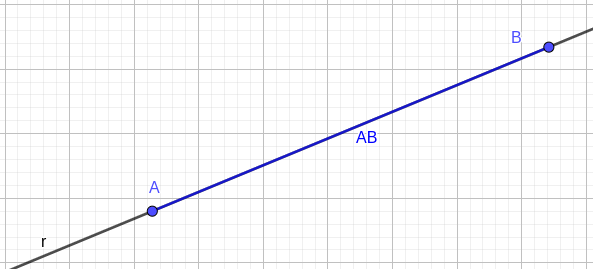
\includegraphics[width=0.6\textwidth]{./cap_vetor/dados/fig_segmento/fig_segmento}
  \caption{Esboço de um segmento $AB$.}
  \label{fig:segmento}
\end{figure}

\subsubsection{Norma e direção}

Associado a um segmento $AB$, temos sua \emph{norma}\index{norma} a qual é denotada por $|AB|$ e é definida como a distância entre seus pontos extremos $A$ e $B$. Ou seja, a norma do segmento $AB$ é a medida de seu comprimento ou tamanho.

A {\bf direção}\index{direção} de um segmento $AB$ é a direção de sua reta suporte, i.e. a direção da reta que fica determinada pelos pontos $A$ e $B$. Logo, dois segmentos $AB$ e $CD$ têm a mesma direção, quando suas retas suportes são paralelas ou coincidentes (ou seja, elas têm a mesma direção).

\begin{ex}\label{ex:segmento}
  Consideremos os segmentos esboçados na Figura \ref{fig:ex_segmento}. Os segmentos $AB$ e $CD$ têm as mesmas direções, mas comprimentos diferentes. Já, o segmento $EF$ tem direção diferente dos segmentos $AB$ e $CD$.
  
  \begin{figure}[H]
    \centering
    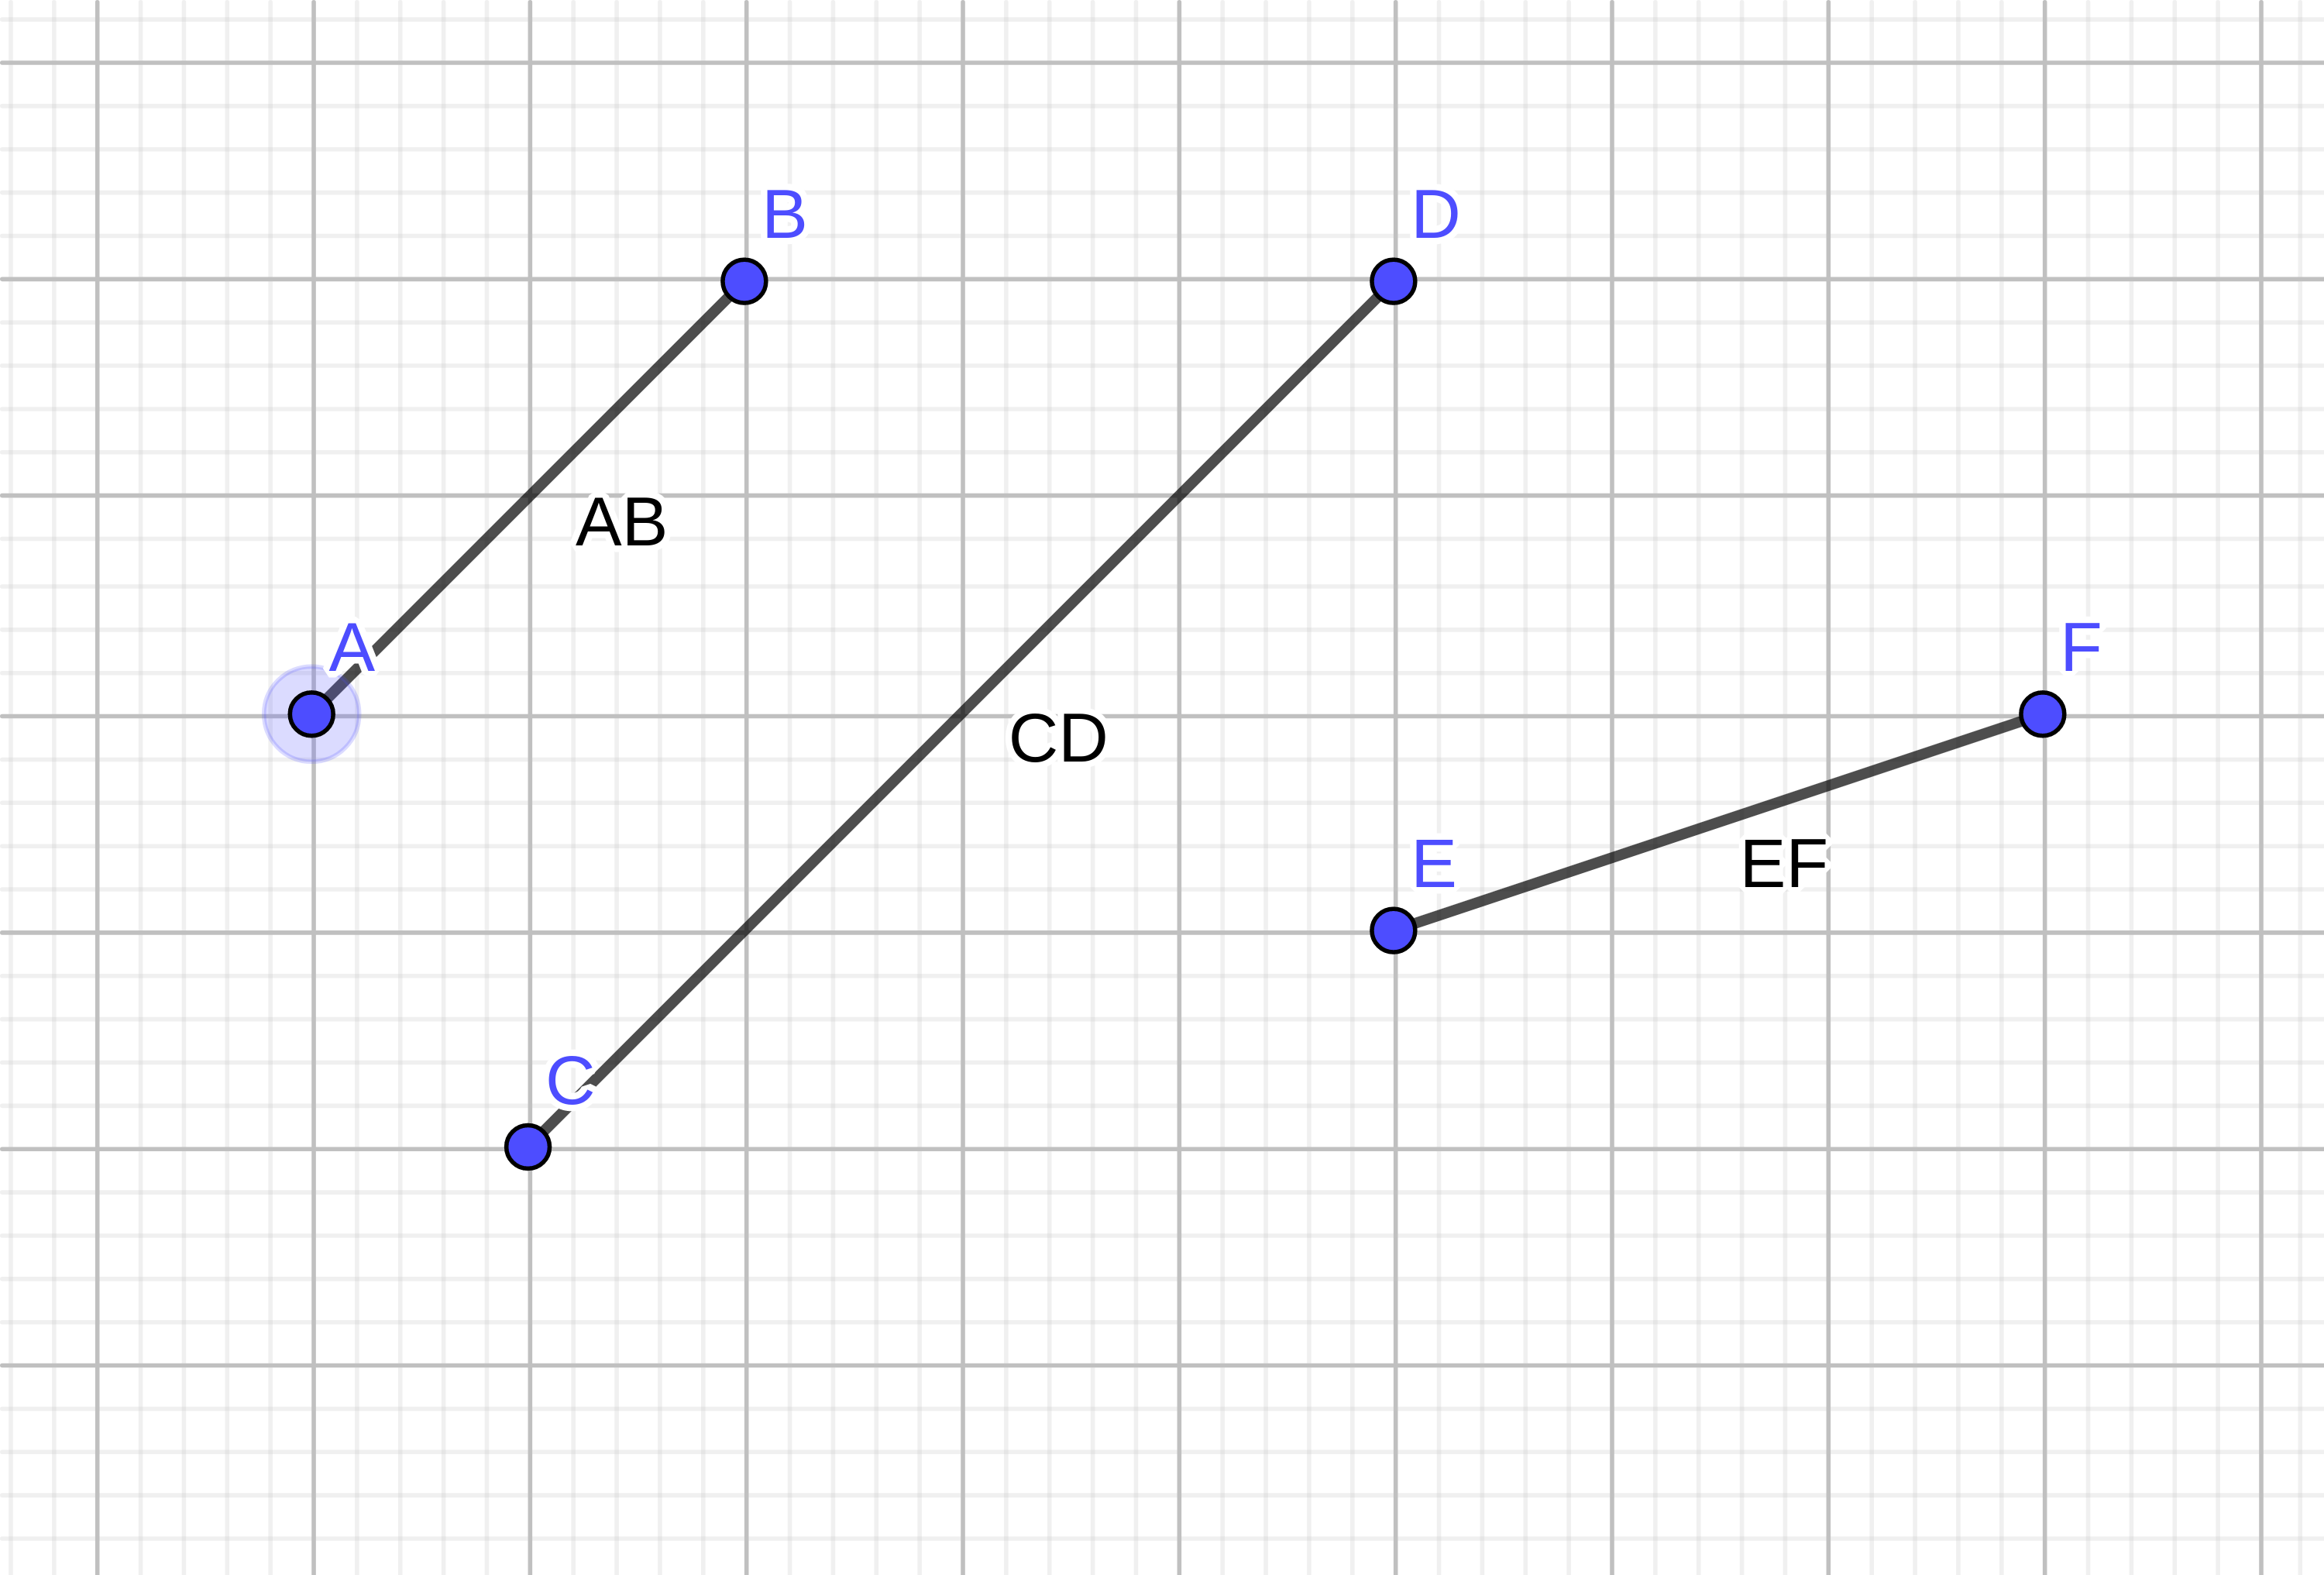
\includegraphics[width=0.6\textwidth]{./cap_vetor/dados/fig_ex_segmento/fig_ex_segmento}
  \caption{Esboço referente ao Exemplo \ref{ex:segmento}.}
  \label{fig:ex_segmento}
\end{figure}
\end{ex}

\subsubsection{Segmento nulo}

Se $A$ e $B$ são pontos coincidentes, então chamamos $AB$ de {\bf segmento nulo}\index{segmento nulo} e temos $|AB| = 0$. Observamos que a representação geométrica de um segmento nulo é um ponto, tendo em vista que seus pontos extremos são coincidentes. Como existem infinitas retas de diferentes direções que passam por um único ponto, temos que segmentos nulos não têm direção definida.

\subsection{Segmento orientado}

\begin{flushright}
  \href{https://archive.org/details/definicao-segmento-orientado}{$\blacktriangleright$ Vídeo disponível!}
\end{flushright}

Observamos que um dado segmento $AB$ é igual ao segmento $BA$. Agora, podemos associar a noção de {\bf sentido} a um segmento, escolhendo um dos pontos como sua {\bf origem}\index{origem} (ou \emph{ponto de partida}) e o outro como sua {\bf extremidade}\index{extremidade} (ou \emph{ponto de chegada}). Ao fazermos isso, definimos um {\bf segmento orientado}\index{segmento orientado}.

Mais precisamente, um segmento orientado $AB$ é o segmento definido pelos pontos $A$ e $B$, sendo $A$ o ponto de partida (origem) e $B$ o ponto de chegada (extremidade). Veja a Figura \ref{fig:seg_orientado}.

\begin{figure}[H]
  \centering
  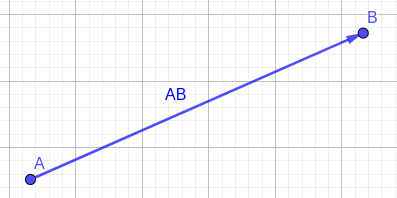
\includegraphics[width=0.5\textwidth]{./cap_vetor/dados/fig_seg_orientado/fig_seg_orientado}
  \caption{Esboço de um segmento orientado $AB$.}
  \label{fig:seg_orientado}
\end{figure}

\subsubsection{Norma e direção}

As noções de norma e de direção para segmentos estendem-se diretamente a segmentos orientados. Dizemos que dois dados segmentos orientados não nulos $AB$ e $CD$ têm a {\bf mesma direção} quando as retas $AB$ e $CD$ são paralelas ou coincidentes. A norma de um segmento orientado $AB$ é a norma do segmento $AB$, denotada por $|AB|$. O segmento orientado nulo $AA$ tem norma $|AA|=0$ e não tem direção definida.

\begin{ex}\label{ex:segorien_direcao}
  Consideremos os segmentos orientados esboçados na Figura \ref{fig:ex_segorien_direcao}. Observemos que os segmentos orientados $AB$ e $CD$ têm a mesma direção. Já o segmento orientado $EF$ tem direção diferente dos segmentos $AB$ e $CD$.
  
  \begin{figure}[H]
    \centering
    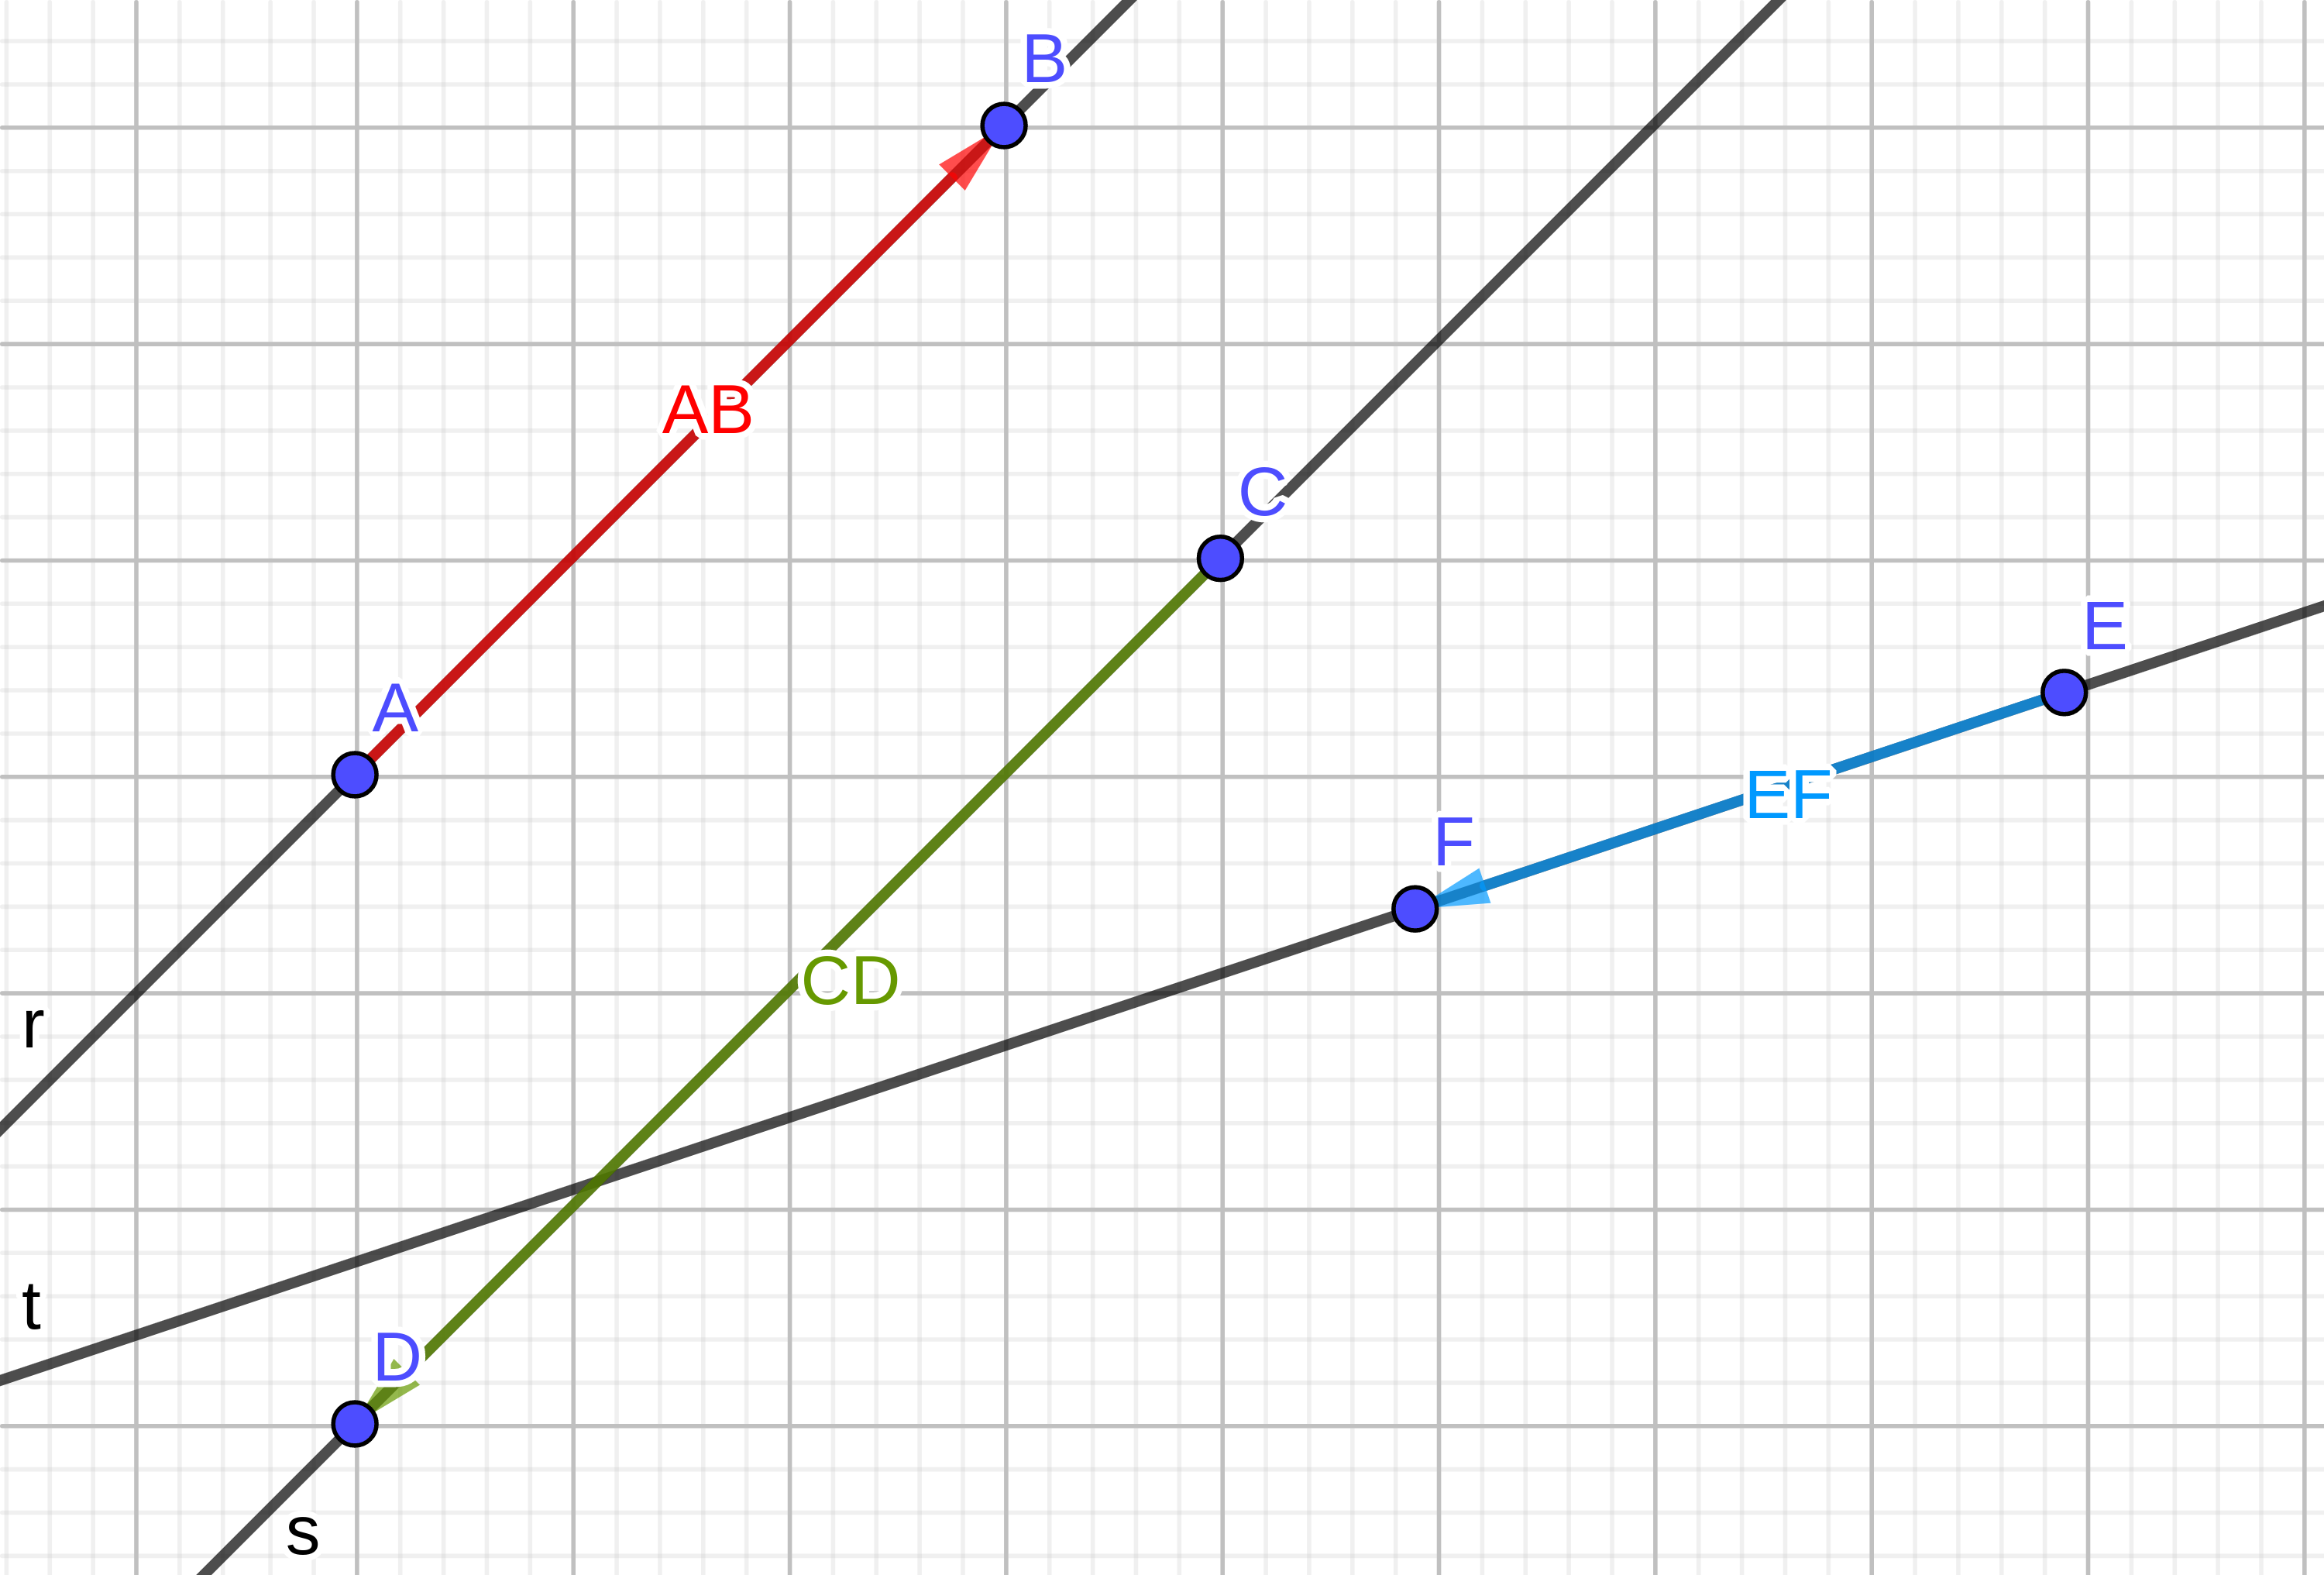
\includegraphics[width=0.7\textwidth]{./cap_vetor/dados/fig_ex_segorien_direcao/fig_ex_segorien_direcao}
  \caption{Esboço referente ao Exemplo \ref{ex:segorien_direcao}.}
  \label{fig:ex_segorien_direcao}
\end{figure}  
\end{ex}

\subsubsection{Comparação do sentido}

\begin{flushright}
  \href{https://archive.org/details/comparacao-sentido-segmentos-orientados}{$\blacktriangleright$ Vídeo disponível!}
\end{flushright}

Segmentos orientados $AB$ e $CD$ de mesma direção podem ter o mesmo sentido ou sentidos opostos. No caso de suas retas suportes não serem coincidentes, os segmentos orientados $AB$ e $CD$ têm a mesma direção, quando os segmentos $AC$ e $BD$ não se interceptam. E, caso estas se intercetam, os segmentos orientados $AB$ e $CD$ têm sentidos opostos. 

\begin{ex}
  Na Figura \ref{fig:segorien_sentido}, temos que os segmentos $AB$ e $CD$ têm o mesmo sentido. De fato, observamos que eles têm a mesma direção e que os segmentos $AC$ e $BD$ têm interseção vazia.

\begin{figure}[H]
  \centering
  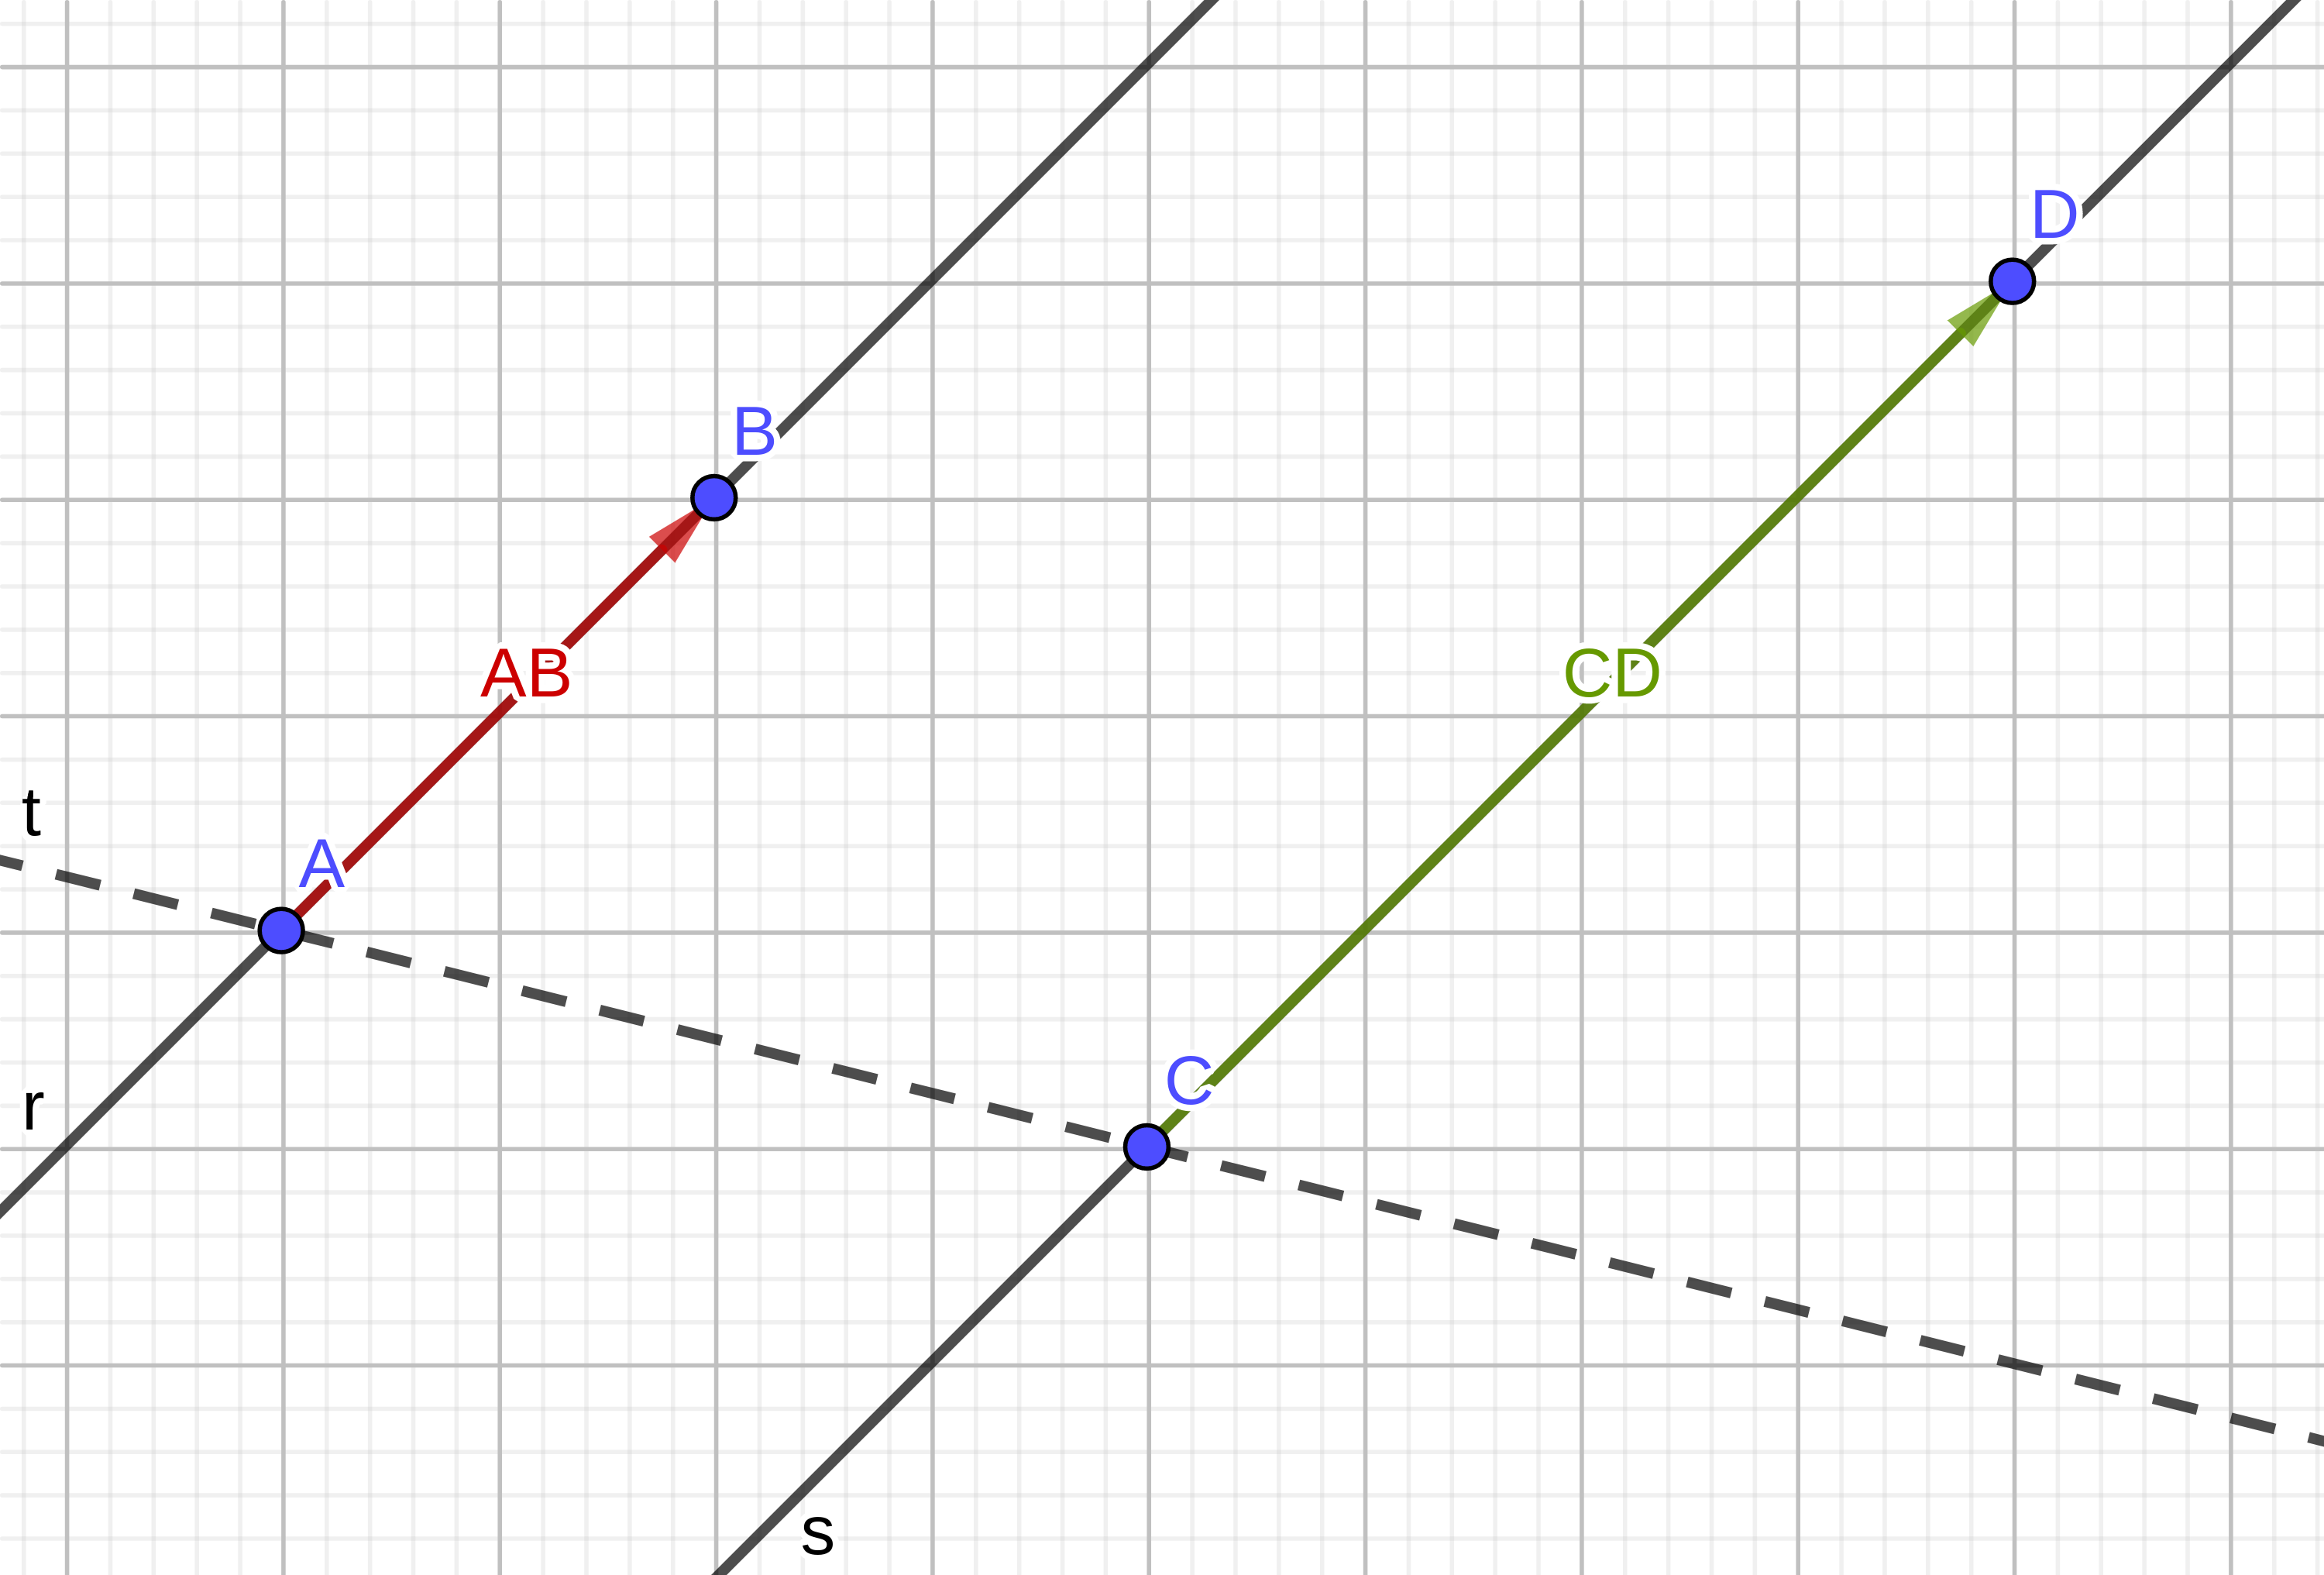
\includegraphics[width=0.7\textwidth]{./cap_vetor/dados/fig_segorien_sentido/fig_segorien_sentido}
  \caption{Segmentos orientados $AB$ e $CD$ de mesmo sentido. Segmentos orientados $EF$ e $GH$ de sentidos opostos.}
  \label{fig:segorien_sentido}
\end{figure}

Na mesma Figura \ref{fig:segorien_sentido}, vemos que os segmentos orientados $EF$ e $GH$ têm sentidos opostos, pois têm a mesma direção e os segmentos $EG$ e $FH$ se interceptam (no ponto $I$). 
\end{ex}

\begin{obs}\label{obs:segorin_sentido_trans}
  A propriedade de segmentos orientados terem o mesmo sentido é transitiva. Ou seja, se $AB$ e $CD$ têm o mesmo sentido e $CD$ e $EF$ têm o mesmo sentido, então $AB$ e $EF$ têm o mesmo sentido.
\end{obs}

Com base na Observação \ref{obs:segorin_sentido_trans}, analisamos o sentido de dois segmentos orientados e colineares escolhendo um deles e construíndo um segmento orientado de mesmo sentido  e não colinear. Então, analisamos o sentido dos segmentos orientados originais com respeito ao introduzido.

\subsubsection{Equipolência}

\begin{flushright}
  \href{https://archive.org/details/segmentos-orientados-equipolentes}{$\blacktriangleright$ Vídeo disponível!}
\end{flushright}

Um segmento orientado não nulo $AB$ é \emph{equipolente}\index{segmento orientado!equipolente} a um segmento orientado $CD$, quando $AB$ tem a \emph{mesma norma}, a \emph{mesma direção} e o \emph{mesmo sentido} de $CD$. Segmentos nulos também são considerados equipolentes entre si. Quando $AB$ é equipolente a $CD$, escrevemos $AB \sim CD$.

\begin{figure}[H]
  \centering
  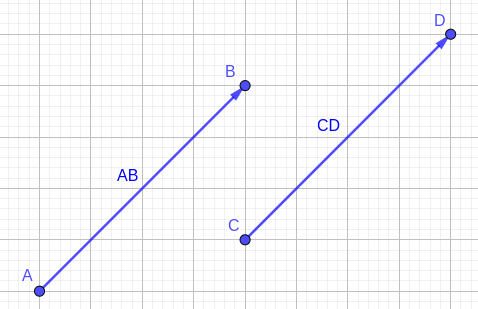
\includegraphics[width=0.7\textwidth]{./cap_vetor/dados/fig_segequipolentes/fig_segequipolentes}
  \caption{Esboço de dois segmentos orientados $AB$ e $CD$ equipolentes.}
  \label{fig:segequipolentes}
\end{figure}

A relação de equipolência é uma \emph{relação de equivalência}. De fato, temos:
\begin{itemize}
\item \emph{relação reflexiva}: $AB \sim AB$;
\item \emph{relação simétrica}: $AB \sim CD \Rightarrow CD \sim AB$;
\item \emph{relação transitiva}: $AB \sim CD ~ \text{e} ~ CD \sim EF \Rightarrow AB \sim CD$.
\end{itemize}

Com isso, dado um segmento $AB$, definimos a \emph{classe de equipolência} de $AB$ como o conjunto de todos os segmentos equipolentes a $AB$. O segmento $AB$ é um \emph{representante} desta classe.

\subsection*{Exercícios resolvidos}

\begin{exeresol}
  Mostre que dois segmentos orientados $AB$ e $CD$ são equipolentes se, e somente se, os pontos médios de $AD$ e $BC$ são coincidentes.
\end{exeresol}
\begin{resol}
  Começamos mostrando a implicação. Por hipótese, temos que $AB$ e $CD$ são equipolentes. A tese é clara no caso de $AB$ e $CD$ serem coincidentes. Vejamos, então, o caso em que $AB$ e $CD$ não são coincidentes. Desta forma, $ABCD$ determina um paralelogramo de diagonais $AD$ e $BC$. Como as diagonais de um paralelogramo se interceptam em seus pontos médios, temos demonstrado a implicação.

  Agora, mostramos a recíproca. Por hipótese, temos que os pontos médios de $AD$ e $BC$ são coincidentes. Novamente, se $AD$ e $BD$ são coincidentes a conclusão é direta. Consideremos o caso em que $AD$ e $BD$ não são coincidentes. Daí, segue que $AB$ e $CD$ têm o mesmo tamanho e mesma direção. Seja $M$ o ponto médio de $AD$ e $BC$ e $\pi$ o plano determinado pelos segmentos $AB$ e $CD$. Notando que $M$, $B$ e $D$ estão no mesmo semiplano de $\pi$ determinado pela reta $AC$, concluímos que $AB$ e $CD$ são equipolentes.
\end{resol}

\begin{exeresol}
  Mostre que $AB\sim CD$, então $BA\sim DC$.
\end{exeresol}
\begin{resol}
  $AB$ e $BA$ têm o mesmo tamanho e direção. $CD$ e $DC$ têm o mesmo tamanho e direção. Como $AB\sim CD$, temos que $BA$ e $DC$ têm o mesmo tamanho e direção. Por fim, observa-se que $BA$ e $DC$ têm ambos o mesmo sentido oposto de $AB$ e $DC$. 
\end{resol}

\subsection*{Exercícios}

\begin{exer}
  Faça o esboço de dois segmentos $AB$ e $CD$ com $|AB|\neq |CD|$ e cujas retas determinadas por eles sejam coincidentes.
\end{exer}

\begin{exer}
  Faça o esboço de dois segmentos orientados $AB\not\sim CD$ e de mesmo sentido.
\end{exer}

\begin{exer}
  Faça o esboço de dois segmentos orientados colineares, de tamanhos iguais e sentidos opostos.
\end{exer}

\begin{exer}
  Diga se é verdadeira ou falsa a seguinte afirmação: é quadrado todo trapézio retângulo $ABCD$ com segmentos orientados $AD$ e $BC$ equipolentes. Justifique sua afirmação. 
\end{exer}
\begin{resp}
  Verdadeira.
\end{resp}

\begin{exer}
  Mostre que $AB\sim CD$, então $AC\sim BD$.
\end{exer}
\begin{resp}
  Dica: $ABCD$ determina um paralelogramo.
\end{resp}

\begin{exer}
  Mostre que se $AC\sim CB$, então $C$ é ponto médio do segmento $AB$.
\end{exer}

\section{Vetor}\label{cap_vetor_sec_vetor}

\begin{flushright}
  \href{https://archive.org/details/definicao-vetor}{$\blacktriangleright$ Vídeo disponível!}
\end{flushright}

Dado um segmento orientado $AB$, define-se o vetor $\overrightarrow{AB}$ (lê-se vetor $AB$), a classe de equipolência de $AB$. Um segmento orientado da classe é um representante (geométrica) do vetor. A Figura \ref{fig:vetor} mostra duas representações de um dado vetor $\vec{u} = \overrightarrow{AB}$.

\begin{figure}[H]
  \centering
  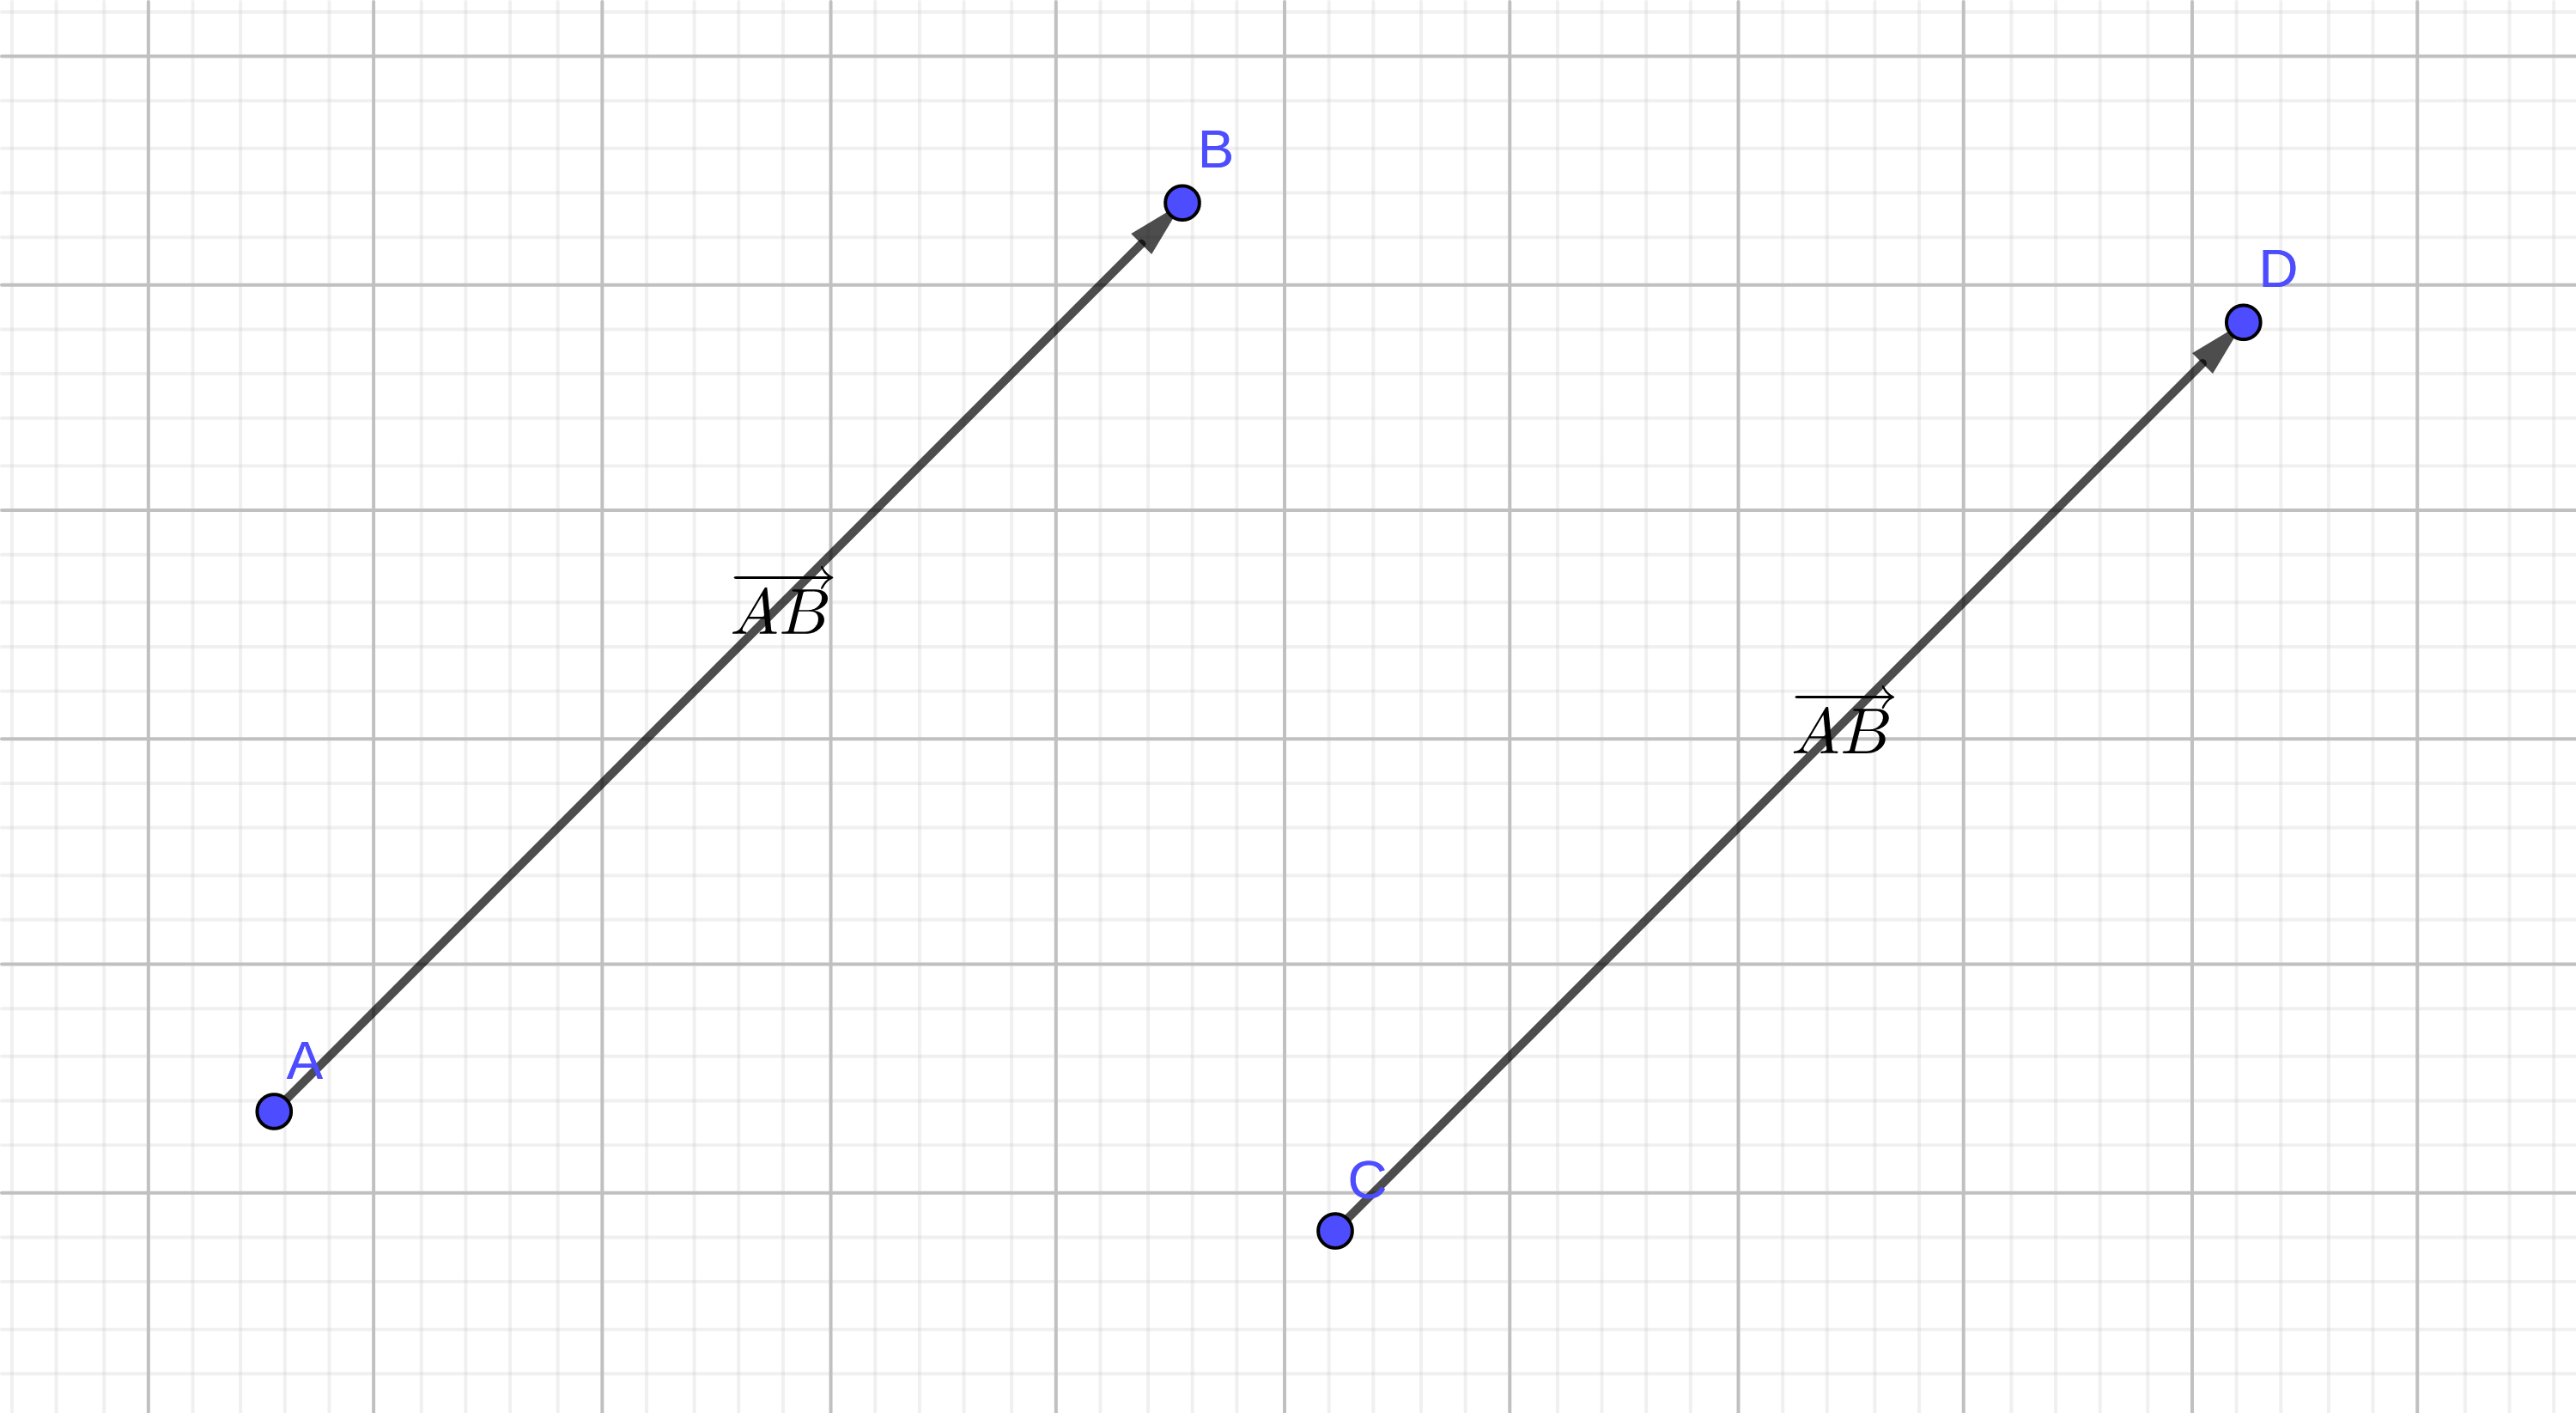
\includegraphics[width=0.7\textwidth]{./cap_vetor/dados/fig_vetor/fig_vetor}
  \caption{Esboço de duas representações de dado vetor $\vec{u}$.}
  \label{fig:vetor}
\end{figure}

O \emph{vetor nulo} é aquele que tem como representante um segmento orientado nulo. É denotado por $\vec{0}$ e geometricamente representado por um ponto.

A \emph{norma} (ou módulo) de um vetor $\vec{u}$ é denotada(o) por $|\vec{u}|$ e é definido como a norma de qualquer uma de suas representações. Mais precisamente, se o segmento orientado $AB$ é uma representação de $\vec{v}$, i.e. $\vec{v} = \overrightarrow{AB}$, então
\begin{equation}
|\vec{v}| = |\overrightarrow{AB}| := |AB|
\end{equation}

\begin{obs}
  $|\vec{v}| = 0$ se, e somente se, $\vec{v} = \vec{0}$.

  Seja $\vec{v} = \overrightarrow{AB}$. Lembrando que $|\overrightarrow{AB}| = |AB|$, i.e. a distância entre os pontos $A$ e $B$, segue que se $\vec{v} = \vec{0}$, então $AB$ é um segmento orientado nulo e, portanto, $0=|AB|=|\vec{v}|$. Reciprocamente, se $|\vec{v}| = 0$, então $|AB| = 0$ e, portanto, $AB$ é um segmento orientado nulo, i.e. $A$ e $B$ são pontos sobrepostos (coincidentes) e $\overrightarrow{AB} = \vec{0}$.
\end{obs}

Dois {\bf vetores} são ditos {\bf paralelos} \index{vetores!paralelos} quando qualquer de suas representações têm a mesma direção. De forma análoga, definem-se {\bf vetores coplanares}\index{vetores!coplanares}, {\bf vetores não coplanares}\index{vetores!não coplanares}, {\bf vetores ortogonais}\index{vetores!ortogonais}, além de conceitos como {\bf ângulo entre dois vetores}\index{ângulo!entre vetores}, etc.


\begin{ex}
  Vejamos a Figura \ref{fig:vetorrel}. Temos os vetores paralelos $\vec{u}$ e $\vec{v}$, equanto que os vetores $\vec{s}$ e $\vec{t}$ são ortogonais (ou perpendiculares).

  \begin{figure}[H]
  \centering
  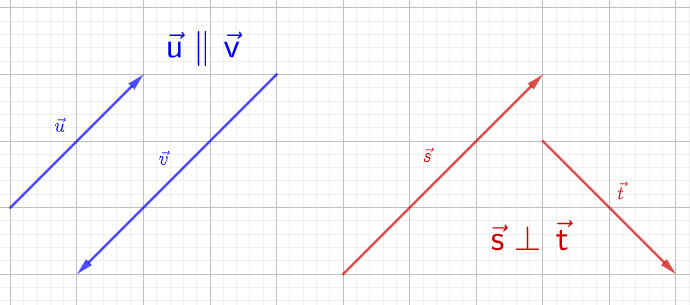
\includegraphics[width=0.7\textwidth]{./cap_vetor/dados/fig_vetorrel/fig_vetorrel}\\
  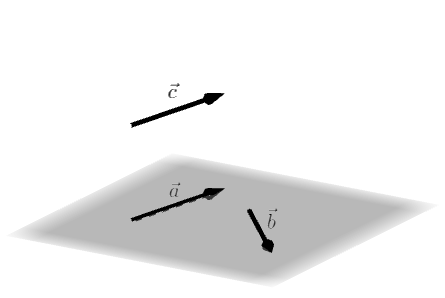
\includegraphics[width=0.5\textwidth]{./cap_vetor/dados/fig_vcolineares/fig_vcolineares}
  \caption{Esquerda: esboços de vetores paralelos e de vetores ortogonais. Direita: esboços de vetores coplanares.}
  \label{fig:vetorrel}
\end{figure}

Também da Figura \ref{fig:vetorrel}, temos que os vetores $\vec{a}$, $\vec{b}$ e $\vec{c}$ são coplanares. Embora, na figura $\vec{c}$ está representado fora do plano determinado pelas representações de $\vec{a}$ e $\vec{b}$, podemos tomar uma outra representação de $\vec{c}$ coplanar a estas representações.
\end{ex}


\subsection{Adição de vetores}

\begin{flushright}
  \href{https://archive.org/details/adicao-de-vetores}{$\blacktriangleright$ Vídeo disponível!}
\end{flushright}

Sejam dados dois vetores $\vec{u}$ e $\vec{v}$. Sejam, ainda, uma representação $\overrightarrow{AB}$ de $\vec{u}$ e uma representação $\overrightarrow{BC}$ do vetor $\vec{v}$. Então, define-se o vetor soma $\vec{u}+\vec{v}$ como o vetor representado por $\overrightarrow{AC}$. Veja a Figura \ref{fig:vadicao}.

\begin{figure}[H]
  \centering
  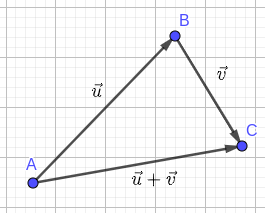
\includegraphics[width=0.5\textwidth]{./cap_vetor/dados/fig_vadicao/fig_vadicao}
  \caption{Representação geométrica da adição de dois vetores.}
  \label{fig:vadicao}
\end{figure}

\begin{obs}
  Vejamos as seguintes propriedades:
  \begin{enumerate}[a)]
  \item Elemento neutro na adição:
    \begin{equation}
      \vec{u} + \vec{0} = \vec{u}
    \end{equation}
    
    De fato, seja $\vec{u} = \overrightarrow{AB}$. Observamos que podemos representar $\vec{0} = \overrightarrow{BB}$. Logo, temos $\vec{u} + \vec{0} = \overrightarrow{AB} + \overrightarrow{BB} = \overrightarrow{AB} = \vec{u}$.

  \item Associatividade na adição:
    \begin{equation}
      (\vec{u} + \vec{v}) + \vec{w} = \vec{u} + (\vec{v} + \vec{w}).
    \end{equation}

    De fato, sejam $\vec{u} = \overrightarrow{AB}$, $\vec{v} = \overrightarrow{BC}$ e $\vec{w} = \overrightarrow{CD}$. Então, segue
    \begin{align}
      \left(\vec{u} + \vec{v}\right)+\vec{w} &= \left(\overrightarrow{AB}+\overrightarrow{BC}\right)+\overrightarrow{CD} \\
                                             &= \overrightarrow{AC} + \overrightarrow{CD} \\
                                             &= \overrightarrow{AD},
    \end{align}
    bem como,
    \begin{align}
      \vec{u} + \left(\vec{v} + \vec{w}\right) &= \overrightarrow{AB}+\left(\overrightarrow{BC}+\overrightarrow{CD}\right) \\
                                             &= \overrightarrow{AB} + \overrightarrow{BD} \\
                                             &= \overrightarrow{AD}.
    \end{align}
  \item Comutatividade da adição:
    \begin{equation}
      \vec{u} + \vec{v} = \vec{v} + \vec{u}.
    \end{equation}

    Esta propriedade pode ser demonstrada usando a regra do paralelogramo que veremos mais adiante. Veja, também, o Exercício Resolvido \ref{exeresol:vetor_comuta_adicao}.
  \end{enumerate}
\end{obs}

\subsection{Vetor oposto}

\begin{flushright}
  \href{https://archive.org/details/vetor-oposto}{$\blacktriangleright$ Vídeo disponível!}
\end{flushright}

Um \pmb{vetor} $\vec{v}$ é dito ser \pmb{oposto} \index{vetor!oposto} a um dado vetor $\vec{u}$, quando quaisquer representações de $\vec{u}$ e $\vec{v}$ são segmentos orientados de mesmo comprimento e mesma direção, mas com sentidos opostos. Neste caso, denota-se por $-\vec{u}$ o vetor oposto a $\vec{u}$. Veja a Figura \ref{fig:voposto}.

\begin{figure}[H]
  \centering
  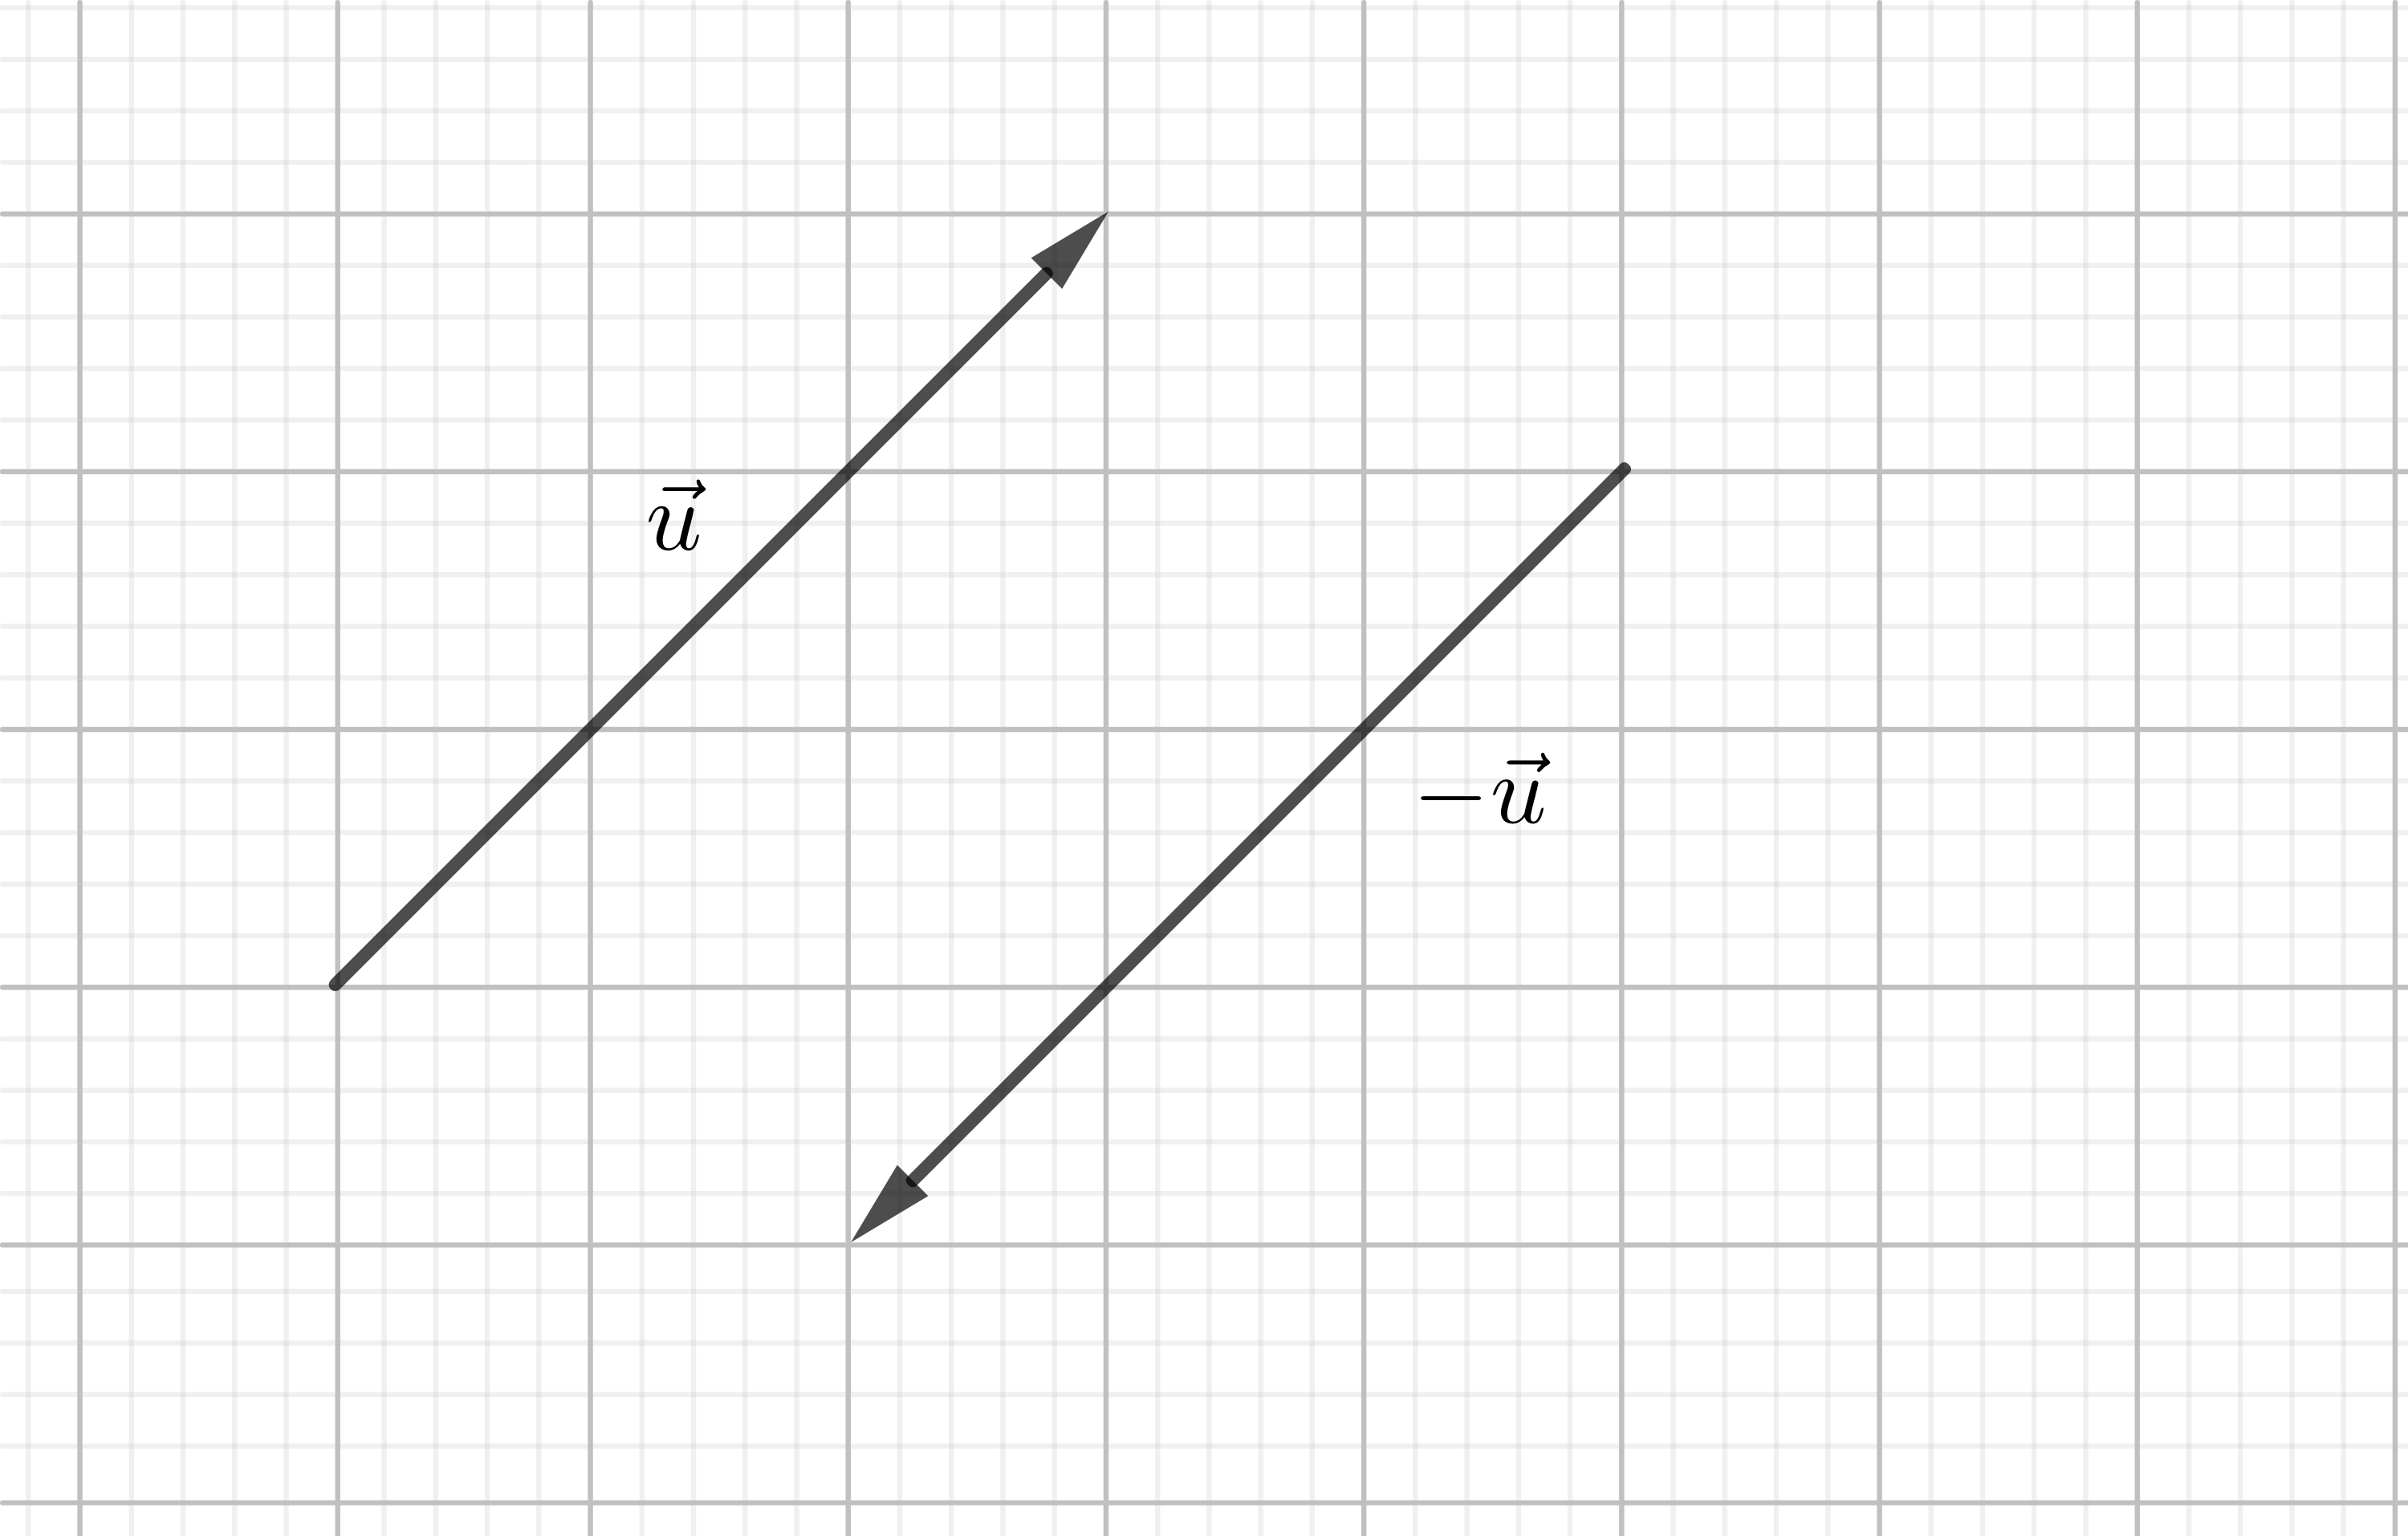
\includegraphics[width=0.5\textwidth]{./cap_vetor/dados/fig_voposto/fig_voposto}
  \caption{Representação geométrica de vetores opostos.}
  \label{fig:voposto}
\end{figure}

\begin{obs}
  $|\vec{v}| = |-\vec{v}|$.

  De fato, seja $\vec{v} = \overrightarrow{AB}$. Então, $|\vec{v}| = |AB| = |BA| = |-\vec{v}|$.
\end{obs}

\begin{obs}(Existência do oposto)
  \begin{equation}
    \vec{u} + \left(-\vec{u}\right) = \vec{0}.
  \end{equation}

  De fato, seja $\vec{u} = \overrightarrow{AB}$. Então, $-\vec{u} = -\overrightarrow{AB} = \overrightarrow{BA}$. Segue que
  \begin{align}
    \vec{u} + \left(-\vec{u}\right) &= \overrightarrow{AB} + \left(-\overrightarrow{AB}\right) \\
                                    &= \overrightarrow{AB} + \overrightarrow{BA} \\
                                    &= \overrightarrow{AA} \\
                                    &= \vec{0}.
  \end{align}
\end{obs}

\subsection{Subtração de vetores}

\begin{flushright}
  \href{https://archive.org/details/subtracao-de-vetores}{$\blacktriangleright$ Vídeo disponível!}
\end{flushright}

Sejam dados dois vetores $\vec{u}$ e $\vec{v}$. A subtração de $\vec{u}$ com $\vec{v}$ é denotada por $\vec{u}-\vec{v}$ e é definida pela adição de $\vec{u}$ com $-\vec{v}$, i.e. $\vec{u}-\vec{v}=\vec{u}+(-\vec{v})$. Veja a Figura \ref{fig:vsubtracao}.

\begin{figure}[H]
  \centering
  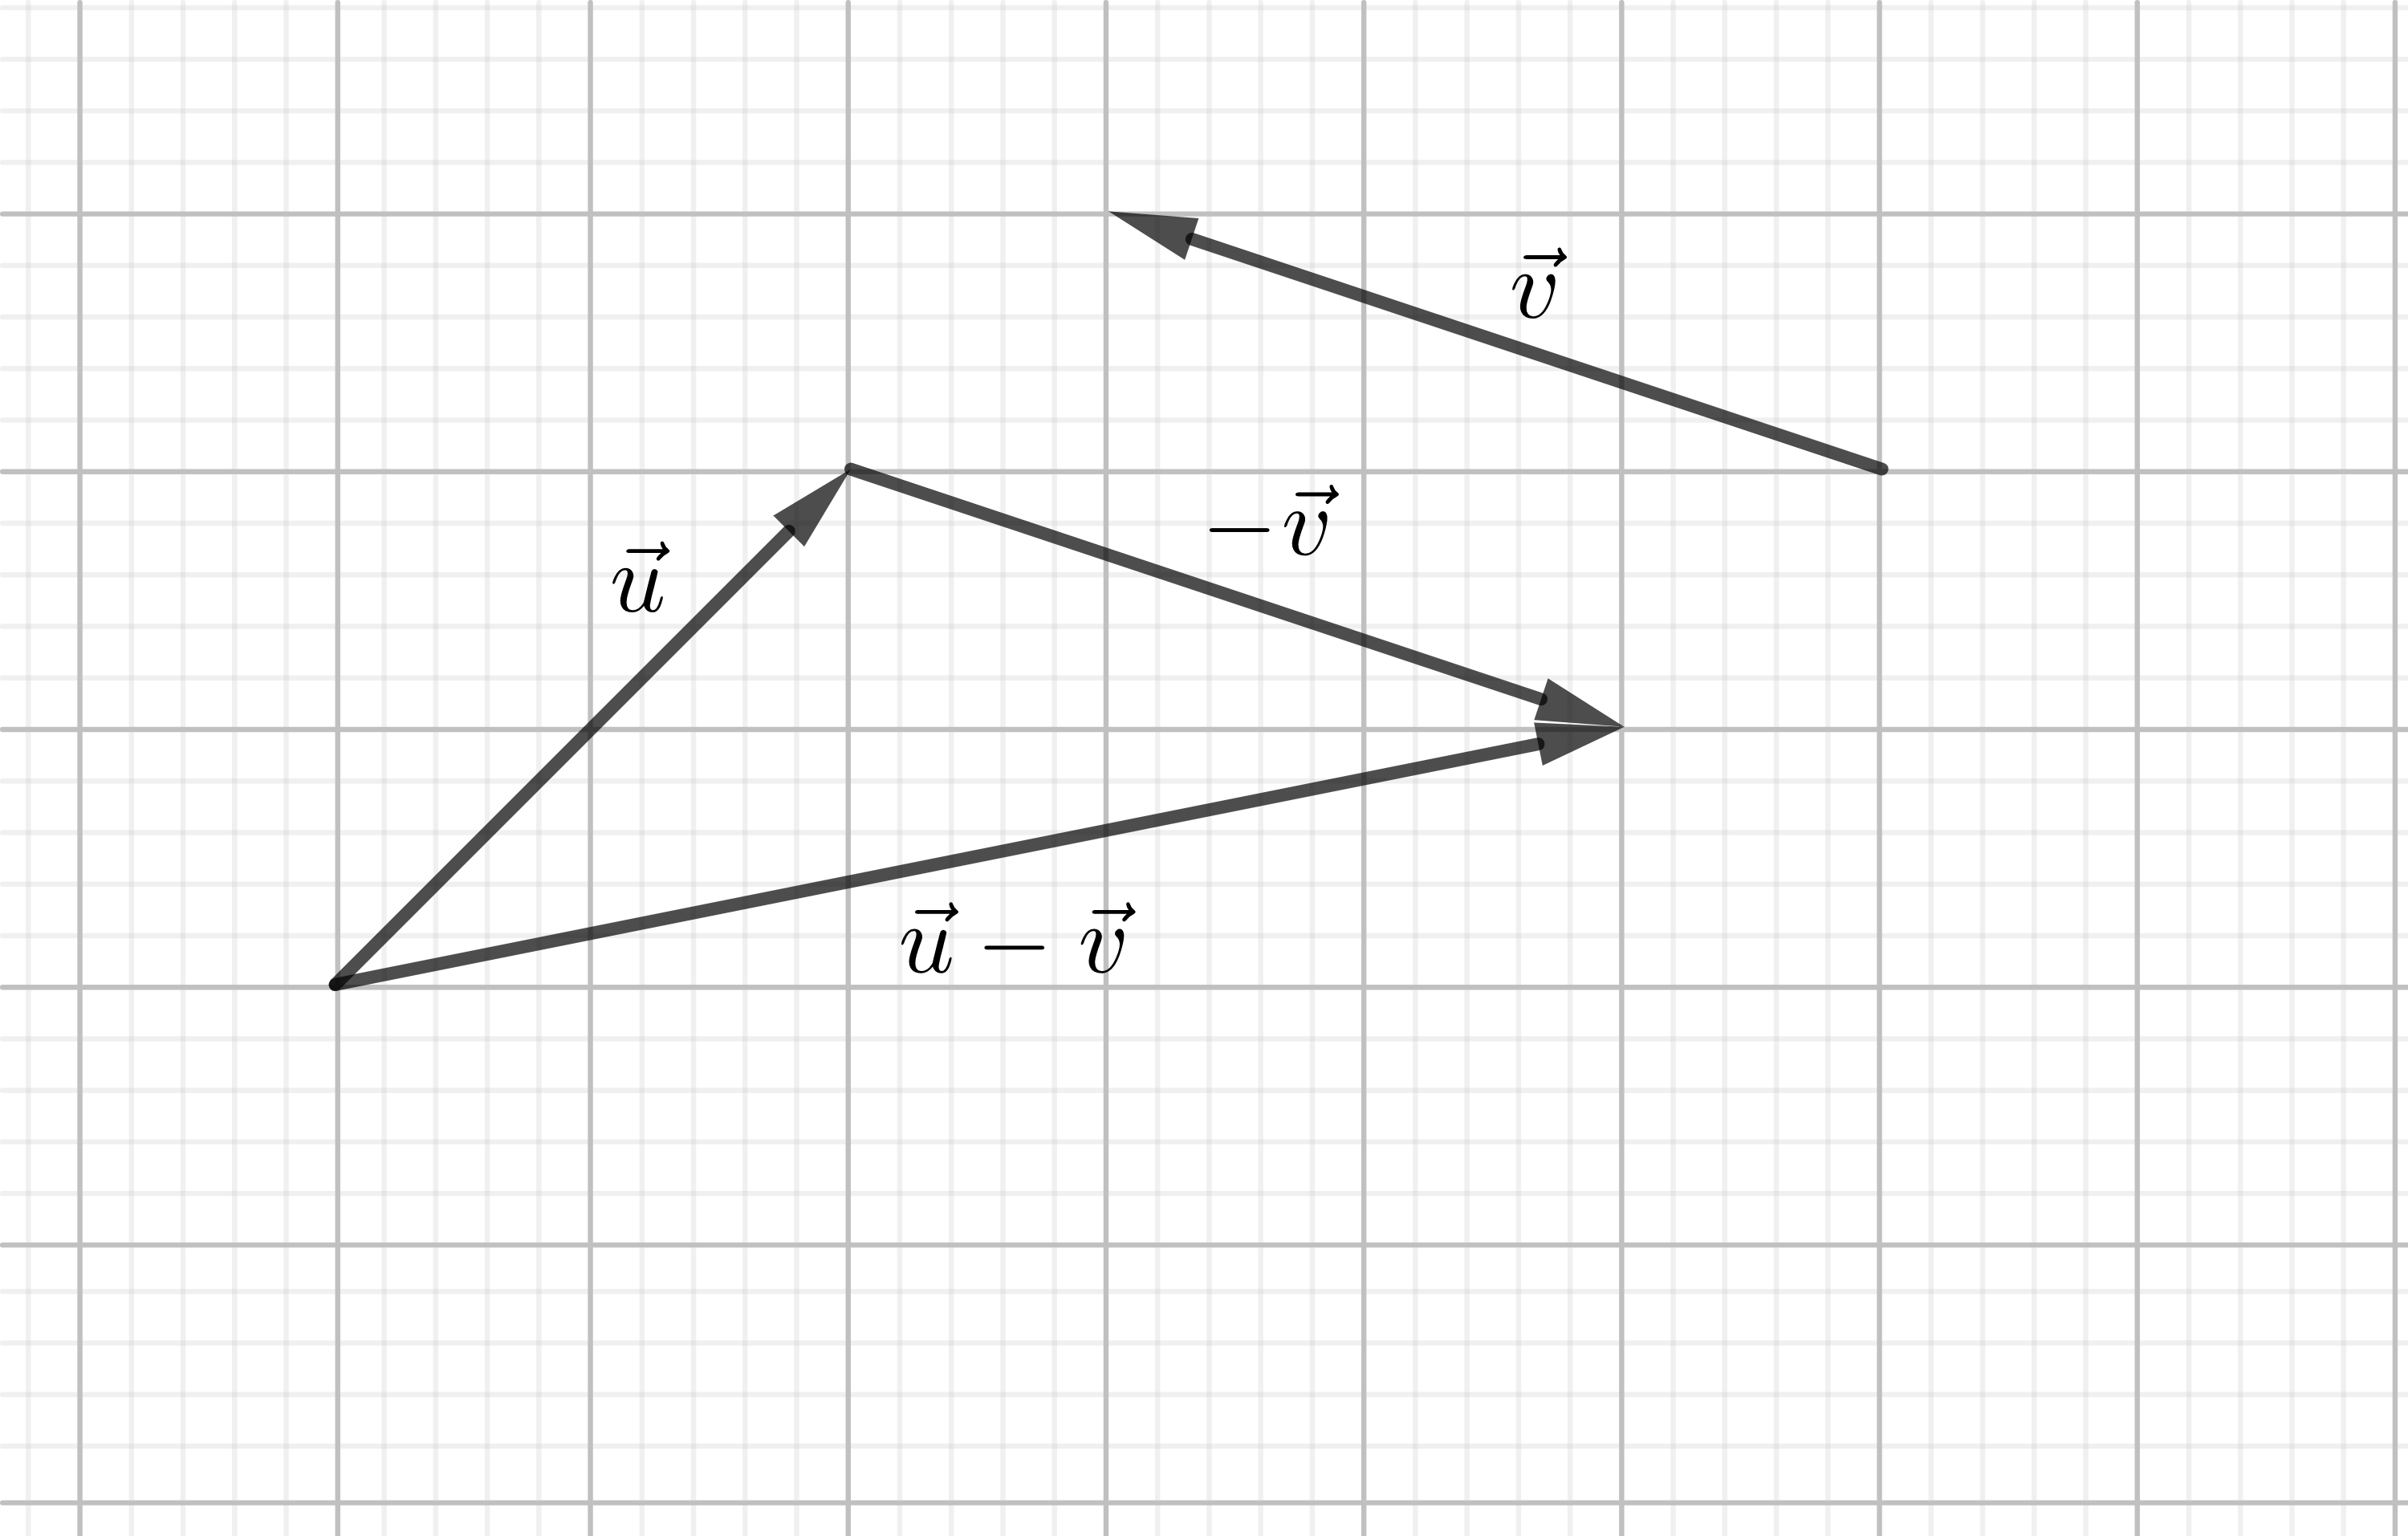
\includegraphics[width=0.5\textwidth]{./cap_vetor/dados/fig_vsubtracao/fig_vsubtracao}
  \caption{Representação geométrica da subtração de $\vec{u}$ com $\vec{v}$, i.e. $\vec{u}-\vec{v}$.}
  \label{fig:vsubtracao}
\end{figure}

\begin{obs}\normalfont{(Regra do paralelogramo)}
  \begin{flushright}
    \href{https://archive.org/details/regra-do-paralelogramo}{$\blacktriangleright$ Vídeo disponível!}
  \end{flushright}

  Sejam vetores não nulos $\vec{u} = \overrightarrow{AB}$ e $\vec{v} = \overrightarrow{AD}$. Seja, ainda, $C$ o vértice oposto ao $A$ no paralelogramo determinado pelos lados formados pelos segmentos $AB$ e $AD$. Então, temos $\vec{u} + \vec{v} = \overrightarrow{AC}$ e $\vec{u}-\vec{v} = \overrightarrow{DB}$. Veja a Figura \ref{fig:regrapara}.

\begin{figure}[H]
  \centering
  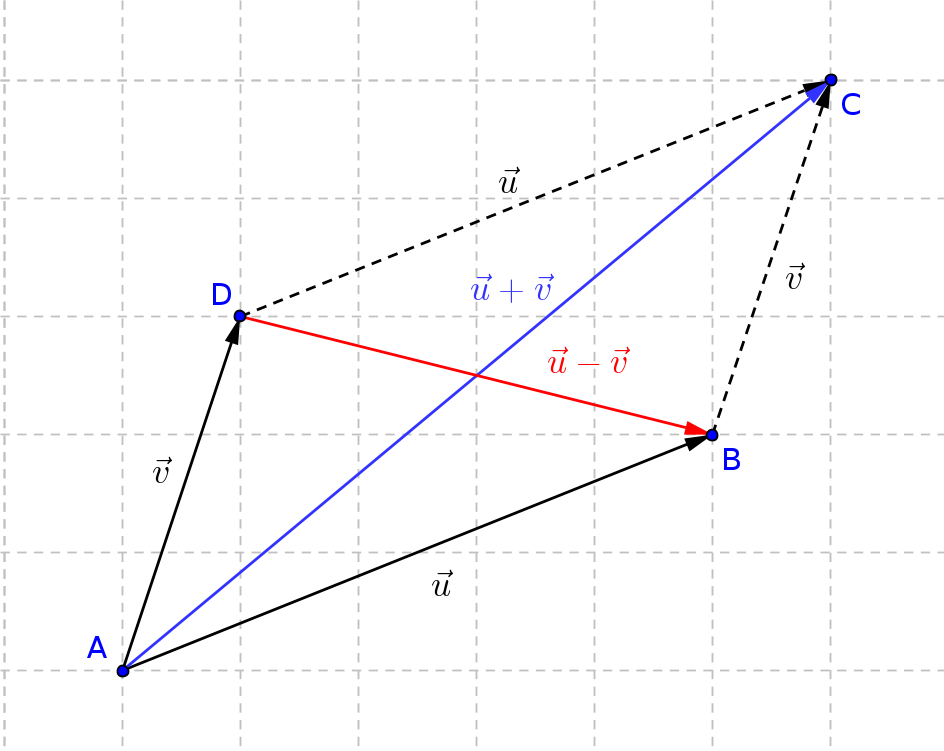
\includegraphics[width=0.6\textwidth]{./cap_vetor/dados/fig_regrapara/fig_regrapara}
  \caption{Regra do paralelogramo para a presentação geométrica da soma e da diferença de vetores.}
  \label{fig:regrapara}
\end{figure}  
\end{obs}

\subsection{Multiplicação de vetor por um escalar}

\begin{flushright}
  \href{https://archive.org/details/multiplicacao-vetor-por-escalar}{$\blacktriangleright$ Vídeo disponível!}
\end{flushright}

A multiplicação de um número real $\alpha>0$ (escalar) por um vetor $\vec{u}$ é denotado por $\alpha\vec{u}$ e é definido pelo vetor de mesma direção e mesmo sentido de $\vec{u}$ com norma $\alpha|\vec{u}|$. Quando $\alpha = 0$, define-se $\alpha\vec{u}=\vec{0}$, i.e. o vetor nulo (geometricamente, representado por qualquer ponto).

\begin{obs}
  Notamos que:
  \begin{itemize}
  \item Para $\alpha<0$, temos $\alpha\vec{u} = -(-\alpha\vec{u})$.
  \item $|\alpha\vec{u}|=|\alpha||\vec{u}|$.
\end{itemize}
\end{obs}

\begin{figure}[H]
  \centering
  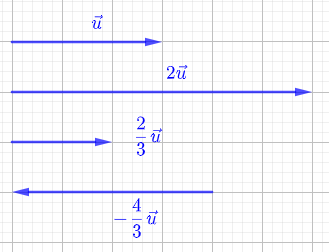
\includegraphics[width=0.6\textwidth]{./cap_vetor/dados/fig_vescalar/fig_vescalar}
  \caption{Representações geométricas de multiplicações de um vetor por diferentes escalares.}
  \label{fig:vescalar}
\end{figure}

\begin{obs}
  As seguintes propriedades são válidas:
  \begin{enumerate}[a)]
  \item Associatividade da multiplicação por escalar:
    \begin{equation}
      \alpha\left(\beta\vec{u}\right) = (\alpha\beta)\vec{u}
    \end{equation}

    De fato, em primeiro lugar, observamos que $\alpha\left(\beta\vec{u}\right)$ e $(\alpha\beta)\vec{u}$ têm a mesma direção e o mesmo sentido. Por fim, temos
    \begin{align}
      |\alpha\left(\beta\vec{u}\right)| &= |\alpha||\beta\vec{u}| \\
                                        &= |\alpha|\left(|\beta||\vec{u}|\right) \\
                                        &= \left(|\alpha||\beta|\right)|\vec{u}| \\
                                        &= |\alpha\beta||\vec{u}| \\
                                        &= |(\alpha\beta)\vec{u}|.
    \end{align}
    
  \item Distributividade:
    \begin{align}
      &(\alpha + \beta)\vec{u} = \alpha\vec{u} + \beta\vec{u}\\
      &\alpha\left(\vec{u}+\vec{v}\right) = \alpha\vec{u} + \alpha\vec{v}
    \end{align}
  \end{enumerate}
\end{obs}

\subsection{Resumo das propriedades das operações com vetores}

As operações de adição e multiplicação por escalar de vetores têm propriedades importantes. Para quaisquer vetores $\vec{u}$, $\vec{v}$ e $\vec{w}$ e quaisquer escalares $\alpha$ e $\beta$ temos:
\begin{itemize}
\item comutatividade da adição: $\vec{u}+\vec{v}=\vec{v}+\vec{u}$;
\item associatividade da adição: $(\vec{u} + \vec{v}) + \vec{w} = \vec{u} + (\vec{v} + \vec{w})$;
\item elemento neutro da adição: $\vec{u}+\vec{0}=\vec{u}$;
\item existência do oposto: $\vec{u}+(-\vec{u}) = \vec{0}$;
\item associatividade da multiplicação por escalar: $\alpha(\beta\vec{u})=(\alpha\beta)\vec{u}$;
\item distributividade da multiplicação por escalar:
  \begin{align}
    &\alpha(\vec{u}+\vec{v}) = \alpha\vec{u}+\alpha\vec{v},\\
    &(\alpha+\beta)\vec{u} = \alpha\vec{u}+\beta\vec{u};
  \end{align}
\item existência do elemento neutro da multiplicação por escalar: $1\vec{u}=\vec{u}$.
\end{itemize}

\subsection*{Exercícios resolvidos}

\begin{exeresol}
  Com base na figura abaixo, forneça o vetor $\overrightarrow{HC}$ como resultado de operações básicas envolvendo os vetores $\vec{u}$ e $\vec{v}$.
  \begin{figure}[H]
    \centering
    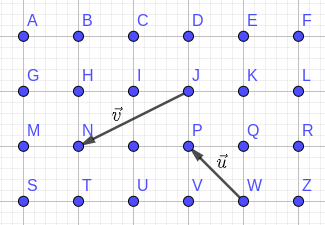
\includegraphics[width=0.7\textwidth]{./cap_vetor/dados/fig_exer_op_basicas/fig_vec_soma}
  \end{figure}
\end{exeresol}
\begin{resol}
  Vamos construir dois vetores auxiliares $\overrightarrow{HB}$ e $\overrightarrow{HI}$ a partir de operações envolvendo os vetores $\vec{u}$ e $\vec{v}$. Notamos que $\overrightarrow{HC} = \overrightarrow{HI} + \overrightarrow{HB}$.

  Começamos buscando formar o vetor $\overrightarrow{HI}$. Para tanto, observamos que $\vec{u}=\overrightarrow{NG}$ e, portanto, $\vec{v}+\vec{u}=\overrightarrow{JG}$. Com isso, obtemos que
  \begin{align}
    \overrightarrow{HI} &= -\frac{1}{3}\overrightarrow{JG} \\
                        &= -\frac{1}{3}(\vec{v}+\vec{u}).
  \end{align}

  Agora, vamos formar o vetor $\overrightarrow{HB}$. Isso pode ser feito da seguinte forma
  \begin{align}
    \overrightarrow{HB} &= \overrightarrow{WQ} \\
                        &= \vec{u} + \overrightarrow{PQ} \\
                        &= \vec{u} + \overrightarrow{HI} \\
                        &= \vec{u} -\frac{1}{3}(\vec{v}+\vec{u}) \\
                        &= \frac{2}{3}\vec{u} - \frac{1}{3}\vec{v}.
  \end{align}

  Por tudo isso, concluímos que
  \begin{align}
    \overrightarrow{HC} &= \overrightarrow{HI} + \overrightarrow{HB} \\
                        &= -\frac{1}{3}(\vec{v}+\vec{u}) \\
                        &+ \frac{2}{3}\vec{u} - \frac{1}{3}\vec{v} \\
                        &= \frac{1}{3}\vec{u} - \frac{2}{3}\vec{v}.
  \end{align}
\end{resol}

\begin{exeresol}\label{exeresol:vetor_comuta_adicao}
  Mostre que $\vec{u} + \vec{v} = \vec{v} + \vec{u}$.
\end{exeresol}
\begin{resol}
  Seja $ABCD$ o paralelogramo com $\vec{u} = \overrightarrow{AB} = \overrightarrow{DC}$ e $\vec{v} = \overrightarrow{AD} = \overrightarrow{BC}$. Logo, pela regra do paralelogramo temos
  \begin{align}
    \vec{u} + \vec{v} &= \overrightarrow{AB} + \overrightarrow{BC} \\
                      &= \overrightarrow{AC} \\
                      &= \overrightarrow{AD} + \overrightarrow{DC} \\
                      &= \vec{v} + \vec{u}.
  \end{align}
\end{resol}

\subsection*{Exercícios}

\begin{exer}
  Com base na figura abaixo, qual(is) dos vetores indicados são iguais ao vetor $\overrightarrow{AB}$.
  \begin{figure}[H]
    \centering
    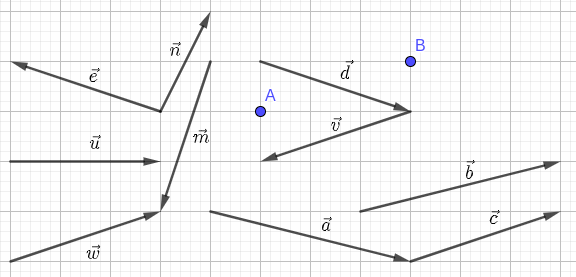
\includegraphics[width=0.7\textwidth]{./cap_vetor/dados/fig_exer_definicao_01/fig_exer_definicao_01}
  \end{figure}
\end{exer}
\begin{resp}
  $\vec{w}, \vec{c}$
\end{resp}

\begin{exer}
  Sejam $A$, $B$ e $C$ pontos dois a dois distintos. Se $\vec{b}$ é um vetor nulo, então $\vec{b}$ é igual a:
  \begin{enumerate}[a)]
  \item $\vec{0}$
  \item $\overrightarrow{AB}$
  \item $\overrightarrow{CC}$
  \item $\overrightarrow{CA}$
  \item $\overrightarrow{BB}$
  \end{enumerate}
\end{exer}
\begin{resp}
  a), c), e) 
\end{resp}

\begin{exer}
  Com base na figura abaixo, qual(is) dos vetores indicados são paralelos entre si.
  \begin{figure}[H]
    \centering
    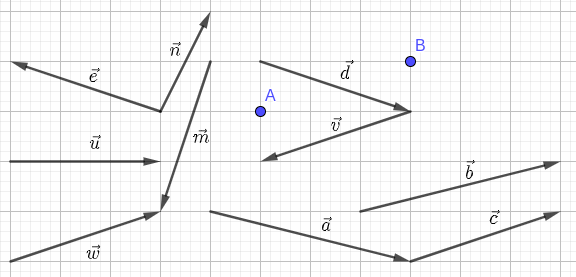
\includegraphics[width=0.7\textwidth]{./cap_vetor/dados/fig_exer_definicao_01/fig_exer_definicao_01}
  \end{figure}
\end{exer}
\begin{resp}
  $\vec{a}\parallel\vec{d}\parallel\vec{e}$; $\vec{c}\parallel\vec{v}\parallel\vec{w}$
\end{resp}

\begin{exer}
  Com base na figura abaixo, qual(is) dos vetores indicados são ortogonais (perpendiculares) entre si.
  \begin{figure}[H]
    \centering
    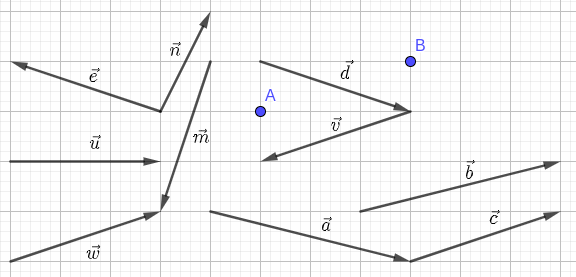
\includegraphics[width=0.7\textwidth]{./cap_vetor/dados/fig_exer_definicao_01/fig_exer_definicao_01}
  \end{figure}
\end{exer}
\begin{resp}
  $\vec{e}\perp\vec{n}$
\end{resp}

\begin{exer}
  Com base na figura abaixo, qual(is) dos seguintes são representações do vetor $\overrightarrow{v}+\overrightarrow{u}$?
  \begin{enumerate}[a)]
  \item $\overrightarrow{JG}$
  \item $\overrightarrow{QN}$
  \item $\overrightarrow{AD}$
  \item $\overrightarrow{JV}$
  \item $\overrightarrow{NN}$
  \end{enumerate}
  \begin{figure}[H]
    \centering
    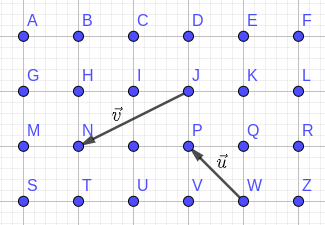
\includegraphics[width=0.7\textwidth]{./cap_vetor/dados/fig_exer_op_basicas/fig_vec_soma}
  \end{figure}
\end{exer}
\begin{resp}
  a), b)
\end{resp}

\begin{exer}
  Com base na figura abaixo, qual(is) dos seguintes são representações do vetor $\vec{w}+\vec{v}-\vec{u}$?
  \begin{enumerate}[a)]
  \item $\overrightarrow{0}$
  \item $\overrightarrow{SP}$
  \item $\overrightarrow{FP}$
  \item $\overrightarrow{v}$
  \item $\overrightarrow{AD}$
  \end{enumerate}
  \begin{figure}[H]
    \centering
    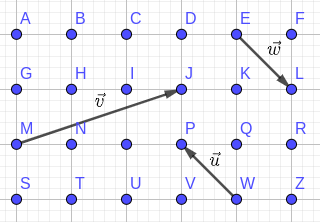
\includegraphics[width=0.7\textwidth]{./cap_vetor/dados/fig_exer_op_basicas/fig_vec_assop}
  \end{figure}
\end{exer}
\begin{resp}
  b), d)
\end{resp}

\begin{exer}
  Com base na figura abaixo, forneça o resultado das seguintes operações:
  \begin{enumerate}[a)]
  \item $\vec{u}-\vec{w}$
  \item $\vec{v}-\vec{u}$
  \item $\vec{a}+\vec{w}$
  \item $\vec{w}-\vec{a}-\vec{u}$
  \item $\vec{a}-\vec{v}$
  \end{enumerate}
  \begin{figure}[H]
    \centering
    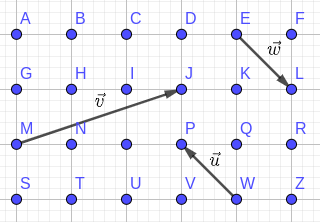
\includegraphics[width=0.7\textwidth]{./cap_vetor/dados/fig_exer_op_basicas/fig_vec_assop}
  \end{figure}
\end{exer}
\begin{resp}
  a)~$\vec{0}$; b)~$\overrightarrow{MQ}$; c)~$\overrightarrow{DZ}$; d)~$\overrightarrow{CD}$; e)~$\overrightarrow{DT}$
\end{resp}

\begin{exer}
  Com base na figura abaixo, escreva os seguintes vetores como resultado de operações envolvendo $\vec{u}$ ou $\vec{v}$.
  \begin{enumerate}[a)]
  \item $\overrightarrow{QK}$
  \item $\overrightarrow{KI}$
  \item $\overrightarrow{TO}$
  \item $\overrightarrow{PE}$
  \item $\overrightarrow{FT}$
  \end{enumerate}
  \begin{figure}[H]
    \centering
    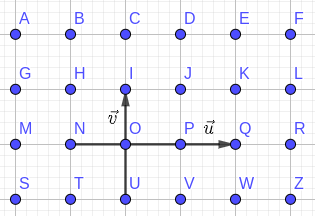
\includegraphics[width=0.7\textwidth]{./cap_vetor/dados/fig_exer_op_basicas/fig_vec_comb}
  \end{figure}
\end{exer}
\begin{resp}
  a)~$\frac{1}{2}\vec{v}$; b)~$-\frac{2}{3}\vec{u}$; c)~$\frac{1}{2}\vec{v}+\frac{1}{2}\vec{u}$; d)~$\vec{v}+\frac{1}{3}\vec{u}$; e)~$-\frac{4}{3}\vec{u}-\frac{3}{2}\vec{v}$
\end{resp}


\begin{exer}
  Seja dado um vetor $\vec{u}\neq 0$. Calcule a norma do vetor $\vec{v}=\vec{u}/|\vec{u}|$\footnote{$\vec{u}/|\vec{u}|$ é chamado de vetor $\vec{u}$ normalizado, ou a normalização do vetor $\vec{u}$.}.
\end{exer}
\begin{resp}
  $|\vec{v}|=1$.
\end{resp}

\begin{exer}
  Diga se é verdadeira ou falsa cada uma das seguintes afirmações. Justifique sua resposta.
  \begin{enumerate}
  \item $\vec{u}+\vec{u} = 2\vec{u}$
  \item $\vec{u}=-\vec{u} \Leftrightarrow \vec{u} = \vec{0}$.
  \end{enumerate}
\end{exer}
\begin{resp}
  a) verdadeira; b) verdadeira.
\end{resp}

%Este trabalho está licenciado sob a Licença Atribuição-CompartilhaIgual 4.0 Internacional Creative Commons. Para visualizar uma cópia desta licença, visite http://creativecommons.org/licenses/by-sa/4.0/deed.pt_BR ou mande uma carta para Creative Commons, PO Box 1866, Mountain View, CA 94042, USA.

\chapter{Bases e coordenadas}\label{cap_base}
\thispagestyle{fancy}

\section{Dependência linear}\label{cap_base_sec_deplinear}

\subsection{Combinação linear}

Dados vetores $\vec{u}_1$, $\vec{u}_2$, $\dotsc$, $\vec{u}_n$ e números reais $c_1$, $c_2$, $\dotsc$, $c_n$, com $n$ inteiro positivo, chamamos de
\begin{equation}
  \vec{u} = c_1\vec{u}_1 + c_2\vec{u}_2 + \cdots + c_n\vec{u}_n
\end{equation}
uma {\bf combinação linear}\index{combinação linear} de $\vec{u}_1$, $\vec{u}_2$, $\dotsc$, $\vec{u}_n$. Neste caso, também dizemos que $\vec{u}$ é {\bf gerado} pelos vetores $\vec{u}_1$, $\vec{u}_2$, $\dotsc$, $\vec{u}_n$ ou, equivalentemente, que estes vetores {\bf geram} o vetor $\vec{u}$.

\begin{ex}\label{ex:comblinear}
  Sejam dados os vetores $\vec{v}$, $\vec{w}$ e $\vec{z}$. Então, temos:
  \begin{itemize}
  \item $\vec{u}_1 = \frac{1}{2}\vec{u} + \sqrt{2}\vec{z}$ é uma combinação linear dos vetores $\vec{v}$ e $\vec{z}$.
  \item $\vec{u_2} = \vec{u} - 2\vec{z}$ é uma outra combinação linear dos vetores $\vec{v}$ e $\vec{z}$.
  \item $\vec{u_3} = 2\vec{u} - \vec{w} + \pi\vec{z}$ é uma combinação linear dos vetores $\vec{u}$, $\vec{w}$ e $\vec{z}$.
  \item $\vec{u_4} = \frac{3}{2}\vec{z}$ é uma combinação linear do vetor $\vec{z}$.
  \end{itemize}
\end{ex}

\subsection{Dependência linear}

Dois ou mais vetores dados são {\bf linearmente dependentes}\index{linearmente!dependente} (abreviação, l.d.) quando um deles for combinação linear dos demais.

\begin{ex}\label{ex:deplinear}
  No exemplo anterior (Exemplo \ref{ex:comlinear}), temos:
  \begin{itemize}
  \item $\vec{u_1}$ e $\vec{u_2}$ dependem linearmente dos vetores $\vec{u}$ e $\vec{z}$.
  \item $\vec{u_3}$ depende linearmente dos vetores $\vec{u}$, $\vec{v}$ e $\vec{z}$.
  \item Os vetores $\vec{u_4}$ e $\vec{z}$ são linearmente dependentes.
  \end{itemize}
\end{ex}

Dois ou mais vetores dados são {\bf linearmente independentes}\index{linearmente!independentes} (abreviação, l.i.)quando eles não são linearmente dependentes.

\subsection{Observações}

\subsubsection{Dois vetores}

Dois vetores quaisquer $\vec{u}\neq\vec{0}$ e $\vec{v}\neq\vec{0}$ são l.d. se, e somente se, qualquer uma das seguinte condições é satisfeita:
\begin{itemize}
\item um deles é combinação linear do outro, i.e.
  \begin{equation}
    \vec{u} = \alpha\vec{v}\quad\text{ou}\quad\vec{v}=\beta\vec{u};
  \end{equation}
\item $\vec{u}$ e $\vec{v}$ têm a mesma direção;
\item $\vec{u}$ e $\vec{v}$ são paralelos.
\end{itemize}

\begin{obs}
  O vetor nulo $\vec{0}$ é l.d. a qualquer vetor $\vec{u}$. De fato, temos
  \begin{equation}
    \vec{0} = 0\cdot\vec{u},
  \end{equation}
  i.e. o vetor nulo é combinação linear do vetor $\vec{u}$.
\end{obs}

\begin{obs}
  Dois vetores não nulos $\vec{u}$ e $\vec{v}$ são l.i. se, e somente se,
  \begin{equation}
    \alpha\vec{u} + \beta\vec{v} = 0 \Rightarrow \alpha=\beta=0.
  \end{equation}
  De fato, se $\alpha\neq 0$, então podemos escrever
  \begin{equation}
    \vec{u} = -\frac{\beta}{\alpha}\vec{v},
  \end{equation}
  i.e. o vetor $\vec{u}$ é combinação linear do vetor $\vec{v}$ e, portanto, estes vetores são l.d.. Isto contradiz a hipótese de eles serem l.i.. Analogamente, se $\beta \neq 0$, então podemos escrever
  \begin{equation}
    \vec{v} = -\frac{\alpha}{\beta}\vec{u}
  \end{equation}
  e, então, teríamos $\vec{u}$ e $\vec{v}$ l.d..
\end{obs}


\subsubsection{Três vetores}

Três vetores quaisquer $\vec{u}$, $\vec{v}$ e $\vec{w}$ são l.d. quando um deles pode ser escrito como combinação linear dois outros dois. Sem perda de generalidade, isto significa que existem constantes $\alpha$ e $\beta$ tais que
\begin{equation}
  \vec{u} = \alpha\vec{v} + \beta\vec{w}.
\end{equation}

Afirmamos que se $\vec{u}$, $\vec{v}$ e $\vec{w}$ são l.d., então $\vec{u}$, $\vec{v}$ e $\vec{w}$ são coplanares. Do fato de que dois vetores quaisquer são sempre coplanares, temos que $\vec{u}$, $\vec{v}$ e $\vec{w}$ são coplanares caso qualquer um deles seja o vetor nulo. Suponhamos, agora, que $\vec{u}$, $\vec{v}$ e $\vec{w}$ são não nulos e seja $\pi$ o plano determinado pelos vetores $\vec{v}$ e $\vec{w}$. Se $\alpha = 0$, então $\vec{u} = \beta\vec{w}$ e teríamos uma representação de $\vec{u}$ no plano $\pi$. Analogamente, se $\beta=0$, então $\vec{u} = \alpha\vec{v}$ e teríamos uma representação de $\vec{u}$ no plano $\pi$. Por fim, observemos que se $\alpha,\beta\neq 0$, então $\alpha\vec{v}$ tem a mesma direção de $\vec{v}$ e $\beta\vec{w}$ tem a mesma direção de $\vec{w}$. Isto é, $\alpha\vec{v}$ e $\beta\vec{w}$ admitem representações no plano $\pi$. Sejam $\overrightarrow{AB}$ e $\overrightarrow{BC}$ representações dos vetores $\alpha\vec{v}$ e $\beta\vec{w}$, respectivamente. Os pontos $A$, $B$ e $C$ pertencem a $\pi$, assim como o segmento $AC$. Como $\overrightarrow{AC} = \vec{u} = \alpha\vec{v} + \beta\vec{w}$, concluímos que $\vec{u}$, $\vec{v}$ e $\vec{w}$ são coplanares.

Reciprocamente, se $\vec{u}$, $\vec{v}$ e $\vec{w}$ são coplanares, então $\vec{u}$, $\vec{v}$ e $\vec{w}$ são l.d.. De fato, se um deles for nulo, por exemplo, $\vec{u}=\vec{0}$, então $\vec{u}$ pode ser escrito como a seguinte combinação linear dos vetores $\vec{v}$ e $\vec{w}$
\begin{equation}
  \vec{u} = 0\vec{v} + 0\vec{w}.
\end{equation}
Neste caso, $\vec{u}$, $\vec{v}$ e $\vec{w}$ são l.d.. Também, se dois dos vetores forem paralelos, por exemplo, $\vec{u}\parallel\vec{v}$, então temos a combinação linear
\begin{equation}
  \vec{u} = \alpha\vec{v} + 0\vec{w}.
\end{equation}
E, então, $\vec{u}$, $\vec{v}$ e $\vec{w}$ são l.d.. Agora, suponhamos que $\vec{u}$, $\vec{v}$ e $\vec{w}$ são não nulos e dois a dois concorrentes. Sejam, então $\overrightarrow{PA}=\vec{u}$, $\overrightarrow{PB}=\vec{v}$ e $\overrightarrow{PC}=\vec{w}$ representações sobre um plano $\pi$. Sejam $r$ e $s$ as retas determinadas por $PA$ e $PC$, respectivamente. Seja, então, $D$ o ponto de interseção da reta $s$ com a reta paralela a $r$ que passa pelo ponto $B$. Seja, também, $E$ o ponto de interseção da reta $r$ com a reta paralela a $s$ que passa pelo ponto $B$. Sejam, então, $\alpha$ e $\beta$ tais que $\alpha\vec{u}=\overrightarrow{PE}$ e $\beta\vec{w}=\overrightarrow{PD}$. Como $\vec{v} = \overrightarrow{PB} = \overrightarrow{PE} + \overrightarrow{PD} = \alpha\vec{u}+\beta\vec{w}$, temos que $\vec{v}$ é combinação linear de $\vec{u}$ e $\vec{w}$, i.e. $\vec{u}$, $\vec{v}$ e $\vec{w}$ são l.d..

\begin{obs}
  Três vetores dados $\vec{u}$, $\vec{v}$ e $\vec{w}$ são l.i. se, e somente se, 
  \begin{equation}
    \alpha\vec{u} + \beta\vec{v} + \gamma\vec{w} = 0 \Rightarrow \alpha=\beta=\gamma = 0.
  \end{equation}
  De fator, sem perda de generalidade, se $\alpha\neq 0$, podemos escrever
  \begin{equation}
    \vec{u} = -\frac{\beta}{\alpha}\vec{v} - \frac{\gamma}{\alpha}\vec{w},
  \end{equation}
  e teríamos $\vec{u}$, $\vec{v}$ e $\vec{w}$ vetores l.d..
\end{obs}

\subsubsection{Quatro ou mais vetores}

{\bf Quatro ou mais vetores são sempre l.d..} De fato, sejam dados quatro vetores $\vec{a}$, $\vec{b}$, $\vec{c}$ e $\vec{d}$. Se dois ou três destes forem l.d. entre si, então, por definição, os quatro são l.d.. Assim sendo, suponhamos que três dos vetores sejam l.i. e provaremos que, então, o outro vetor é combinação linear desses três.

Sem perda de generalidade, suponhamos que $\vec{a}$, $\vec{b}$ e $\vec{c}$ são l.i.. Logo, eles não são coplanares. Seja, ainda, $\pi$ o plano determinado pelos vetores $\vec{a}$, $\vec{b}$ e as representações $\vec{a}=\overrightarrow{PA}$, $\vec{b}=\overrightarrow{PB}$, $\vec{c}=\overrightarrow{PC}$ e $\vec{d}=\overrightarrow{PD}$.

\begin{figure}[H]
  \centering
  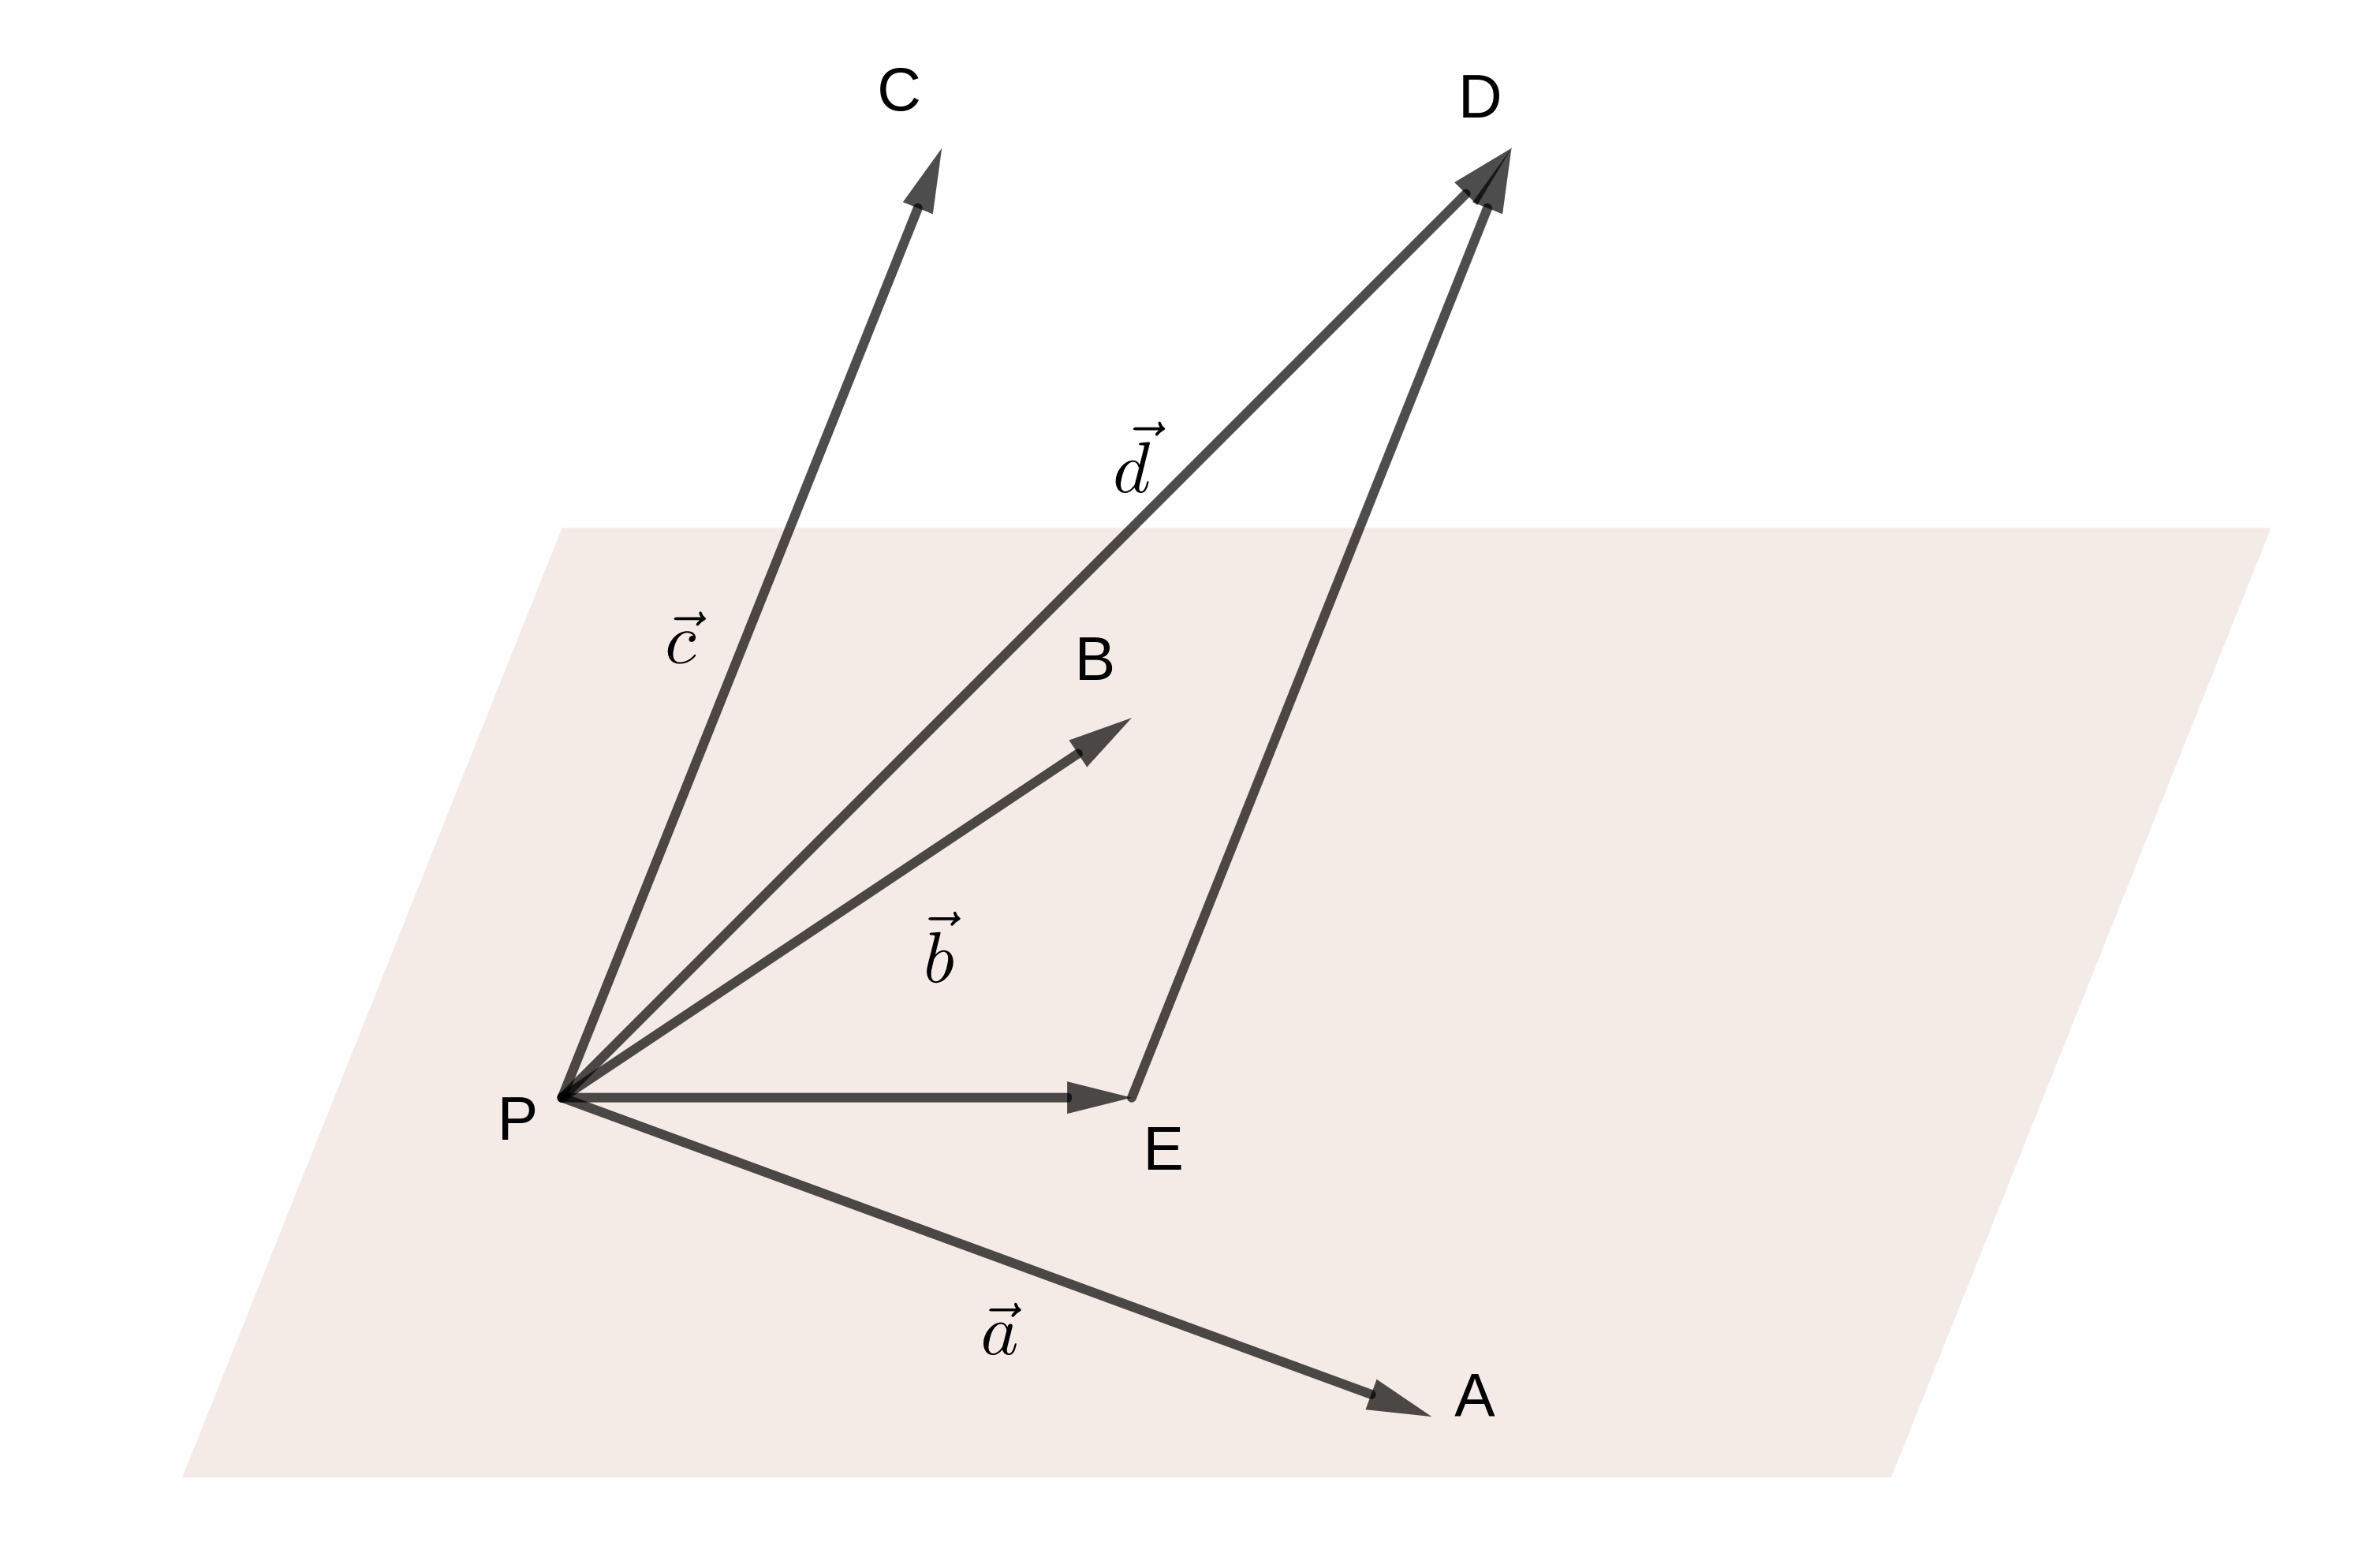
\includegraphics[width=0.7\textwidth]{./cap_base/dados/fig_4vec_ld/fig_4vec_ld}
  \caption{Quatro vetores são l.d..}
  \label{fig:4vec_ld}
\end{figure}

Consideremos a reta $r$ paralela a $\overrightarrow{PC}$ que passa pelo ponto $D$. Então, seja $E$ o ponto de interseção de $r$ com o plano $\pi$. Vejamos a Figura \ref{fig:}. Observamos que o vetor $\overrightarrow{PE}$ é coplanar aos vetores $\overrightarrow{PA}$ e $\overrightarrow{PB}$ e, portanto, exitem números reais $alpha$ e $\beta$ tal que
\begin{equation}
  \overrightarrow{PE} = \alpha\overrightarrow{PA} + \beta\overrightarrow{PB}.
\end{equation}
Além disso, como $\overrightarrow{ED}$ tem a mesma direção e sentido de $\overrightarrow{PC} = \vec{c}$, temos que
\begin{equation}
  \overrightarrow{ED} = \gamma\overrightarrow{PC}
\end{equation}
para algum número real $\gamma$. Por fim, observamos que
\begin{align*}
  \overrightarrow{PD} &= \overrightarrow{PE} + \overrightarrow{ED}\\
                      &= \alpha\overrightarrow{PA} + \beta\overrightarrow{PB} + \gamma\overrightarrow{PC}\\
                      &= \alpha\vec{a} + \beta\vec{b} + \gamma\vec{c}.
\end{align*}

\subsection*{Exercícios}

\emconstrucao

%Este trabalho está licenciado sob a Licença Atribuição-CompartilhaIgual 4.0 Internacional Creative Commons. Para visualizar uma cópia desta licença, visite http://creativecommons.org/licenses/by-sa/4.0/deed.pt_BR ou mande uma carta para Creative Commons, PO Box 1866, Mountain View, CA 94042, USA.

\chapter{Produto escalar}\label{cap_prodesc}
\thispagestyle{fancy}

\section{Produto escalar}\label{cap_prodesc_sec_prodesc}

Ao longo desta seção, assumiremos $B = (\vec{i},\vec{j},\vec{k})$ uma base ortonormal no espaço. O {\bf produto escalar} dos vetores $\vec{u} = (u_1,u_2,u_3)$ e $\vec{v}=(v_1,v_2,v_3)$ é o número real
\begin{equation}
  \vec{u}\cdot\vec{v} = u_1v_1+u_2v_2+u_3v_3.
\end{equation}

\begin{ex}
  Se $\vec{u}=(2,-1,3)$ e $\vec{v}=(-3,-4,2)$, então
  \begin{equation}
    \vec{u}\cdot\vec{v} = 2\cdot(-3)+(-1)\cdot(-4)+3\cdot 2 = 4.
  \end{equation}
\end{ex}

\subsection{Propriedades do produto interno}

Quaisquer que sejam $\vec{u}$, $\vec{v}$, $\vec{w}$ e qualquer número real $\alpha$, temos:
\begin{itemize}
\item Comutatividade: $\vec{u}\cdot\vec{v}=\vec{v}\cdot\vec{u}$.

  Dem.:
  \begin{align}
    \vec{u}\cdot\vec{v} &= (u_1,u_2,u_3)\cdot(v_1,v_2,v_3)\\
                        &= u_1v_1+u_2v_2+u_3v_3 \\
                        &= v_1u_1+v_2u_2+v_3u_3 \\
                        &= \vec{v}\cdot\vec{u}.
  \end{align}

\item Distributividade com multiplicação por escalar:
  \begin{equation}
  (\alpha\vec{u})\cdot\vec{v}=\vec{u}\cdot(\alpha\vec{v})=\alpha(\vec{u}\cdot\vec{v}).
\end{equation}


  Dem.:
  \begin{align}
    (\alpha\vec{u})\cdot\vec{v} &= (\alpha u_1,\alpha u_2, \alpha u_3)\cdot (v_1,v_2,v_3)\\
                                &= (\alpha u_1)v_1+(\alpha u_2)v_2 + (\alpha u_3)v_3 \\
                                &= \alpha (u_1v_1)+\alpha (u_2v_2)+\alpha (u_3v_3) \\
                                &= \alpha (u_1v_1+u_2v_2+u_3v_3) = \alpha(\vec{u}\cdot\vec{v})\\
                                &= u_1(\alpha v_1) + u_2(\alpha v_2) + u_3(\alpha v_3) \\
                                &= (u_1,u_2,u_3)\cdot(\alpha v_1,\alpha v_2,\alpha v_3) \\
                                &= \vec{u}\cdot(\alpha\vec{v}).
  \end{align}

\item Distributividade com a adição: $\vec{u}\cdot(\vec{v}+\vec{w}) = \vec{u}\cdot\vec{v}+\vec{u}\cdot\vec{w}$.

  Dem.:
  \begin{align}
    \vec{u}\cdot(\vec{v}+\vec{w}) &= (u_1,u_2,u_3)\cdot\left((v_1,v_2,v_3)+(w_1,w_2,w_3)\right) \\
                                  &= (u_1,u_2,u_3)\cdot [(v_1+w_1,v_2+w_2,v_3+w_3)] \\
                                  &= u_1(v_1+w_1) + u_2(v_2+w_2) + u_2(v_2+w_2) \\
                                  &= u_1v_1+u_1w_1+u_2v_2+u_2w_2+u_3v_3+u_3w_3 \\
                                  &= u_1v_1+u_2v_2+u_3v_3 + u_1w_1+u_2w_2+u_3w_3 \\
                                  &= \vec{u}\cdot\vec{v}+\vec{u}\cdot\vec{w}.
  \end{align}

\item Sinal: $\vec{u}\cdot\vec{u}\geq 0$ e $\vec{u}\cdot\vec{u}=0 \Leftrightarrow \vec{u}=\vec{0}$.

  Dem.:
  \begin{align}
    \vec{u}\cdot\vec{u} = u_1^2+u_2^2+u_3^2 \geq 0.
  \end{align}
  Além disso, observamos que a soma de números não negativos é nula se, e somente se, os números forem zeros.

\item Norma: $|u|^2 = \vec{u}\vec{u}$.

  Dem.:
  Como fixamos uma base ortonormal $B$, a Proposição \ref{prop:bo_norma} nos garante que
  \begin{equation}
    |u|^2 = u_1^2+u_2^2+u_3^2 = \vec{u}\cdot\vec{u}.
  \end{equation}
\end{itemize}

\begin{ex}
  Sejam $\vec{u}=(-1,2,1)$, $\vec{v}=(2,-1,3)$ e $\vec{w}=(1,0,-1)$. Vejamos os seguintes casos:
  \begin{itemize}
  \item Comutatividade:
    \begin{align}
      \vec{u}\cdot\vec{v} &= -1\cdot 2 + 2\cdot (-1) + 1\cdot 3 = -1,\\
      \vec{v}\cdot\vec{u} &= 2\cdot(-1) + (-1)\cdot 2 + 3\cdot 1 = -1.            
    \end{align}
  \item Distributividade com a multiplicação por escalar:
    \begin{align}
      (2\vec{u})\cdot\vec{v} &= (-2,4,2)\cdot(2,-1,3) = -4-4+6=-2,\\
      2(\vec{u}\vec{v}) &= 2(-2-2+3) = -2,\\
      \vec{u}\cdot(2\vec{v}) &= (-1,2,1)\cdot(4,-2,6) = -2.
    \end{align}
  \item Distributividade com a adição:
    \begin{align}
      \vec{u}\cdot(\vec{v}+\vec{w})) &= (-1,2,1)\cdot(3,-1,2) = -3-2+2=-3,\\
      \vec{u}\cdot\vec{v}+\vec{u}\cdot\vec{w} &= (-2-2+3)+(-1+0-1) = -3.
    \end{align}
  \item Sinal:
    \begin{align}
      \vec{w}\vec{w} = 1+0+1 = 2 \geq 0.
    \end{align}
  \item Norma:
    \begin{align}
      |u|^2 &= (-1)^2+2^2+1^2 = 6,\\
      \vec{u}\cdot\vec{u} &= (-1)\cdot(-1)+2\cdot 2+1\cdot 1 = 6.
    \end{align}
  \end{itemize}
\end{ex}

\subsection{Ângulo entre dois vetores}

O {\bf ângulo formado entre dois vetores} $\vec{u}$ e $\vec{v}$ não nulos, é definido como o menor ângulo determinado entre quaisquer representações $\vec{u} = \overrightarrow{OA}$ e $\vec{v} = \overrightarrow{OB}$.

\begin{prop}\label{prop:angulo_prodesc}
  Dados $\vec{u}$ e $\vec{v}$, temos
  \begin{equation}
    \vec{u}\cdot\vec{v}=|\vec{u}||\vec{v}|\cos\alpha,
  \end{equation}
  onde $\alpha$ é o ângulo entre os vetores $\vec{u}$ e $\vec{v}$.
\end{prop}
\begin{dem}
  Tomamos as representações $\vec{u} = \overrightarrow{OA}$ e $\vec{v} = \overrightarrow{OB}$. Observamos que $\vec{u}-\vec{v} = \overrightarrow{BA}$. Então, aplicando a lei dos cossenos no triângulo $\triangle OAB$, obtemos
  \begin{equation}
    |\overrightarrow{BA}|^2 = |\overrightarrow{OA}|^2 + |\overrightarrow{OB}|^2 - 2|\overrightarrow{OA}||\overrightarrow{OB}|\cos\alpha,
  \end{equation}
  ou, equivalentemente,
  \begin{align}
    |\vec{u}-\vec{v}|^2 &= |\vec{u}|^2+|\vec{v}|^2-2|\vec{u}||\vec{v}|\cos\alpha\\
    (\vec{u}-\vec{v})\cdot(\vec{u}-\vec{v}) &= |\vec{u}|^2+|\vec{v}|^2-2|\vec{u}||\vec{v}|\cos\alpha\\
    \vec{u}\cdot\vec{u}-2\vec{u}\cdot\vec{v}+\vec{v}\cdot\vec{v} &= |\vec{u}|^2+|\vec{v}|^2-2|\vec{u}||\vec{v}|\cos\alpha\\
    |\vec{u}|^2+|\vec{v}|^2-2\vec{u}\cdot\vec{v} &= |\vec{u}|^2+|\vec{v}|^2-2|\vec{u}||\vec{v}|\cos\alpha
  \end{align}
  donde
  \begin{equation}
    \vec{u}\cdot\vec{v} = |\vec{u}||\vec{v}|\cos\alpha.
  \end{equation}
\end{dem}

\begin{ex}
  Vamos determinar ângulo entre os vetores $\displaystyle \vec{u}=\left(\frac{\sqrt{3}}{2},\frac{1}{2},0\right)$ e $\displaystyle \vec{u}=\left(\frac{1}{2},\frac{\sqrt{3}}{2},0\right)$. Da Proposição \ref{prop:angulo_prodesc}, temos
    \begin{align}
      \cos\alpha &= \frac{\vec{u}\cdot\vec{v}}{|u|\cdot|v|}\\
      &= \frac{\frac{\sqrt{3}}{2}}{1\cdot 1} = \frac{\sqrt{3}}{2}.
    \end{align}
    Portanto, temos $\alpha = \pi/6$.
\end{ex}

\subsection*{Exercícios}

\emconstrucao
%Este trabalho está licenciado sob a Licença Atribuição-CompartilhaIgual 4.0 Internacional Creative Commons. Para visualizar uma cópia desta licença, visite http://creativecommons.org/licenses/by-sa/4.0/deed.pt_BR ou mande uma carta para Creative Commons, PO Box 1866, Mountain View, CA 94042, USA.

\chapter{Produto vetorial}\label{cap_prodvet}
\thispagestyle{fancy}

De agora em diante, vamos trabalhar com um base ortonormal $B = (\vec{i}, \vec{j}, \vec{k})$ dita com orientação positiva, i.e. os vetores $\vec{i} = \overrightarrow{OI}$, $\vec{j} = \overrightarrow{OJ}$ e $\vec{k}=\overrightarrow{OK}$ estão dispostos em sentido anti-horário, veja Figura \ref{fig:base_pos}.

\begin{figure}[H]
  \centering
  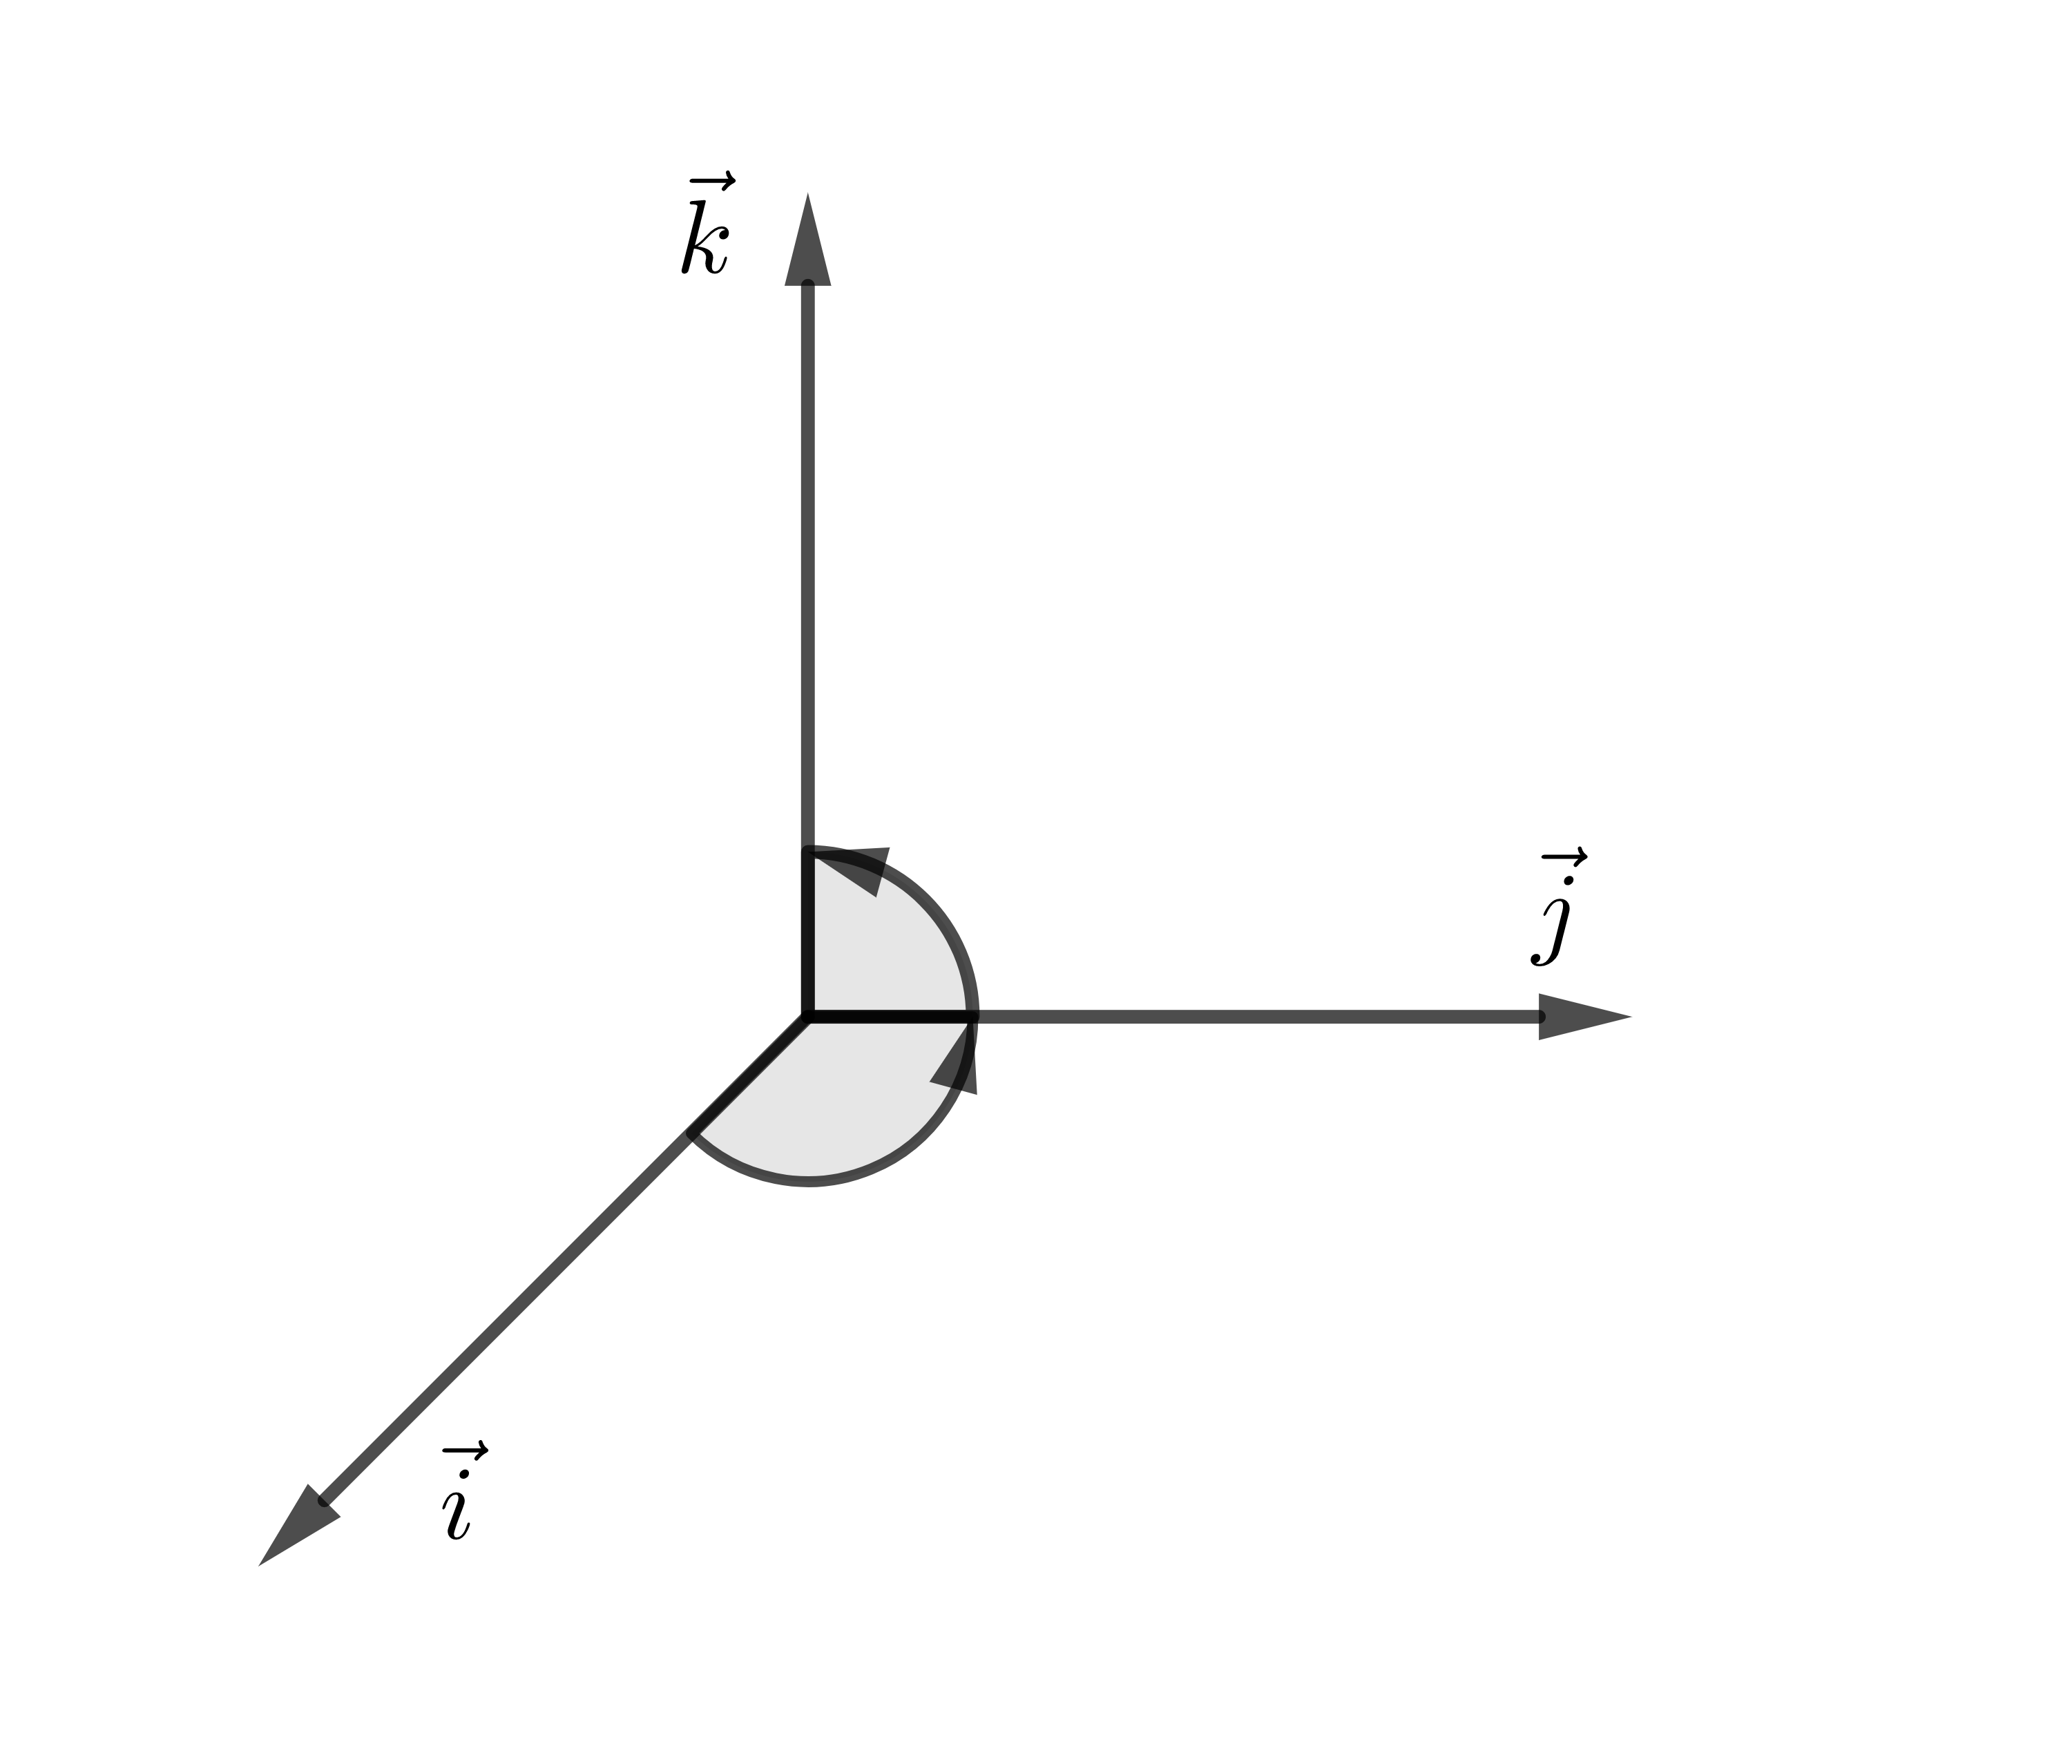
\includegraphics[width=0.7\textwidth]{./cap_prodvet/dados/fig_base_pos/fig_base_pos}
  \caption{Base ortonormal positiva.}
  \label{fig:base_pos}
\end{figure}

\section{Definição}\label{cap_prodvet_sec_prodvet}

Dados vetores $\vec{u}$ e $\vec{v}$, definimos o produto vetorial de $\vec{u}$ com $\vec{v}$, denotado por $\vec{u}\land\vec{v}$, como o vetor:
\begin{itemize}
\item se $\vec{u}$ e $\vec{v}$ são l.d., então $\vec{u}\land\vec{v} = \vec{0}$.
\item se $\vec{u}$ e $\vec{v}$ são l.i., então
  \begin{itemize}
  \item $|\vec{u}\land\vec{v}| = |\vec{u}||\vec{v}|\sen\alpha$, onde $\alpha$ é o ângulo entre $\vec{u}$ e $\vec{v}$,
  \item $\vec{u}\land\vec{v}$ é ortogonal a $\vec{u}$ e $\vec{v}$, e
  \item $\vec{u}$, $\vec{v}$ e $\vec{u}\land\vec{v}$ formam uma base positiva.
  \end{itemize}
\end{itemize}

\subsection{Interpretação geométrica}

Sejam dados $\vec{u}$ e $\vec{v}$ l.i.. Estes vetores determinam um paralelogramo, veja Figura \ref{fig:prodvet_interp} (esquerda). Seja, então, $h$ a altura deste paralelogramo tendo $\vec{u}$ como sua base. Logo, a área do paralelogramo é o produto do comprimento da base com sua altura, neste caso
\begin{align}
  |\vec{u}|h &= |\vec{u}||\vec{v}|\sen\alpha\\
             &= |\vec{u}\land\vec{v}|
\end{align}
Ou seja, o produto vetorial $\vec{u}\land\vec{v}$ tem norma igual à área do paralelogramo determinado por $\vec{u}$ e $\vec{v}$.

Ainda, por definição, $\vec{u}\land\vec{v}$ é ortogonal a $\vec{u}$ e $\vec{v}$. Isto nos dá a direção de $\vec{u}\land\vec{v}$. O sentido é, então, determinado pela definição de que $(\vec{u},\vec{v},\vec{u}\land\vec{v})$ é uma base positiva. Veja a Figura \ref{fig:prodvet_interp} (direita).

\begin{figure}[H]
  \centering
  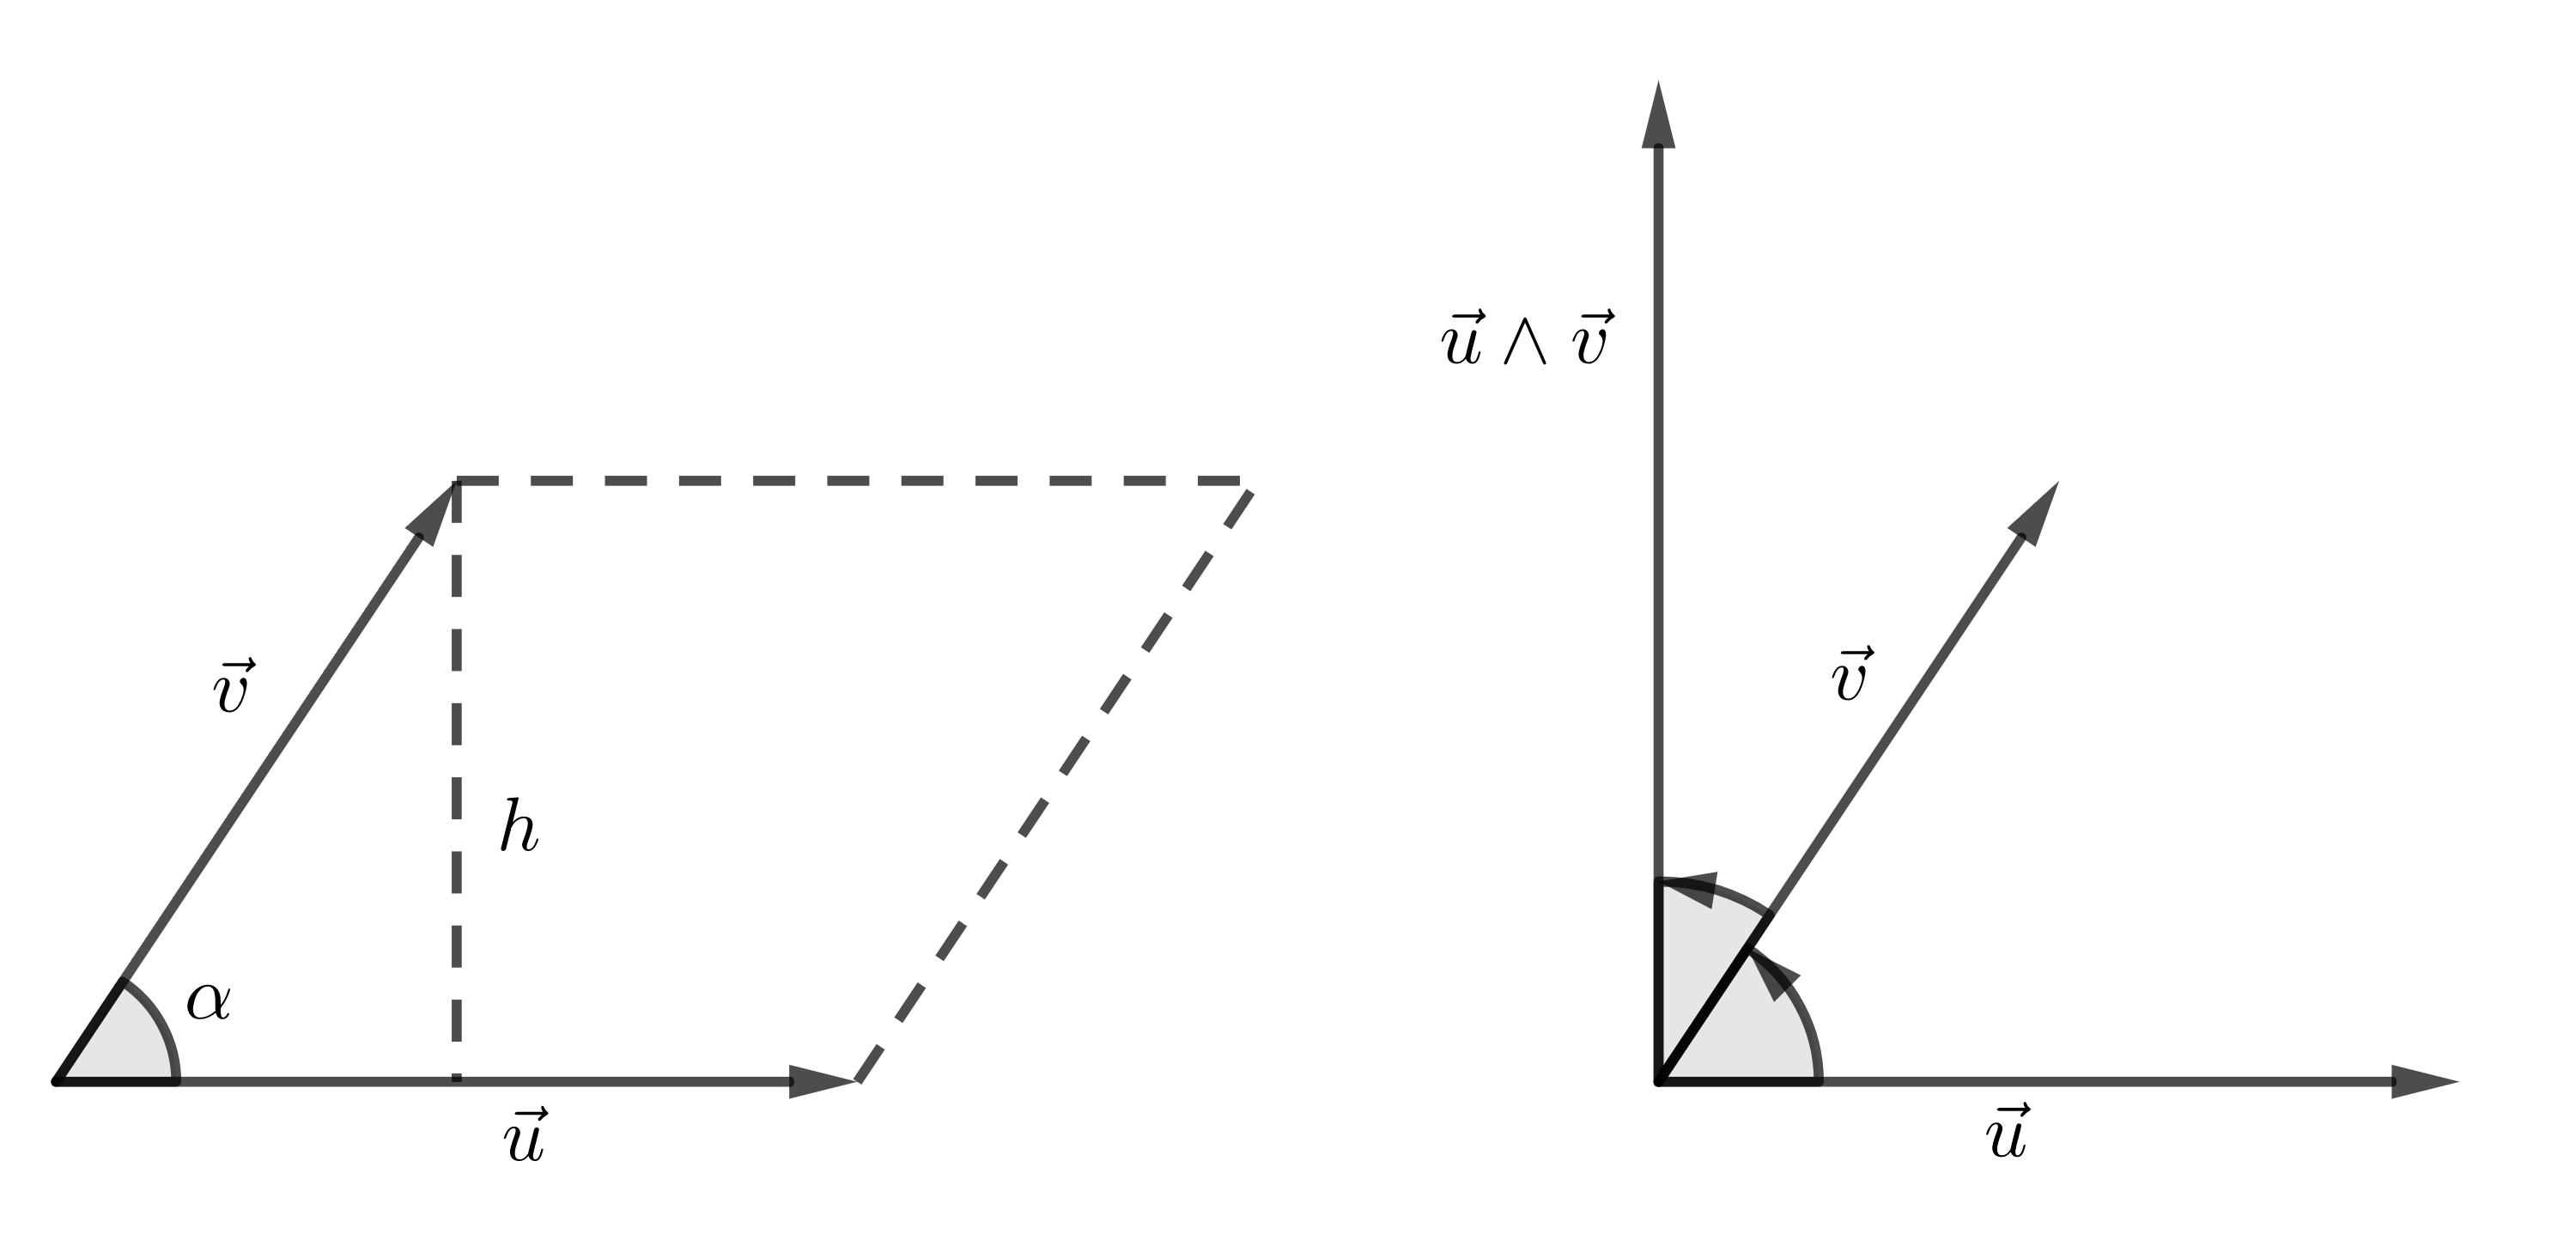
\includegraphics[width=0.7\textwidth]{./cap_prodvet/dados/fig_prodvet_interp/fig_prodvet_interp}
  \caption{Interpretação do produto vetorial.}
  \label{fig:prodvet_interp}
\end{figure}

\subsection{Produto vetorial via coordenadas}\label{cap_prodvet_sec_coord}

Dados $\vec{u} = (u_1,u_2,u_3)$ e $\vec{v} = (v_1,v_2,v_3)$ em uma base ortonormal positiva, então
\begin{equation}
  \vec{u}\land\vec{v} =
  \begin{vmatrix}
    u_2 & u_3\\
    v_2 & v_3
  \end{vmatrix}\vec{i} -
  \begin{vmatrix}
    u_1 & u_3\\
    v_1 & v_3
  \end{vmatrix}\vec{j} +
  \begin{vmatrix}
    u_1 & u_2 \\
    v_1 & v_2
  \end{vmatrix}\vec{k}.
\end{equation}

\begin{obs}
  Uma regra mnemônica, é
  \begin{equation}
    \vec{u}\land\vec{v} =
    \begin{vmatrix}
      \vec{i} & \vec{j} & \vec{k} \\
      u_1 & u_2 & u_3 \\
      v_1 & v_2 & v_3
    \end{vmatrix}.
  \end{equation}
\end{obs}

\begin{ex}
  Dados os vetores $\vec{u} = (1,-2,1)$ e $\vec{v} = (0,2,-1)$, temos
  \begin{align}
    \vec{u}\land\vec{v} &=
                          \begin{vmatrix}
                            \vec{i} & \vec{j} & \vec{k} \\
                            u_1 & u_2 & u_3 \\
                            v_1 & v_2 & v_3
                          \end{vmatrix} \\
                        &=
                          \begin{vmatrix}
                            \vec{i} & \vec{j} & \vec{k} \\
                            1       & -2      & 1 \\
                            0       & 2       & -1
                          \end{vmatrix} \\
                        &= 0\vec{i} + \vec{j} + 2\vec{k}\\
                        &= (0,1,2).
  \end{align}
\end{ex}

\subsection*{Exercícios resolvidos}

\begin{exeresol}
  Calcule $\vec{x}$ tal que $(0,2,-1)\land\vec{x}=(-3,-1,-2)$.
\end{exeresol}
\begin{resol}
  Denotando $\vec{x}=(x_1,x_2,x_3)$, temos
  \begin{gather}
    (0,2,-1)\land\vec{x}=(-3,-1,-2)\\
    \begin{vmatrix}
      \vec{i} & \vec{j} & \vec{k} \\
      0 & 2 & -1 \\
      x_1 & x_2 & x_3
    \end{vmatrix} = (-3,-1,-2)\\
    (x_2+2x_3)\vec{i}-x_1\vec{j}-2x_1\vec{k} = \\
    -3\vec{i}-\vec{j}-2\vec{k}
  \end{gather}
  Segue que
  \begin{align*}
    x_2+2x_3 &= -3\\
    -x_1 &= -1\\
    -2x_1 &= -2
  \end{align*}
  Logo, $x_1 = 1$, $x_2=-3-2x_3$ e $x_3$ é arbitrário. Concluímos que $\vec{x} = (1,-3-2x_3,x_3)$ com $x_3\in\mathbb{R}$.
\end{resol}

\begin{exeresol}
  Determine a área do paralelogramo determinado pelos vetores $\vec{u} = (-1, 2, 3)$ e $\vec{v} = (1,-2,1)$.
\end{exeresol}
\begin{resol}
  Tomando representações $\vec{u}=\overrightarrow{OA}$ e $\vec{v}=\overrightarrow{OC}$, temos que $\vec{u}$ e $\vec{v}$ determinam um paralelogramo $OABC$, onde $C$ é tal que $\vec{u}+\vec{v}=\overrightarrow{OB}$\footnote{Veja a regra do paralelogramo na Observação \ref{obs:vetor_regra_do_paralelogramo}.}. Da definição do produto vetorial, temos que
  \begin{equation}
    |\vec{u}\land\vec{v}| = |\vec{u}||\vec{v}|\sen\alpha,
  \end{equation}
  o que é igual a área do paralelogramo $OABC$, onde $\alpha$ é o ângulo entre os vetores $\vec{u}$ e $\vec{v}$. Logo, a área do paralelogramo é
  \begin{gather}
    |\vec{u}\land\vec{v}| =
    \begin{vmatrix}
      \vec{i} & \vec{j} & \vec{k} \\
      -1 & 2 & 3 \\
      1 & -2 & 1
    \end{vmatrix}\\
    |\vec{u}\land\vec{v}| = |(8,4,0)|\\
    |\vec{u}\land\vec{v}| = 4\sqrt{5}
  \end{gather}
\end{resol}

\subsection*{Exercícios}

\begin{exer}
  Sejam $\vec{u}=(2,-3,1)$ e $\vec{v}=(1,-2,-1)$. Calcule:
  \begin{enumerate}[a)]
  \item $\vec{u}\land\vec{v}$.
  \item $\vec{v}\land\vec{u}$.
  \item $\vec{v}\land(2\vec{u})$.
  \end{enumerate}
\end{exer}
\begin{resp}
  a)~$(5,3,-1)$; b)~$(-5,-3,1)$; c)~$(-10,-6,2)$
\end{resp}

\begin{exer}
  Sejam $\vec{u}$ e $\vec{v}$ tais que $\vec{u}\land\vec{v}=(2,-1,0)$. Forneça $\vec{v}\land\vec{u}$. Justifique sua resposta.
\end{exer}
\begin{resp}
  $(-2,1,0)$
\end{resp}

\begin{exer}
  Seja $\vec{u}$ um vetor qualquer. Calcule $\vec{u}\land\vec{u}$.
\end{exer}
\begin{resp}
  $0$
\end{resp}

\begin{exer}
  Sejam $\vec{u}$ e $\vec{v}$ tais que $(2\vec{u})\land\vec{v}=(2,-1,0)$. Forneça $\vec{v}\land\vec{u}$. Justifique sua resposta.
\end{exer}
\begin{resp}
  $(-1,1/2,0)$
\end{resp}

\begin{exer}
  Calcule $\vec{x}$ tal que $\vec{x}\land (2,-2,3)=(11,8,2)$.
\end{exer}
\begin{resp}
  $\left(-\frac{2}{3}x_3+\frac{8}{3},\frac{2}{3}x_3-\frac{11}{3},x_3\right), x_3\in\mathbb{R}$
\end{resp}

\begin{exer}
  Seja $B=(\vec{i},\vec{j},\vec{k})$ uma base ortonormal positiva. Calcule:
  \begin{enumerate}[a)]
  \item $\vec{i}\land\vec{j}$
  \item $\vec{j}\land\vec{k}$
  \item $\vec{k}\land\vec{i}$
  \end{enumerate}
\end{exer}
\begin{resp}
  a)~$\vec{k}$; b)~$\vec{i}$; c)~$\vec{j}$
\end{resp}

\section{Propriedades do produto vetorial}\label{cap_prodvet_sec_prop}

Nesta seção, discutiremos sobre algumas propriedades do produto vetorial. Para tanto, sejam dados os vetores $\vec{u} = (u_1,u_2,u_3)$, $\vec{v}=(v_1,v_2,v_3)$, $\vec{w}=(w_1,w_2,w_3)$ e o número real $\gamma$.

Da definição do produto vetorial, temos $\vec{u}\perp(\vec{u}\land\vec{v})$ e $\vec{v}\perp(\vec{u}\land\vec{v})$, logo
\begin{equation}
  {\color{blue}\vec{u}\cdot(\vec{u}\land\vec{v}) = 0}
\end{equation}
e
\begin{equation}
  {\color{blue}\vec{v}\cdot(\vec{u}\land\vec{v}) = 0}.
\end{equation}

\begin{ex}
  Sejam $\vec{u}=(1,-1,2)$, $\vec{v}=(2,-1,-2)$. Temos
  \begin{align}
    \vec{u}\land\vec{v} &=
    \begin{vmatrix}
      \vec{i} & \vec{j} & \vec{k} \\
      1 & -1 & 2 \\
      2 & -1 & -2
    \end{vmatrix}\\
              &= (4,6,1)
  \end{align}
  Segue, que
  \begin{align}
    \vec{u}\cdot(\vec{u}\land\vec{v}) &= (1,-1,2)\cdot (4,6,1) \\
                                      &= 4-6+2\\
                                      &= 0.
  \end{align}
\end{ex}

Em relação à multiplicação por escalar, temos
\begin{align}
  {\color{blue}\gamma(\vec{u}\land\vec{v})} &= {\color{red}(\gamma\vec{u})\land\vec{v}} \\
                              &= {\color{cyan}\vec{u}\land(\gamma\vec{v})}.
\end{align}
De fato,
\begin{align}
  {\color{red}(\gamma\vec{u})\land\vec{v}} &=
                                {\color{red}\begin{vmatrix}
                                  \vec{i} & \vec{j} & \vec{k} \\
                                  \gamma u_1 & \gamma u_2 & \gamma u_3\\
                                  v_1 & v_2 & v_3
                                \end{vmatrix}} \\
                              &= {\color{blue}\gamma\begin{vmatrix}
                                  \vec{i} & \vec{j} & \vec{k} \\
                                  u_1 & u_2 & u_3\\
                                  v_1 & v_2 & v_3
                                \end{vmatrix}} = {\color{blue}\gamma(\vec{u}\land\vec{v})}\\
                              &=
                                {\color{cyan}\begin{vmatrix}
                                  \vec{i} & \vec{j} & \vec{k} \\
                                  u_1 & u_2 & u_3\\
                                  \gamma v_1 & \gamma v_2 & \gamma v_3
                                \end{vmatrix}} = {\color{cyan}\vec{u}\land(\gamma\vec{v})}
\end{align}

\begin{ex}
  Sejam $\vec{u}=(1,-1,2)$ e $\vec{v}=(2,-1,-2)$. Temos
  \begin{align}
    {\color{blue}2(\vec{u}\land\vec{v})} &=
    2\begin{vmatrix}
      \vec{i} & \vec{j} & \vec{k} \\
      1 & -1 & 2 \\
      2 & -1 & -2
    \end{vmatrix}\\
                           &= 2(4,6,1)\\
                           &= (8,12,2)
  \end{align}
  \begin{align}
    {\color{red}(2\vec{u})\land\vec{v}} &=
    \begin{vmatrix}
      \vec{i} & \vec{j} & \vec{k} \\
      2 & -2 & 4 \\
      2 & -1 & -2
    \end{vmatrix}\\
                           &= (8,12,2)
  \end{align}
  \begin{align}
    {\color{cyan}\vec{u}\land(2\vec{v})} &=
    \begin{vmatrix}
      \vec{i} & \vec{j} & \vec{k} \\
      1 & -1 & 2 \\
      4 & -2 & -4
    \end{vmatrix}\\
                           &= (8,12,2)
  \end{align}
\end{ex}


Também, vale a {\color{blue}propriedade distributiva com a operação de soma}, i.e.
\begin{equation}
  {\color{blue}\vec{u}\land(\vec{v} + \vec{w}) = \vec{u}\land\vec{v}+\vec{u}\land\vec{w}}.
\end{equation}
De fato, temos
\begin{gather}
  \vec{u}\land(\vec{v}+\vec{w}) \\
  = \begin{vmatrix}
    \vec{i} & \vec{j} & \vec{k} \\
    u_1 & u_2 & u_3 \\
    v_1+w_1 & v_2+w_2 & u_3+w_3
  \end{vmatrix} \\
  = \begin{vmatrix}
    \vec{i} & \vec{j} & \vec{k} \\
    u_1 & u_2 & u_3 \\
    v_1 & v_2 & v_3
  \end{vmatrix}
  +  \begin{vmatrix}
    \vec{i} & \vec{j} & \vec{k} \\
    u_1 & u_2 & u_3 \\
    w_1 & w_2 & w_3
  \end{vmatrix}\\
  = \vec{u}\land\vec{v} + \vec{u}\land\vec{w}.
\end{gather}

\begin{ex}
  Sejam $\vec{u}=(1,-1,2)$, $\vec{v}=(2,-1,-2)$ e $\vec{w}=(0,-1,-1)$. Temos
  \begin{gather}
    \vec{u}\land(\vec{v}+\vec{w}) \\
    = \vec{u}\land \left[(2,-1,-2)+(0,-1,-1)\right]
    = (1,-1,2)\land (2,-2,-3) \\
    = \begin{vmatrix}
      \vec{i} & \vec{j} & \vec{k} \\
      1 & -1 & 2 \\
      2 & -2 & -3
    \end{vmatrix} \\
    = (7,7,0)  
  \end{gather}
  \begin{gather}
    (\vec{u}\land\vec{v}) + (\vec{u}\land\vec{w}) \\
        = \begin{vmatrix}
          \vec{i} & \vec{j} & \vec{k} \\
          1 & -1 & 2 \\
          2 & -1 & -2
        \end{vmatrix} + \begin{vmatrix}
          \vec{i} & \vec{j} & \vec{k} \\
          1 & -1 & 2 \\
          0 & -1 & -1
        \end{vmatrix} \\
        = (4,6,1) + (3,1,-1) \\
        = (7,7,0)
  \end{gather}
\end{ex}

Observamos que o {\color{blue}produto vetorial não é comutativo}, entretanto
\begin{equation}
  {\color{blue}\vec{u}\land\vec{v} = -\vec{v}\land\vec{u}}.
\end{equation}
De fato, temos
\begin{gather}
  \vec{u}\land\vec{v} \\
  = \begin{vmatrix}
    \vec{i} & \vec{j} & \vec{k} \\
    u_1 & u_2 & u_3 \\
    v_1 & v_2 & v_3                                    
  \end{vmatrix}\\
  = -\begin{vmatrix}
    \vec{i} & \vec{j} & \vec{k} \\
    v_1 & v_2 & v_3 \\
    u_1 & u_2 & u_3                                    
  \end{vmatrix}\\
  = -\vec{v}\land\vec{u}.
\end{gather}

\begin{ex}
  Sejam $\vec{u}=(1,-1,2)$ e $\vec{v}=(2,-1,-2)$. Temos
  \begin{align}
    \vec{u}\land\vec{v} \\
    &= \begin{vmatrix}
      \vec{i} & \vec{j} & \vec{k} \\
      1 & -1 & 2 \\
      2 & -1 & -2                                    
    \end{vmatrix} \\
    &= (4,6,1)
  \end{align}
  \begin{align}
    \vec{v}\land\vec{u} \\
    &= \begin{vmatrix}
      \vec{i} & \vec{j} & \vec{k} \\
      2 & -1 & -2 \\
      1 & -1 & 2
    \end{vmatrix} \\
    &= (-4,-6,-1)
  \end{align}
\end{ex}

Também, o {\color{blue}produto vetorial não é associativo} sendo $(\vec{u}\land\vec{v})\land\vec{w}$, em geral, é diferente de $\vec{u}\land(\vec{v}\land\vec{w})$. Com efeito, temos
\begin{align}
  {\color{blue}(\vec{i}\land\vec{i})\land\vec{j}} &= \vec{0},\\
  {\color{blue}\vec{i}\land(\vec{i}\land\vec{j})} &= \vec{i}\land\vec{k} = -\vec{j}.
\end{align}

Por outro lado, suponhamos que $\vec{u}$, $\vec{v}$ e $\vec{w}$ são l.i. e seja $\pi$ um plano determinado por $\vec{u}$ e $\vec{v}$. Então, $\vec{u}\land\vec{v}$ é ortogonal a $\pi$. Como $(\vec{u}\land\vec{v})\land\vec{w}$ é ortogonal a $\vec{u}\land\vec{v}$ e a $\vec{w}$, temos que $(\vec{u}\land\vec{v})\land\vec{w}$ também pertence a $\pi$. Logo, $\vec{u}$, $\vec{v}$ e $(\vec{u}\land\vec{v})\land\vec{w}$ são l.d. e existem $\alpha$ e $\beta$ tais que
\begin{equation}
  {\color{blue}(\vec{u}\land\vec{v})\land\vec{w} = \alpha\vec{u} + \beta\vec{v}}.
\end{equation}
Vamos determinar $\alpha$ e $\beta$. Para tanto, consideremos uma base ortonormal $B = (\vec{i}, \vec{j}, \vec{k})$ tal que $\vec{i}\parallel\vec{u}$ e $\vec{j}\in\pi$. Nesta base, temos
\begin{align}
  \vec{u} &= (u_1,0,0)\\
  \vec{v} &= (v_1,v_2,0)\\
  \vec{w} &= (w_1,w_2,w_3).
\end{align}
Também, temos
\begin{align}
  \vec{u}\land\vec{v} &=
  \begin{vmatrix}
    \vec{i} & \vec{j} & \vec{k} \\
    u_1 & 0 & 0 \\
    v_1 & v_2 & 0
  \end{vmatrix} \\
  &= (0,0,u_1v_2)
\end{align}
e
\begin{align}
  (\vec{u}\land\vec{v})\land\vec{w} &=
                                      \begin{vmatrix}
                                        \vec{i} & \vec{j} & \vec{k} \\
                                        0 & 0 & u_1v_2 \\
                                        w_1 & w_2 & w_3
                                      \end{vmatrix}\\
                                    &= (-u_1v_2w_2,u_1v_2w_1,0).
\end{align}
Daí, temos
\begin{equation}
  \underbrace{(-u_1v_2w_2,u_1v_2w_1,0)}_{(\vec{u}\land\vec{v})\land\vec{w}} = \underbrace{\alpha(u_1,0,0)+\beta(v_1,v_2,0)}_{\alpha\vec{u}+\beta\vec{v}},
\end{equation}
donde
\begin{align}
  \alpha u_1+\beta v_1 &= -u_1v_2w_2,\\
  \beta v_2 &= u_1w_1v_2.  
\end{align}
Resolvendo para $\alpha$ e $\beta$, obtemos
\begin{align}
  \alpha &= -v_1w_1-v_2w_2 = -\vec{v}\cdot\vec{w}\\
  \beta &= \vec{u}\vec{w}.
\end{align}
Portanto, temos
\begin{equation}
  {\color{blue}(\vec{u}\land\vec{v})\land\vec{w} = -(\vec{v}\cdot\vec{w})\vec{u}+(\vec{u}\cdot\vec{w})\vec{v}}.
\end{equation}

Usando as identidades acima, obtemos
\begin{align}\label{eq:prodvet_assoc1}
  \vec{u}\land(\vec{v}\land\vec{w}) &= -(\vec{v}\land\vec{w})\land\vec{u}\\
                                    &= (\vec{w}\cdot\vec{u})\vec{v}-(\vec{v}\cdot\vec{u})\vec{w}\\
                                    &= (\vec{u}\cdot\vec{w})\vec{v}-(\vec{u}\cdot\vec{v})\vec{w}
\end{align}
ou seja,
\begin{equation}
  {\color{blue}\vec{u}\land(\vec{v}\land\vec{w}) = (\vec{u}\cdot\vec{w})\vec{v}-(\vec{u}\cdot\vec{v})\vec{w}}.
\end{equation}

\subsection*{Exercícios resolvidos}

\begin{exeresol}
  Sejam $\vec{u}=(-3,-2,-1)$, $\vec{v}=(0,1,2)$ e $\vec{w}=(-1,0,1)$. Calcule
  \begin{equation}
    (\vec{u}\land\vec{v})\land\vec{w}.
  \end{equation}
\end{exeresol}
\begin{resol}
  Seguindo a identidade \eqref{eq:prodvet_assoc1}, segue
  \begin{gather}
    (\vec{u}\land\vec{v})\land\vec{w} \\
    = -(\vec{v}\cdot\vec{w})\vec{u} + (\vec{u}\cdot\vec{w})\vec{v}\\
    = -(0+0+2)\vec{u} + (3+0-1)\vec{v}\\
    = -2(-3,-2,-1)+2(0,1,2)\\
    = (6,4,2)+(0,2,4)\\
    = (6,6,6)
  \end{gather}
\end{resol}


\begin{exeresol}
  Sejam $\vec{u}=(2,x,1)$, $\vec{v}=(-2,3,1)$ e $\vec{w}=(-3,-1,1)$. Calcule $x$ tal que
  \begin{equation}
    \vec{v}\cdot(\vec{u}\land\vec{w})=-16.
  \end{equation}
\end{exeresol}
\begin{resol}
  Por cálculo direto, temos
  \begin{gather}
    \vec{v}\cdot(\vec{u}\land\vec{w})=-16\\
    \vec{v}\cdot
    \begin{vmatrix}
      \vec{i} & \vec{j} & \vec{k}\\
      2 & x & 1 \\
      -3 & -1 & 1
    \end{vmatrix} = -16 \\
    (-2,3,1)\cdot(x+1,-5,3x-2)=-16\\
    x-19 = -16 \\
    x = 3.
  \end{gather}
\end{resol}

\subsection*{Exercícios}

\begin{exer}
  Sejam $\vec{u}=(2,-3,1)$ e $\vec{v}=(3,-2,1)$. Calcule $\vec{u}\dot(\vec{v}\land\vec{u})$. Se $\vec{w}$ é um vetor qualquer, forneça o valor de $\vec{u}\dot(\vec{w}\land\vec{u})$. Justifique sua resposta.
\end{exer}
\begin{resp}
  $\vec{u}\dot(\vec{v}\land\vec{u})=0$; $\vec{u}\dot(\vec{w}\land\vec{u})=0$
\end{resp}

\begin{exer}
  Sabendo que $\vec{u}\land\vec{v}=(1,1,1)$, calcule $\vec{u}\land(2\vec{v})$.
\end{exer}
\begin{resp}
  $(2,2,2)$
\end{resp}

\begin{exer}
  Sabendo que $\vec{u}\land\vec{v}=(1,1,1)$ e $\vec{u}\land\vec{w}=(-1,-1,-1)$, calcule $\vec{u}\land(\vec{v} + \vec{w})$.
\end{exer}
\begin{resp}
  $(0,0,0)$
\end{resp}

\begin{exer}
  Sendo $\vec{a}=(3,-1,2)$, $\vec{b}=(2,-1,-1)$, calcule $(\vec{a}\cdot\vec{k})(\vec{i}\land\vec{b})$.
\end{exer}
\begin{resp}
  $(0,2,-2)$
\end{resp}

\begin{exer}
  Calcule $\vec{w}\land(\vec{u}\land\vec{v})$, sendo $\vec{u}=(1,-1,2)$, $\vec{v}=(0,-1,1)$ e $\vec{w}=(1,0,-1)$.
\end{exer}
\begin{resp}
  $(-1,0,-1)$
\end{resp}

%Este trabalho está licenciado sob a Licença Atribuição-CompartilhaIgual 4.0 Internacional Creative Commons. Para visualizar uma cópia desta licença, visite http://creativecommons.org/licenses/by-sa/4.0/deed.pt_BR ou mande uma carta para Creative Commons, PO Box 1866, Mountain View, CA 94042, USA.

\chapter{Produto misto}\label{cap_prodmisto}
\badgeRevisar

Ao longo deste capítulo, assumiremos trabalhar com uma base ortonormal positiva $B = (\vec{i},\vec{j},\vec{k})$.

\section{Definição e propriedades}\label{cap_prodmisto_sec_defn}
\badgeRevisar

O {\bf produto misto} de três vetores $\vec{u}$, $\vec{v}$ e $\vec{w}$, nesta ordem, é definido por
\begin{equation}
  {\color{blue}[\vec{u},\vec{v},\vec{w}] := \vec{u}\land\vec{v}\cdot\vec{w}}.
\end{equation}

Em coordenadas, temos
\begin{gather}
  [\vec{u},\vec{v},\vec{w}] := \vec{u}\land\vec{v}\cdot\vec{w} \\
  = \begin{vmatrix}
    \vec{i} & \vec{j} & \vec{k} \\
    u_1 & u_2 & u_3 \\
    v_1 & v_2 & v_3
  \end{vmatrix} \cdot \vec{w} \\
  = \left(
    \begin{vmatrix}
      u_2 & u_3\\
      v_2 & v_3
    \end{vmatrix}\vec{i} -
    \begin{vmatrix}
      u_1 & u_3 \\
      v_1 & v_3
    \end{vmatrix}\vec{j}  +
    \begin{vmatrix}
      u_1 & u_2\\
      v_1 & v_2
    \end{vmatrix}\vec{k}\right)\cdot(w_1,w_2,w_3)\\
  = \begin{vmatrix}
    u_2 & u_3\\
    v_2 & v_3
  \end{vmatrix}w_1 -
  \begin{vmatrix}
    u_1 & u_3 \\
    v_1 & v_3
  \end{vmatrix}w_2
  + \begin{vmatrix}
    u_1 & u_2\\
    v_1 & v_2
  \end{vmatrix}w_3\\
  = \begin{vmatrix}
    w_1 & w_2 & w_3 \\
    u_1 & u_2 & u_3 \\
    v_1 & v_2 & v_3
  \end{vmatrix} \\
  = \begin{vmatrix}
    u_1 & u_2 & u_3 \\
    v_1 & v_2 & v_3 \\
    w_1 & w_2 & w_3 
  \end{vmatrix}
\end{gather}
Ou seja, temos
\begin{equation}
  {\color{blue}[\vec{u},\vec{v},\vec{w}] = \begin{vmatrix}
    u_1 & u_2 & u_3 \\
    v_1 & v_2 & v_3 \\
    w_1 & w_2 & w_3 
  \end{vmatrix}}
\end{equation}

\begin{ex}
  Dados os vetores $\vec{u} = (1,-1,0)$, $\vec{v} = (1,0,2)$ e $\vec{w} = (1,-1,1)$, temos
  \begin{align}
    [\vec{u},\vec{v},\vec{w}] &=
                                \begin{vmatrix}
                                  u_1 & u_2 & u_3 \\
                                  v_1 & v_2 & v_3 \\
                                  w_1 & w_2 & w_3       
                                \end{vmatrix} \\
                              &= \begin{vmatrix}
                                1 & -1 & 0 \\
                                1 & 0  & 2 \\
                                1 & -1 & 1       
                              \end{vmatrix} \\
                              &= 1
  \end{align}
\end{ex}

\subsection{Interpretação geométrica}\label{subsec:pm_ig}

Consideramos uma base positiva $(\vec{u},\vec{v},\vec{w})$, com $\vec{u}=\overrightarrow{AB}$, $\vec{v}=\overrightarrow{AD}$ e $\vec{w}=\overrightarrow{AH}$. Conforme vemos na Figura \ref{fig:pm_ig}, estes vetores determinam um paralelepípedo.

\begin{figure}[H]
  \centering
  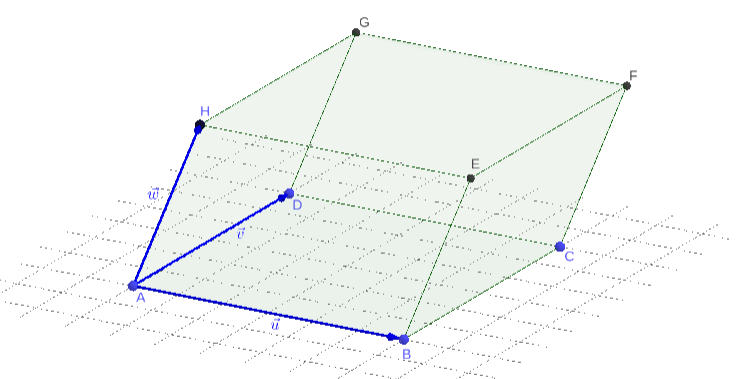
\includegraphics[width=0.8\textwidth]{cap_prodmisto/dados/fig_pm_ig/fig_pm_ig}
  \caption{Interpretação geométrica do produto misto.}
  \label{fig:pm_ig}
\end{figure}

A base do paralelepípedo é o paralelogramo $ABCD$ de área $|\vec{u}\land\vec{v}|$. Assim sendo, o \emph{volume do paralelepípedo} é
\begin{equation}\label{eq:pm_aux1}
  V = |\vec{u}\land\vec{v}|\cdot h,
\end{equation}
onde $h$ é a altura do prisma. Por sua vez,
\begin{align}
  h &= \left|\proj_{\vec{u}\land\vec{v}}\vec{w}\right| \\
    &= \left|\frac{\vec{w}\cdot(\vec{u}\land\vec{v})}{|\vec{u}\land\vec{v}|^2}\vec{u}\land\vec{v}\right|\\
    &= \frac{\left|\vec{w}\cdot(\vec{u}\land\vec{v})\right|}{|\vec{u}\land\vec{v}|^2}|\vec{u}\land\vec{v}|\\
    &= \frac{\left|\vec{w}\cdot(\vec{u}\land\vec{v})\right|}{|\vec{u}\land\vec{v}|} 
\end{align}
Logo, retornando a \eqref{eq:pm_aux1}, obtemos
\begin{align}
  V &= |\vec{u}\land\vec{v}|\cdot h\\
    &= |\vec{u}\land\vec{v}|\cdot\frac{\left|\vec{w}\cdot(\vec{u}\land\vec{v})\right|}{|\vec{u}\land\vec{v}|} \\
    &= \left|\vec{w}\cdot(\vec{u}\land\vec{v})\right|\\
    &= \left|\vec{u}\land\vec{v}\cdot\vec{w}\right|.
\end{align}
Ou seja, o \emph{volume do paralelepípedo} formado pelos vetores $\vec{u}$, $\vec{v}$ e $\vec{w}$ é igual a norma do produto misto destes vetores, i.e.
\begin{equation}\label{eq:pm_vp}
  {\color{blue}V = |[\vec{u},\vec{v},\vec{w}]|}.
\end{equation}

\begin{ex}
  Vamos calcular o volume do paralelepípedo determinado pelos vetores $\vec{u}=(1,1,0)$, $\vec{v}=(-1,2,0)$ e $\vec{w}=(0,1,1)$. De \eqref{eq:pm_vp}, temos
  \begin{gather}
    V = |[\vec{u},\vec{v},\vec{w}]| \\
    = \left|
      \begin{vmatrix}
        1 & 1 & 0 \\
        -1 & 2 & 0 \\
        0 & 1 & 1
      \end{vmatrix}
    \right| \\
    = |3| = 3.
  \end{gather}
\end{ex}

\subsection{Propriedades}

Valem as seguintes propriedades:
\begin{enumerate}[a)]
\item {\color{blue}$[\vec{u},\vec{v},\vec{w}] = -[\vec{v},\vec{u},\vec{w}]$}

  {\it Demonstração}. De fato, quando permutamos duas linhas em uma matriz, seu determinante troca de sinal.
  
\item {\color{blue}$[\vec{u},\vec{v},\vec{w}] = -[\vec{u},\vec{w},\vec{v}]$}

  {\it Demonstração.} Mesmo argumento da letra a).
  
\item {\color{blue}$[\vec{u},\vec{v},\vec{w}] = [\vec{w},\vec{u},\vec{v}] = [\vec{v},\vec{w},\vec{u}]$}

  {\it Demonstração.} De fato, cada caso acima corresponde a duas consecutivas permutações de linha na matriz associada ao produto misto.
  
\item {\color{blue}$[\vec{u},\vec{v},\vec{w}] = \vec{u}\land\vec{v}\cdot\vec{w} = \vec{u}\cdot\vec{v}\land\vec{w}$}

  {\it Demonstração.} Isto segue de c), i.e.
  \begin{align}
    [\vec{u},\vec{v},\vec{w}] &= [\vec{v},\vec{w},\vec{u}] \\
    \vec{u}\land\vec{v}\cdot\vec{w} &= \vec{v}\land\vec{w}\cdot\vec{u}\\
                              &= \vec{u}\cdot\vec{v}\land\vec{w}.
  \end{align}
  
\item {\color{blue}$[\alpha\vec{u},\vec{v},\vec{w}] = [\vec{u},\alpha\vec{v},\vec{w}]=[\vec{u},\vec{v},\alpha\vec{w}] = \alpha[\vec{u},\vec{v},\vec{w}]$}

  {\it Determinação.} De fato, ao multiplicarmos uma linha de uma matriz por um escalar $\alpha$, seu determinante fica multiplicado por $\alpha$.
  
\item {\color{blue}$[\vec{u}+\vec{z},\vec{v},\vec{w}] = [\vec{u},\vec{v},\vec{w}]+[\vec{z},\vec{v},\vec{w}]$}

  {\it Determinante.} Também segue da propriedade análoga do determinante de matrizes.
\end{enumerate}

\begin{ex}
  Sabendo que $[\vec{u},2\vec{w},\vec{v}] = 2$, vamos calcular $[\vec{u},\vec{v},\vec{w}]$. Do item e) acima, temos
  \begin{align}
    2 &= [\vec{u},2\vec{w},\vec{v}] \\
      &= 2[\vec{u},\vec{w},\vec{v}],
  \end{align}
  donde
  \begin{equation}
    [\vec{u},\vec{w},\vec{v}] = 1.
  \end{equation}
  Agora, do item b), temos
  \begin{equation}
    [\vec{u},\vec{w},\vec{v}] = -[\vec{u},\vec{v},\vec{w}].
  \end{equation}
  Ou seja, concluímos que $[\vec{u},\vec{v},\vec{w}] =  -1$.
\end{ex}

Também, temos as seguinte propriedades envolvendo o produto misto:
\begin{enumerate}[a)]
\item Se ${\color{blue}[\vec{u},\vec{v},\vec{w}] = 0}$, então ${\color{blue}(\vec{u},\vec{v},\vec{w})}$ \emph{não é base}.

  {\it Demonstração}. Seja $[\vec{u},\vec{v},\vec{w}]=0$, i.e. $\vec{u}\land\vec{v}\cdot\vec{w}=0$. No caso de um dos vetores serem nulos, então $(\vec{u},\vec{v},\vec{w})$ não é base. Suponhamos, então, que $\vec{u}$, $\vec{v}$ e $\vec{w}$ são vetores não nulos. Isso implica que $\vec{u}\land\vec{v}=0$ ou $(\vec{u}\land\vec{v})\perp\vec{w}$. No primeiro caso, $\vec{u}$ e $\vec{v}$ são l.d. e, portanto, $(\vec{u},\vec{v},\vec{w})$  não é base. No segundo caso, $(\vec{u}\land\vec{v})\perp\vec{w}$, temos que $\vec{w}$ é coplanar aos vetores $\vec{u}$ e $\vec{v}$, logo $(\vec{u},\vec{v},\vec{w})$ não é base.
  
\item Se ${\color{blue}[\vec{u},\vec{v},\vec{w}] > 0}$, então ${\color{blue}(\vec{u},\vec{v},\vec{w})}$ é uma \emph{base positiva}.

  {\it Demonstração.} Se $[\vec{u},\vec{v},\vec{w}] > 0$, implica que o ângulo entre $\vec{u}\land\vec{v}$ e $\vec{w}$ é agudo, o que garante que $(\vec{u},\vec{v},\vec{w})$ seja uma base positiva.
  
\item Se ${\color{blue}[\vec{u},\vec{v},\vec{w}] < 0}$, então ${\color{blue}(\vec{u},\vec{v},\vec{w})}$ é uma \emph{base negativa}.

  {\it Demonstração.} Se $[\vec{u},\vec{v},\vec{w}] < 0$, implica que o ângulo entre $\vec{u}\land\vec{v}$ e $\vec{w}$ é obtuso, o que garante que $(\vec{u},\vec{v},\vec{w})$ seja uma base negativa.
\end{enumerate}

\subsection*{Exercícios resolvidos}

\begin{exeresol}
  Calcule a área do paralelogramo determinado pelos vetores $\vec{v}=(1,0,-2)$, $\vec{w}=(1,-2,1)$ e $\vec{u}=(0,2,1)$.
\end{exeresol}
\begin{resol}
  Da Subseção \ref{subsec:pm_ig}, temos que o volume do paralelogramo é
  \begin{equation}
    V = |[\vec{u},\vec{v},\vec{w}]|,
  \end{equation}
  não importando a ordem dos vetores\footnote{A ordem dos vetores não altera o módulo do valor do produto misto.}. Assim sendo, temos
  \begin{gather}
    V = |[\vec{u},\vec{v},\vec{w}]| \\
    = \left|
      \begin{vmatrix}
        0 & 2 & 1 \\
        1 & 0 & -2 \\
        1 & -2 & 1 
      \end{vmatrix}
    \right| \\
    = |-8| = 8.
  \end{gather}
\end{resol}

\begin{exeresol}
  Sejam $\vec{u}$, $\vec{v}$ e $\vec{w}$ vetores dados. Verifique a seguinte afirmação:
  \begin{equation}
    [\vec{u},\vec{v}+\alpha\vec{u}+\beta\vec{w},\vec{w}]=[\vec{u},\vec{v},\vec{w}],
  \end{equation}
  onde $\alpha$ e $\beta$ são quaisquer escalares.
\end{exeresol}
\begin{resol}
  Das propriedades do produto misto\footnote{$[\vec{u},\vec{v}+\vec{z},\vec{w}]=[\vec{u},\vec{v},\vec{w}]+[\vec{u},\vec{z},\vec{w}]$.}, temos
  \begin{gather}
    [\vec{u},\vec{v}+\alpha\vec{u}+\beta\vec{w},\vec{w}] \\
    = [\vec{u},\vec{v},\vec{w}] + [\vec{u},\alpha\vec{u}+\beta\vec{w},\vec{w}].
  \end{gather}
  Agora, observamos que $\alpha\vec{u}+\beta\vec{w}$ é combinação linear de $\vec{u}$ e $\vec{v}$, logo $(\vec{u}, \alpha\vec{u}+\beta\vec{w}, \vec{w})$ é l.d. e, portanto,
  \begin{equation}
    [\vec{u},\alpha\vec{u}+\beta\vec{w},\vec{w}] = 0.
  \end{equation}
  Concluímos que
  \begin{equation}
  [\vec{u},\vec{v}+\alpha\vec{u}+\beta\vec{w},\vec{w}]=[\vec{u},\vec{v},\vec{w}].  
  \end{equation}
\end{resol}


\subsection*{Exercícios}

\begin{exer}
  Calcule $[\vec{u},\vec{v},\vec{w}]$ sendo $\vec{u}=(-1,0,1)$, $\vec{v}=(1,3,0)$ e $\vec{w}=(1,-2,-1)$.
\end{exer}
\begin{resp}
  -2
\end{resp}

\begin{exer}
  Sejam $\vec{a}=(0,0,2)$, $\vec{d}=(-1,1,1)$ e $\vec{e}=(1,1,1)$. Calcule $[\vec{d},\vec{a},\vec{e}]$.
\end{exer}
\begin{resp}
  $4$
\end{resp}

\begin{exer}
  Sendo $[\vec{u},\vec{v},\vec{w}]=2$, calcule $[2\vec{u},-3\vec{v},\vec{w}]$.
\end{exer}
\begin{resp}
  $-12$
\end{resp}

\begin{exer}
  Sendo $[\vec{u},\vec{v},\vec{w}]=2$, calcule $[2\vec{u}-5\vec{w},-3\vec{v},\vec{w}]$.
\end{exer}
\begin{resp}
  $-12$
\end{resp}

\begin{exer}
  Sejam $\vec{u}=(0,x,2)$, $\vec{v}=(-1,1,1)$ e $\vec{w}=(1,1,1)$. Calcule $x$ de forma que $[\vec{u},\vec{v},\vec{w}]=2$.
\end{exer}
\begin{resp}
  $3$
\end{resp}

%%Este trabalho está licenciado sob a Licença Atribuição-CompartilhaIgual 4.0 Internacional Creative Commons. Para visualizar uma cópia desta licença, visite http://creativecommons.org/licenses/by-sa/4.0/deed.pt_BR ou mande uma carta para Creative Commons, PO Box 1866, Mountain View, CA 94042, USA.

\chapter{Estudo de retas e planos}\label{cap_erp}
\thispagestyle{fancy}

\section{Sistema de coordenadas no espaço}\label{cap_erp_sec_siscoord}

Um sistema de coordenadas no espaço é constituído de um ponto $O$ e uma base de vetores $B = (\vec{e}_1, \vec{e}_2, \vec{e}_3)$ no espaço. Dado um tal sistema, temos que cada ponto $P$ determina de forma única um vetor $\overrightarrow{OP} = (x,y,z)$ e vice-versa. Assim sendo, definimos que o ponto $P$ tem coordenadas $(x,y,z)$.

O ponto $O$ é chamado de \emph{origem} (do sistema de coordenados) e tem coordenadas $(0,0,0)$. Dado um ponto $P=(x,y,z)$, chama-se $x$ de sua \emph{abscissa}, $y$ de sua \emph{ordenada} e $z$ de sua \emph{cota}. As retas que passam por $O$ e têm, respectivamente, as mesmas direções de $\vec{e}_1$, $\vec{e}_2$ e $\vec{e}_3$ são chamadas de \emph{eixo das abscissas}, \emph{eixo das ordenadas} e \emph{eixo das cotas}. Os planos que contém $O$ e representantes de dois vetores da base $B$ são chamados de \emph{planos coordenados}.

\begin{figure}[H]
  \centering
  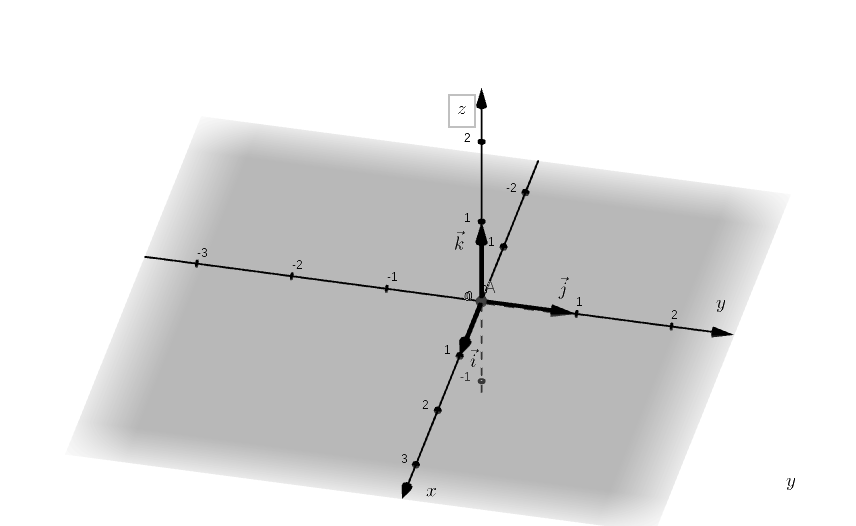
\includegraphics[width=0.7\textwidth]{./cap_erp/dados/fig_sis_coord_orto/fig_sis_coord_orto}
  \caption{Sistema de coordenadas ortonormal.}
  \label{fig:sis_coord_orto}
\end{figure}

Salvo explicitado ao contrário, trabalharemos com \emph{sistemas de coordenadas ortogonais}, i.e. sistema cuja base $B = (\vec{i},\vec{j},\vec{k})$ seja ortonormal. Mais ainda, estaremos assumindo que a base é positiva. Veja a Figura \ref{fig:sis_coord_orto}.

\begin{obs}\normalfont{(Relação entre pontos e vetores)}
  Seja dado um vetor $\overrightarrow{AB}$. Sabendo as coordenadas dos pontos $A = (x_A,y_A,z_A)$ e $B = (x_B,y_B,z_B)$, temos que as coordenadas do vetor $\overrightarrow{AB}$ são:
  \begin{align}
    \overrightarrow{AB} &= \overrightarrow{AO} + \overrightarrow{OB}\\
                        &= -\overrightarrow{OA} + \overrightarrow{OB}\\
                        &= -(x_A,y_A,z_A)+(x_B,y_B,z_B)\\
                        &= (x_B-x_A,y_B-y_A,z_B-z_A).
  \end{align}
\end{obs}

\begin{ex}
  Dados os pontos $A = (-1,1,2)$ e $B = (3,-1,0)$, temos que o vetor $\overrightarrow{AB}$ tem coordenadas:
  \begin{equation}
    \overrightarrow{AB} = (3-(-1),-1-1,0-2) = (4,-2,-2).
  \end{equation}
\end{ex}

\begin{obs}\normalfont{(Ponto médio de um segmento)}
  Dados os pontos $A = (x_A,y_A,z_A)$ e $B = (x_B,y_B,z_B)$, podemos calcular as coordenadas do ponto médio $M = (x_M,y_M,z_M)$ do segmento $AB$, do fato de que $\overrightarrow{AM} = \overrightarrow{MB}$. Portanto
  \begin{equation}
    (x_M-x_A,y_M-y_A,z_M-z_A)=(x_B-x_M,y_B-y_M,z_B-z_M),
  \end{equation}
  donde
  \begin{align}
    2x_M &= x_A+x_B\\
    2y_M &= y_A+y_B\\
    2z_M &= z_A+z_B.
  \end{align}
  Logo, temos $\displaystyle M = \left(\frac{x_A+x_B}{2},\frac{y_A+y_B}{2},\frac{z_A+z_B}{2}\right)$.
\end{obs}

\begin{ex}
  Dados os pontos $A = (-1,1,2)$ e $B = (3,-1,0)$, temos que o ponto médio do segmento $AB$ tem coordenadas:
  \begin{equation}
    M = \left(\frac{-1+3}{2},\frac{1+(-1)}{2},\frac{2+0}{2}\right) = (1,0,1).
  \end{equation}
\end{ex}

\subsection*{Exercícios resolvidos}

\begin{exeresol}
  Sejam $A = (-1,2,1)$, $B = (1,-2,0)$ e $C = (x,2,2)$ vértices consecutivos de um triângulo isósceles, cujos lados $AC$ e $BC$ são congruentes. Determine o valor de $x$.
\end{exeresol}
\begin{resol}
  Sendo os lados $AC$ e $BC$ congruentes, temos $|\overrightarrow{AC}| = |\overrightarrow{BC}|$. As coordenadas de $\overrightarrow{AC}$ são
  \begin{equation}
    \overrightarrow{AC} = (x-(-1),2-2,2-1) = (x+1,0,1)
  \end{equation}
  e as coordenadas de $\overrightarrow{BC}$ são
  \begin{equation}
    \overrightarrow{BC} = (x-1,2-(-2),2-0) = (x-1,4,2).
  \end{equation}
  Então, temos
  \begin{align}
    |\overrightarrow{AC}| = |\overrightarrow{BC}| &\Rightarrow \sqrt{(x+1)^2+0^2+1^2} = \sqrt{(x-1)^2+4^2+2^2}\\
                                                  &\Rightarrow (x+1)^2+0^2+1^2 = (x-1)^2+4^2+2^2\\
                                                  &\Rightarrow x^2+2x+1+1 = x^2-2x+1+16+4\\
                                                  &\Rightarrow 4x = 19\\
                                                  &\Rightarrow x = \frac{19}{4}.
  \end{align}
\end{resol}

\begin{exeresol}
  Sejam $A = (-1,2,1)$, $B = (1,-2,0)$  e $M$ o ponto médio do intervalo $AB$. Determine as coordenadas do ponto $P$ de forma que $2AP = AM$.
\end{exeresol}
\begin{resol}
  As coordenadas do ponto médio são
  \begin{equation}
    M = \left(\frac{-1+1}{2},\frac{2+(-2)}{2},\frac{1+0}{2}\right) = \left(0,0,\frac{1}{2}\right).
  \end{equation}
  Agora, denotando $P = (x_P,y_P,z_P)$, temos
  \begin{align}
    2AP = AM &\Rightarrow 2(x_P-(-1),y_P-2,z_P-1) = \left(0-(-1),0-2,\frac{1}{2}-1\right)\\
             &\Rightarrow (2x_p+2,2y_P-4,2z_P-2) = \left(1,-2,-\frac{1}{2}\right).
  \end{align}
  Portanto
  \begin{align}
    & 2x_P+2 = 1 \Rightarrow x_P = -\frac{1}{2}\\
    & 2y_P-4 = -2 \Rightarrow y_P = 1\\
    & 2z_P-2 = -\frac{1}{2} \Rightarrow z_P = \frac{3}{4}.
  \end{align}
  Logo, $P = (-1/2,1,3/4)$.
\end{resol}

\subsection*{Exercícios}

\emconstrucao

\section{Equações da reta}\label{cap_ert_sec_eqsreta}

\emconstrucao

%%Este trabalho está licenciado sob a Licença Atribuição-CompartilhaIgual 4.0 Internacional Creative Commons. Para visualizar uma cópia desta licença, visite http://creativecommons.org/licenses/by-sa/4.0/deed.pt_BR ou mande uma carta para Creative Commons, PO Box 1866, Mountain View, CA 94042, USA.

\chapter{Cônicas}\label{cap_conicas}
\thispagestyle{fancy}

Neste capítulo, fazemos um estudo introdutório sobre cônicas no plano cartesiano. Mais precisamente, vamos estudar as equações de elipses, hipérboles e parábolas.

\section{Elipse}\label{cap_conicas_sec_elipse}

Sejam $F_1$, $F_2$ pontos sobre um plano $\pi$, $c = \frac{1}{2}|F_1F_2|$ e $a > c$. Chama-se \emph{elipse} de \emph{focos} $F_1$ e $F_2$ ao conjunto de pontos $P$ tais que
\begin{equation}
  {\color{blue}|PF_1| + |PF_2| = 2a}.
\end{equation}
Veja a Figura \ref{fig:elipse}.

\begin{figure}[H]
  \centering
  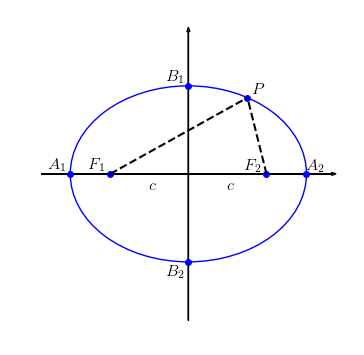
\includegraphics[width=0.7\textwidth]{./cap_conicas/dados/fig_elipse/fig_elipse}
  \caption{Ilustração de uma elipse de focos $F_1$ e $F_2$.}
  \label{fig:elipse}
\end{figure}

Dada uma tal elipse, identificamos $2c=|F_1F_2|$ como a \emph{distância focal}. Os pontos $A_1$ e $A_2$ de interseção da elipse com a reta que passa pelos focos são chamados de \emph{vértices} da elipse. O segmento $A_1A_2$ é chamado de \emph{eixo maior} da elipse. Observamos que
\begin{equation}
  |A_1A_2| = 2a.
\end{equation}
O ponto médio do segmento $F_1F_2$ é chamado de \emph{centro} da elipse. Sejam $B_1$ e $B_2$ os pontos de interseção da elipse com a reta que passa pelo centro da elipse e é perpendicular ao segmento $A_1A_2$. Assim sendo, o segmento $B_1B_2$ é chamado de \emph{eixo menor} da elipse. Vamos denotar
\begin{equation}
  2b = |B_1B_2|.
\end{equation}

Chamamos de \emph{excentricidade} da elipse o número
\begin{equation}
  e = \frac{c}{a}.
\end{equation}
Notemos que $0 \leq e < 1$. Para $e=0$, temos $c=0$ e, portanto $F_1=F_2$. Neste caso, a elipse é a circunferência de centro em $F_1$ (ou $F_2$) e diâmetro $2a$. No que $e$ tende a $1$, a elipse tende ao segmento $A_1A_2$.

Por fim, notamos que o triângulo $B_1OF_2$ é retângulo, $|OF_2|=c$, $|F_2B_1|=a$ e $|OB_1|=b$. Do teorema de Pitágoras segue
\begin{equation}\label{eq:elipse_obs}
  b^2 + c^2 = a^2.
\end{equation}

\subsection{Equação reduzida da elipse}

Consideremos o sistema de coordenadas cartesianas. Sejam $F_1=(-c,0)$ e $F_2=(c,0)$, $c\geq 0$, os focos de uma dada elipse (veja a Figura \ref{fig:elipse}).  Se $P=(x,y)$ é um ponto da elipse, então
\begin{equation}
  |PF_1| + |PF_2| = 2a.
\end{equation}
Como
\begin{align}
  |PF_1| &= \sqrt{(x+c)^2 + y^2}, \\
  |PF_2| &= \sqrt{(x-c)^2 + y^2},
\end{align}
temos
\begin{equation}
  \sqrt{(x+c)^2 + y^2} + \sqrt{(x-c)^2 + y^2} = 2a,
\end{equation}
ou, equivalentemente,
\begin{equation}
  \sqrt{(x+c)^2 + y^2} = 2a - \sqrt{(x-c)^2 + y^2}.
\end{equation}
Elevando ao quadrado, obtemos
\begin{equation}
  (x+c)^2 + y^2 = 4a^2 - 4a\sqrt{(x-c)^2+y^2} + (x-c)^2+y^2.
\end{equation}
Por cancelamento e rearranjo dos termos, obtemos
\begin{equation}
  a\sqrt{(x-c)^2+y^2}=a^2-cx.
\end{equation}
Elevando novamente ao quadrado, temos
\begin{equation}
  a^2(x-c)^2+a^2y^2=a^4-2a^2cx+c^2x^2,
\end{equation}
donde
\begin{equation}
  a^2x^2 -2a^2cx + a^2c^2 + a^2y^2= a^4 -2a^2cx + c^2x^2.
\end{equation}
Por cancelamento e rearranjo dos termos, obtemos
\begin{equation}
  x^2(a^2 - c^2) + a^2y^2 = a^2(a^2 - c^2).
\end{equation}
Como $a>c$, dividimos por $a^2-c^2$  e depois por $a^2$ para obtemos
\begin{equation}
  \frac{x^2}{a^2} + \frac{y^2}{a^2-c^2} = 1.
\end{equation}
Por fim, da equação \eqref{eq:elipse_obs}, temos $a^2-c^2 = b^2$, o que nos leva  a \emph{equação reduzida da elipse}
\begin{equation}
  {\color{blue}\frac{x^2}{a^2} + \frac{y^2}{b^2} = 1}.
\end{equation}

\begin{ex}
  A Figura \ref{fig:elipse_ex} é um esboço do gráfico da elipse de equação reduzida
  \begin{equation}
    \frac{x^2}{25} + \frac{y^2}{16} = 1.
  \end{equation}

  \begin{figure}[H]
    \centering
    \includegraphics[width=0.5\textwidth]{cap_conicas/dados/fig_ex_elipse/fig}
    \caption{Esboço do gráfico da elipse $\displaystyle\frac{x^2}{25}-\frac{y^2}{16}=1$.}
    \label{fig:elipse_ex}
  \end{figure}
\end{ex}

\subsection*{Exercícios resolvidos}

\begin{exeresol}
  Determine a equação reduzida da elipse de focos $F_1=(-3,0)$, $F_2=(3,0)$ e vértices $A_1=(-5,0)$ e $A_2=(5,0)$.
\end{exeresol}
\begin{resol}
  A equação reduzida tem a forma
  \begin{equation}
    \frac{x^2}{a^2} + \frac{y^2}{b^2} = 1,
  \end{equation}
  onde
  \begin{equation}
    b^2 + c^2 = a^2.
  \end{equation}
  Dos focos temos $c=3$ e dos vértices temos $a=5$. Logo,
  \begin{align}
    b^2 &=  a^2 - c^2 \\
        &= 5^2 - 3^2 \\
        &= 25 - 9 \\
        &= 16.
  \end{align}
  Concluímos que a elipse em questão tem equação
  \begin{equation}
    \frac{x^2}{25} - \frac{y^2}{16} = 1.
  \end{equation}
\end{resol}

\begin{exeresol}
  Determine os focos da elipse de equação
  \begin{equation}
    \frac{x^2}{16} + \frac{y^2}{25} = 1.
  \end{equation}
\end{exeresol}
\begin{resol}
  Começamos lembrando que os focos de uma elipse estão localizados sobre seu eixo maior. No caso deste exercício, temos $a=4$ e $b=5$, logo o eixo maior é $B_1B_2$, na mesma direção do eixo das ordenadas $Oy$. Do triângulo retângulo $OA_2F_1$ temos
  \begin{equation}
    b^2 = a^2 + c^2,
  \end{equation}
  veja a Figura \ref{fig:elipse_exeresol1}.

  \begin{figure}[H]
    \centering
    \includegraphics[width=0.5\textwidth]{cap_conicas/dados/fig_elipse_exeresol1/fig}
    \caption{Esboço do gráfico de uma elipse com eixo maior sobre o eixo das ordenadas $Oy$.}
    \label{fig:elipse_exeresol1}
  \end{figure}

  Daí, temos
  \begin{align}
    c^2 &= b^2 - a^2 \\
        &= 25 - 16 \\
        &= 9 \\
    c &= 3.
  \end{align}
  Concluímos que os focos são $F_1=(0,-3)$ e $F_2=(0,3)$.
\end{resol}

\subsection*{Exercícios}

\begin{exer}
  Faça um esboço da elipse de equação reduzida
  \begin{equation}
    \frac{x^2}{9} + \frac{y^2}{4} = 1.
  \end{equation}
\end{exer}
\begin{resp}
  \includegraphics[width=0.5\textwidth]{cap_conicas/dados/fig_elipse_exer_ox/fig}
\end{resp}

\begin{exer}
  Faça um esboço da elipse de equação reduzida
  \begin{equation}
    \frac{x^2}{4} + \frac{y^2}{9} = 1.
  \end{equation}
\end{exer}
\begin{resp}
  \includegraphics[width=0.4\textwidth]{cap_conicas/dados/fig_elipse_exer_oy/fig}
\end{resp}

\begin{exer}
  Determine os vértices (sobre o eixo maior) das seguintes elipses:
  \begin{enumerate}[a)]
  \item $\displaystyle \frac{x^2}{9} + \frac{y^2}{4} = 1$
  \item $\displaystyle x^2 + \frac{y^2}{16} = 1$
  \end{enumerate}
\end{exer}
\begin{resp}
  a)~$(-3, 0)$, $(3, 0)$; b)~$(0, -4)$, $(0, 4)$
\end{resp}

\begin{exer}
  Determine os focos das seguintes elipses:
  \begin{enumerate}[a)]
  \item $\displaystyle \frac{x^2}{9} + \frac{y^2}{4} = 1$
  \item $\displaystyle x^2 + \frac{y^2}{16} = 1$
  \end{enumerate}
\end{exer}
\begin{resp}
  a)~$(-\sqrt{5}, 0)$, $(\sqrt{5}, 0)$; b)~$(0, \sqrt{3})$, $(0, \sqrt{3})$
\end{resp}

\begin{exer}
  Forneça a equação reduzida da elipse de focos $F_1=(-1, 0)$, $F_2=(1, 0)$ e vértices $A_1=(-\sqrt{2}, 0)$, $A_2=(\sqrt{2}, 0)$.
\end{exer}
\begin{resp}
  $\displaystyle\frac{x^2}{2}+y^2=1$
\end{resp}

\begin{exer}
  Forneça a equação reduzida da elipse de focos $F_1=(0, -2)$, $F_2=(0, 2)$ e vértices $B_1=(0, -\sqrt{5})$, $B_2=(0, \sqrt{5})$.
\end{exer}
\begin{resp}
  $\displaystyle x^2+\frac{y^2}{5}=1$
\end{resp}

\section{Hipérbole}\label{cap_conicas_sec_hiperbole}

Sejam $F_1$ e $F_2$ pontos sobre um plano $\pi$. Sejam, também, $c$ tal que $|F_1F_2|=2c$ e $a<c$. O lugar geométrico dos pontos $P$ tais que
\begin{equation}
  {\color{blue}||PF_1|-|PF_2||=2a},
\end{equation}
chama-se \emph{hipérbole}. Veja Figura \ref{fig:hiperbole}.

\begin{figure}[H]
  \centering
  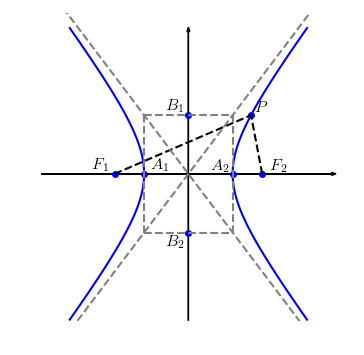
\includegraphics[width=0.7\textwidth]{./cap_conicas/dados/fig_hiperbole/fig_hiperbole}
  \caption{Ilustração de uma hipérbole de focos $F_1$ e $F_2$.}
  \label{fig:hiperbole}
\end{figure}

Os pontos $F_1$ e $F_2$ são chamados de \emph{focos} da hipérbole e $2c = |F_1F_2|$ é chamada de \emph{distância focal}. O ponto médio entre os pontos $F_1$ e $F_2$ é chamado de centro da hipérbole. São chamados \emph{vértices} da hipérbole os pontos $A_1$ e $A_2$, sendo que o segmento $A_1A_2$ é chamado de \emph{eixo real} (ou transverso) da hipérbole. O comprimento deste eixo é $|A_1A_2|=2a$.

Sejam $B_1$ e $B_2$ pontos $c$ distantes de $A_1$ e $A_2$ e pertencentes a reta que passa pelo centro da hipérbole e é perpendicular ao seu eixo real. O segmento $B_1B_2$ é chamado de \emph{eixo imaginário} (transverso ou conjugado). Denotando $2b=|B_1B_2|$, temos do triângulo retângulo $B_1OA_1$ que
\begin{equation}
  {\color{blue}c^2 = a^2 + b^2}.
\end{equation}

\subsection{Equação reduzida da hipérbole}

Assumimos um sistema de coordenadas cujo centro coincida com o centro de uma dada hipérbole e o eixo das abscissas seja coincidente com o eixo real da hipérbole. Desta forma, temos $F_1 = (-c,0)$ e $F_2 = (c,0)$. Então, $P=(x,y)$ é um ponto da hipérbole quando
\begin{equation}
  ||PF_1|-|PF_2|| = 2a.
\end{equation}
Daí, segue que
\begin{gather}
  |PF_1|-|PF_2| = \pm 2a \\
  \sqrt{(x+c)^2+y^2}-\sqrt{(x-c)^2+y^2} =\pm 2a\\
  \sqrt{(x+c)^2+y^2} = \pm 2a + \sqrt{(x-c)^2+y^2}
\end{gather}
Elevando ao quadrado ambos os lados desta última equação, obtemos
\begin{align}
  (x+c)^2+y^2 &= 4a^2 \pm 4a\sqrt{(x-c)^2+y^2} \\
              &+ (x-c)^2+y^2
\end{align}
ou, equivalentemente,
\begin{align}
  x^2+2cx+c^2+y^2 &= 4a^2\pm4a\sqrt{(x-c)^2+y^2}\\
                  &+x^2-2cx+c^2+y^2
\end{align}
Simplificando e rearranjando os termos, temos
\begin{equation}
  cx - a^2 = \pm a\sqrt{(x-c)^2+y^2}).
\end{equation}
Elevando novamente ao quadrado, obtemos
\begin{equation}
  c^2x^2 - 2a^2cx + a^4 = a^2x^2 - 2a^2cx + a^2c^2 + a^2y^2.
\end{equation}
Simplificando e rearranjando os termos, obtemos
\begin{equation}
  (c^2-a^2)x^2 - a^2y^2 = a^2(c^2-a^2).
\end{equation}
Lembrando que $c^2 = a^2 + b^2$, temos
\begin{equation}
  b^2x^2 - a^2y^2 = a^2b^2.
\end{equation}
Dividindo por $a^2b^2$, obtemos
\begin{equation}\label{eq:hiperbole_red}
  {\color{blue}\frac{x^2}{a^2} - \frac{y^2}{b^2} = 1},
\end{equation}
a qual é chamada de \emph{equação reduzida da hipérbole}.

\begin{ex}
  A Figura \ref{fig:ex_hiperbole} é um esboço do gráfico da hipérbole de equação reduzida
  \begin{equation}
    \frac{x^2}{16} - \frac{y^2}{9} = 1.
  \end{equation}

  \begin{figure}[H]
    \centering
    \includegraphics[width=0.7\textwidth]{cap_conicas/dados/fig_ex_hiperbole/fig}
    \caption{Esboço do gráfico da hipérbole de equação $\displaystyle\frac{x^2}{16}-\frac{y^2}{9}=1$.}
    \label{fig:ex_hiperbole}
  \end{figure}  
\end{ex}

\subsection*{Exercícios resolvidos}

\begin{exeresol}
  Obtenha a equação reduzida da hipérbole centrada na origem e de eixo real $|A_1A_2|=8$ e eixo imaginário $|B_1B_2|=4$.
\end{exeresol}
\begin{resol}
  A equação reduzida de uma hipérbole centrada na origem tem a forma
  \begin{equation}
    \frac{x^2}{a^2} - \frac{y^2}{b^2} = 1,
  \end{equation}
  onde $2a = |A_1A_2|$ e $2b=|B_1B_2|$. No caso deste exercício, temos
  \begin{equation}
    2a = 8 \Rightarrow a = 4
  \end{equation}
  e
  \begin{equation}
    2b = 4 \Rightarrow b = 2
  \end{equation}
  Logo, a equação buscada é
  \begin{equation}
    \frac{x^2}{4^2} - \frac{y^2}{2^2} = 1
  \end{equation}
  ou, equivalentemente,
  \begin{equation}
    \frac{x^2}{16} - \frac{y^2}{4} = 1.
  \end{equation}  
\end{resol}

\begin{exeresol}
  Faça o esboço da hipérbole de equação reduzida
  \begin{equation}
    \frac{y^2}{16} - \frac{x^2}{9} = 1.
  \end{equation}
\end{exeresol}
\begin{resol}
  Observe que nesta equação, o termo contendo $x$ tem sinal negativo e o termo contendo $y$ tem sinal positivo (compare com \eqref{eq:hiperbole_red}). Isto nos indica que o eixo real desta hipérbole está na direção das ordenadas $Oy$ e, consequentemente, o eixo imaginário na direção das abscissas $Ox$.

  Da equação, temos $a^2 = 9$ e $b^2=16$, donde $a=3$ e $b=4$. Neste caso, os vértices que definem o eixo real são $A_1=(0, -b)=(0, -4)$ e $A_2=(0, b)=(0, 4)$. Os focos $F_1=(0, -c)$ e $F_2=(0, c)$ são tais que
  \begin{align}
    c^2 &= a^2 + b^2 \\
        &= 9 + 16 \\a
        &= 25 \\
    c &= 5.
  \end{align}
  Com estas informações, traçamos o esboço dado na Figura \ref{fig:hiperbole_exeresol_oy}.

  \begin{figure}[H]
    \centering
    \includegraphics[width=0.5\textwidth]{cap_conicas/dados/fig_hiperbole_exeresol_oy/fig}
    \caption{Esboço do gráfico da hipérbole de equação $\displaystyle\frac{y^2}{16}-\frac{x^2}{9}=1$.}
    \label{fig:hiperbole_exeresol_oy}
  \end{figure}   
\end{resol}

\begin{exeresol}
  Mostre que uma hipérbole de equação reduzida
  \begin{equation}
    \frac{x^2}{a^2} - \frac{y^2}{b^2} = 1
  \end{equation}
  tem assíntotas
  \begin{equation}
    y = \pm \frac{b}{a}x.
  \end{equation}
\end{exeresol}
\begin{resol}
  De fato, ao isolarmos $y$ na equação reduzida, obtemos
  \begin{equation}
    y = \pm\sqrt{\frac{b^2}{a^2}x^2 - b^2}
  \end{equation}
  Logo, para $x\to \infty$, temos
  \begin{gather}
    y\to \pm\sqrt{\frac{b^2}{a^2}x^2} \\
    y\to \pm\sqrt{\frac{b^2}{a^2}}\sqrt{x^2}\\
    y\to \pm\frac{b}{a}x
  \end{gather}
  De forma análoga, quando $x\to -\infty$, temos
  \begin{gather}
    y\to \pm\sqrt{\frac{b^2}{a^2}x^2} \\
    y\to \pm\sqrt{\frac{b^2}{a^2}}\sqrt{x^2}\\
    y\to \mp\frac{b}{a}x
  \end{gather}
  Ambos os resultados mostram que $\displaystyle y=\pm\frac{b}{a}x$ são assíntotas da hipérbole.
\end{resol}

\subsection*{Exercícios}

\begin{exeresol}
  Faça o esboço da hipérbole de equação reduzida
  \begin{equation}
    \frac{x^2}{9} - \frac{y^2}{4} = 1
  \end{equation}
\end{exeresol}
\begin{resp}
  \includegraphics[width=0.5\textwidth]{cap_conicas/dados/fig_hiperbole_exer_ox/fig}
\end{resp}

\begin{exeresol}
  Faça o esboço da hipérbole de equação reduzida
  \begin{equation}
    \frac{y^2}{9} - \frac{x^2}{4} = 1
  \end{equation}
\end{exeresol}
\begin{resp}
  \includegraphics[width=0.5\textwidth]{cap_conicas/dados/fig_hiperbole_exer_oy/fig}
\end{resp}

\begin{exer}
  Determine os vértices do eixo real das seguintes hipérboles:
  \begin{enumerate}[a)]
  \item $\displaystyle \frac{x^2}{9} - \frac{y^2}{4} = 1$
  \item $\displaystyle y^2 - \frac{x^2}{16} = 1$
  \end{enumerate}
\end{exer}
\begin{resp}
  a)~$A_1=(-3,0)$, $A_2=(3,0)$; b)~$B_1=(0, -1)$, $B_2=(0, 1)$
\end{resp}

\begin{exer}
  Determine os focos das seguintes hipérboles:
  \begin{enumerate}[a)]
  \item $\displaystyle \frac{x^2}{9} - \frac{y^2}{4} = 1$
  \item $\displaystyle y^2 - \frac{x^2}{16} = 1$
  \end{enumerate}
\end{exer}
\begin{resp}
  a)~$F_1=(-\sqrt{13}, 0)$, $F_2=(\sqrt{13}, 0)$; b)~$F_1=(0, -\sqrt{17})$, $F_2=(0, \sqrt{17})$
\end{resp}

\begin{exer}
  Forneça a equação reduzida da hipérbole de focos $F_1=(-2, 0)$, $F_2=(2, 0)$ e de vértices do eixo real $A_1=(-1, 0)$ e $A_2=(1, 0)$.
\end{exer}
\begin{resp}
  $\displaystyle x^2 - \frac{y^2}{3} = 1$
\end{resp}

\begin{exer}
  Forneça a equação reduzida da hipérbole de distância focal $|F_1F_2|=2\sqrt{6}$ e de vértices do eixo imaginário $A_1=(-2, 0)$ e $A_2=(2, 0)$.
\end{exer}
\begin{resp}
  $\displaystyle \frac{y^2}{2} - \frac{x^2}{4} = 1$
\end{resp}

\section{Parábola}\label{cap_conicas_sec_parabola}

Em um plano, consideramos uma reta $d$ e um ponto $F$ não pertencente a $d$. Chamamos de \emph{parábola} o conjunto de pontos $P$ do plano que são equidistantes de $F$ e de $d$, i.e.
\begin{equation}
  {\color{blue}\dist(P, F) = \dist(P, d)}.
\end{equation}
Veja a Figura \ref{fig:parabola}.

\begin{figure}[H]
  \centering
  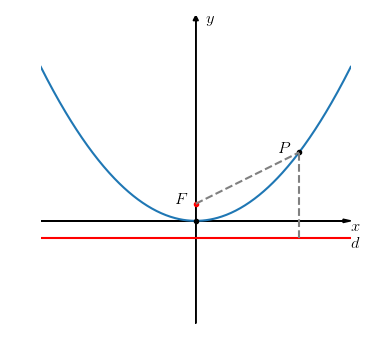
\includegraphics[width=0.7\textwidth]{./cap_conicas/dados/fig_parabola/fig_parabola}
  \caption{Ilustração de uma parábola.}
  \label{fig:parabola}
\end{figure}

O ponto $F$ é chamado de \emph{foco} da parábola. A reta $d$ é chamada de \emph{diretriz} da parábola. A reta perpendicular a $d$ e que passa pelo ponto $F$ é chamada de \emph{eixo} da parábola. O ponto $V$ de interseção entre a parábola e seu eixo é chamado de \emph{vértice} da parábola.

\subsection{Equação reduzida de uma parábola}

Tomamos o sistema cartesiano de coordenadas com origem no vértice da parábola e eixo das abscissas paralelo à diretriz. Seja $p$ tal que
\begin{equation}
  F = (0, p/2).
\end{equation}
Logo, a diretriz tem equação $y = -p/2$. Da definição de parábola, $P=(x,y)$ pertence a parábola quando
\begin{equation}
  \dist(P, F) = \dist(P, d).
\end{equation}
Segue que
\begin{equation}
  \sqrt{x^2+\left(y-\frac{p}{2}\right)^2} = y+\frac{p}{2}.
\end{equation}
Elevando ao quadrado e expandindo, obtemos
\begin{equation}
  x^2 + y^2-py+\frac{p^2}{4} = y^2 + py + \frac{p^2}{4}.
\end{equation}
Cancelando e rearranjando termos, obtemos
\begin{equation}
  {\color{blue}x^2 = 2py},
\end{equation}
a chamada \emph{equação reduzida da parábola}.

\begin{ex}
  A Figura \ref{fig:parabola_ex} é um esboço do gráfica da parábola de equação reduzida
  \begin{equation}
    x^2 = 4y.
  \end{equation}

  \begin{figure}[H]
    \centering
    \includegraphics[width=0.6\textwidth]{cap_conicas/dados/fig_parabola_ex/fig}
    \caption{Esboço do gráfico da parábola de equação $y^2 = 4x$.}
    \label{fig:parabola_ex}
  \end{figure}
\end{ex}

\begin{obs}
  Uma parábola com vértice na origem do sistema cartesiano e foco $F=(p/2, 0)$, tem equação reduzida
  \begin{equation}
    y^2 = 2px.
  \end{equation}
\end{obs}

\subsection*{Exercícios resolvidos}

\begin{exeresol}
  Determine a equação reduzida da parábola de diretriz $y=2$ e vértice na origem do sistema cartesiano. Por fim, faça o esboço de seu gráfico.
\end{exeresol}
\begin{resol}
  Uma parábola de equação reduzida
  \begin{equation}
    x^2 = 2py
  \end{equation}
  tem diretriz $\displaystyle y=-\frac{p}{2}$. Logo, sabendo que a diretriz é $y=2$, temos $p = -4$. Então, concluímos que a equação reduzida da parábola é
  \begin{equation}
    x^2 = -8y
  \end{equation}
  A Figura \ref{fig:parabola_exeresol_yp} é o esboço do gráfico desta parábola.

  \begin{figure}[H]
    \centering
    \includegraphics[width=0.6\textwidth]{cap_conicas/dados/fig_parabola_exeresol_yp/fig}
    \caption{Esboço do gráfico da parábola de equação $y^2 = -8x$.}
    \label{fig:parabola_exeresol_yp}
  \end{figure}  
\end{resol}

\begin{exeresol}
  Determine a equação reduzida da parábola de diretriz $x=2$ e vértice na origem do sistema cartesiano. Por fim, faça o esboço de seu gráfico.
\end{exeresol}
\begin{resol}
  Uma parábola de equação reduzida
  \begin{equation}
    y^2 = 2px
  \end{equation}
  tem diretriz $\displaystyle x=-\frac{p}{2}$. Logo, sabendo que a diretriz é $x=2$, temos $p = -4$. Então, concluímos que a equação reduzida da parábola é
  \begin{equation}
    y^2 = -8x
  \end{equation}
  A Figura \ref{fig:parabola_exeresol_xp} é o esboço do gráfico desta parábola.

  \begin{figure}[H]
    \centering
    \includegraphics[width=0.6\textwidth]{cap_conicas/dados/fig_parabola_exeresol_xp/fig}
    \caption{Esboço do gráfico da parábola de equação $y^2 = -8x$.}
    \label{fig:parabola_exeresol_xp}
  \end{figure}  
\end{resol}

\subsection*{Exercícios}

\begin{exer}
  Faça o esboço do gráfico da parábola de equação reduzida
  \begin{equation}
    x^2 = 2y.
  \end{equation}
  Identifique no esboço a reta diretriz, o foco e o vértice da parábola.
\end{exer}
\begin{resp}
  \includegraphics[width=0.5\textwidth]{cap_conicas/dados/fig_parabola_exer_x2_2y/fig}
\end{resp}

\begin{exer}
  Faça o esboço do gráfico da parábola de equação reduzida
  \begin{equation}
    x^2 = -2y.
  \end{equation}
  Identifique no esboço a reta diretriz, o foco e o vértice da parábola.
\end{exer}
\begin{resp}
  \includegraphics[width=0.5\textwidth]{cap_conicas/dados/fig_parabola_exer_x2-2y/fig}
\end{resp}

\begin{exer}
  Faça o esboço do gráfico da parábola de equação reduzida
  \begin{equation}
    y^2 = 2x.
  \end{equation}
  Identifique no esboço a reta diretriz, o foco e o vértice da parábola.
\end{exer}
\begin{resp}
  \includegraphics[width=0.5\textwidth]{cap_conicas/dados/fig_parabola_exer_y2_2x/fig}
\end{resp}

\begin{exer}
  Faça o esboço do gráfico da parábola de equação reduzida
  \begin{equation}
    y^2 = -2x.
  \end{equation}
  Identifique no esboço a reta diretriz, o foco e o vértice da parábola.
\end{exer}
\begin{resp}
  \includegraphics[width=0.5\textwidth]{cap_conicas/dados/fig_parabola_exer_y2-2x/fig}
\end{resp}

\begin{exer}
  Determine o foco de cada uma das seguintes parábolas:
  \begin{enumerate}[a)]
  \item $y = 2x^2$
  \item $y + 2x^2 = 0$
  \item $y^2 + 4x = 0$
  \item $\frac{1}{4}y^2 = x$
  \end{enumerate}
\end{exer}
\begin{resp}
  a)~$F=(0, \frac{1}{8})$; b)~$F=(0, -\frac{1}{8})$; c)~$F=(-1, 0)$; d)~$F=(1, 0)$
\end{resp}


%resposta dos exercícios
\ifisbook
%Este trabalho está licenciado sob a Licença Atribuição-CompartilhaIgual 4.0 Internacional Creative Commons. Para visualizar uma cópia desta licença, visite http://creativecommons.org/licenses/by-sa/4.0/ ou mande uma carta para Creative Commons, PO Box 1866, Mountain View, CA 94042, USA.

\chapter*{Resposta dos Exercícios}\label{cap_respostas}
\addcontentsline{toc}{chapter}{Respostas dos Exercícios}

\shipoutAnswer
\fi

%references
\nocite{*}
\bibliographystyle{plain}
\bibliography{main}
\addcontentsline{toc}{chapter}{Referências Bibliográficas}

\ifisbook
\clearpage
\addcontentsline{toc}{chapter}{Índice Remissivo}
\printindex
\fi

\end{document}
